\chapter{High Voltage}
\label{ch:sp-hv}
%%%%%%%%%%%%%%%%%%%%%%%%%%%%%%%%%%%%%%%%%%%%%%%%%%%%%%%%%%%%%%%%%%%%
\section{High Voltage System Overview}
\label{sec:fdsp-hv-ov}

%%%%%%%%%%%%%%%%%%%%%%%%%%%%
\subsection{Introduction and Scope}
\label{sec:fdsp-hv-intro}

A \dword{lartpc} requires an equipotential cathode plane at \dword{hv} and a precisely regulated interior electric field (\efield{}) to drive 
electrons from particle interactions to sensor planes.  To achieve this, the DUNE \dword{sp} \dword{tpc} consists of 
\begin{itemize}
\item vertical cathode planes, called \dword{cpa} arrays, held at \dword{hv};
\item vertical anode planes, called \dword{apa} arrays, described in Chapter~\ref{ch:fdsp-apa}; and
\item formed sets of conductors at graded voltages surrounding the
 the drift volumes to ensure uniformity of the \efield; the conductors are collectively called the \dword{fc}.
\end{itemize}

The \single \dword{tpc} configuration is shown in Figure~\ref{fig:dune_sp_fd}.
The  drift fields transport the ionization electrons 
towards the \dwords{apa} at the sides and center.

\begin{dunefigure}[One unit of the \dword{spmod}]
{fig:dune_sp_fd}
{A schematic of a \dword{spmod} showing the three \dword{apa} arrays (at the far left and right and in the center, all of which span the entire \sptpclen \dword{detmodule} length) and the two \dword{cpa} arrays, occupying the intermediate second and fourth positions. The top and bottom \dword{fc} modules are shown in blue; the \dwords{ewfc} are not shown. 
On the right, the front top and bottom \dword{fc} modules are shown (in blue) folded up against the \dword{cpa} panels to which they connect, as they are positioned for shipping and insertion into the cryostat.  The \dwords{cpa}, \dwords{apa}, and \dwords{fc} together define the four drift volumes of the \dword{spmod}. The sizes and quantities of the \dword{fc} and \dword{cpa}-array components are listed in Tables~\ref{tab:cpaparts} and~\ref{tab:fcparts} and represented in this image.}
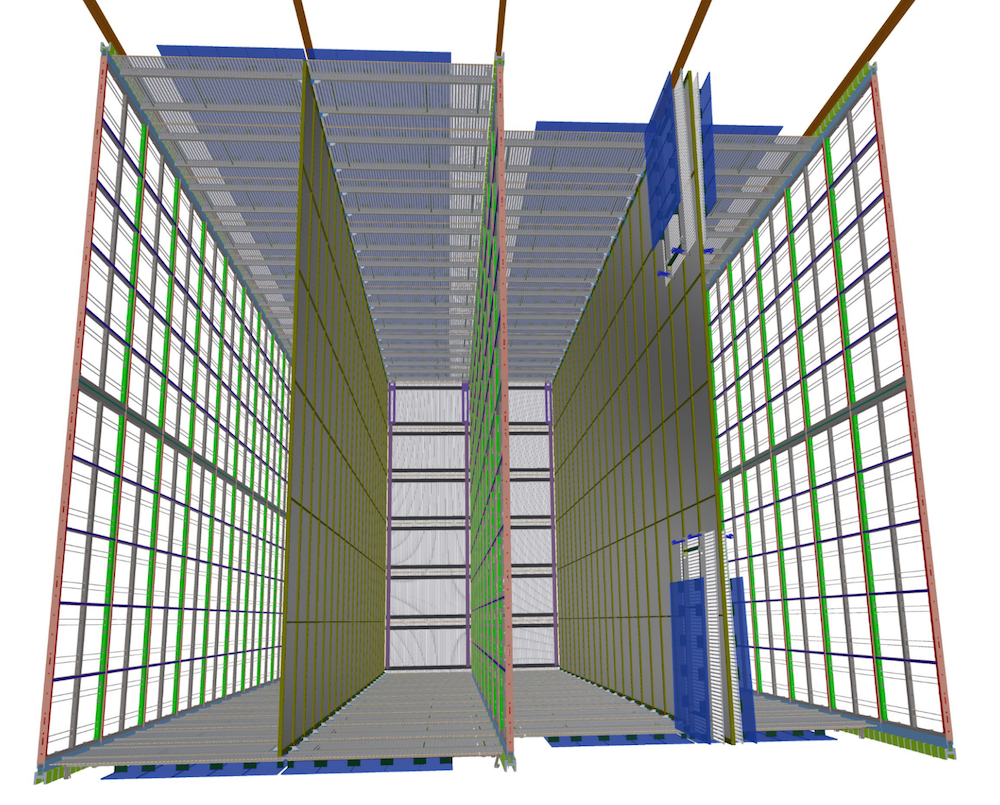
\includegraphics[width=0.95\textwidth]{dune_sp_fd}
\end{dunefigure}

%%%%%%%%%%%%%%%%%%%%%%%%%%%%
%\subsection{High Voltage System Scope}
%\label{sec:fdsp-hv-scope}

The scope of the \single \dword{hv} system, provided by the DUNE \dword{hv} consortium, includes the selection and procurement of materials for, and the fabrication, testing, delivery and installation of systems to generate, distribute, and regulate the voltages that
create a stable and precise \efield{} within a \dword{spmod}. 

The \dword{hv} system consists of components both exterior and interior to the cryostat. The voltage generated at the \dword{hv} power supplies passes through the cables, filters, and the \dword{hv} \fdth into the cryostat. From the point of delivery into the cryostat, components that form part of the \dword{tpc} structure further distribute the voltage. The internal \dword{hv} components in fact form a large fraction of the total internal structures of the \dword{tpc} itself, and  
 %largely 
 effectively bound the  fiducial volume of the %experiment 
 \dword{detmodule}. The \dword{hv} system plays a key role in determining the event rate for all DUNE physics processes.

The \dword{hv} system consists of
\begin{itemize}
\item \dword{hv} power supplies, cables, filters, and feedthroughs;
\item \dword{cpa} array;
\item \dword{topfc}, \dword{botfc}, and \dwords{gp}; and
\item \dword{ewfc}.
\end{itemize}


\fixme{for Brett: when I used Dword for topfc I got all caps; not true for ewfc. Anne}
The system operates at the full range of voltages, %all voltages, from the highest 
%maximum 
$-$\sptargetdriftvoltpos to ground, inside the \dword{tpc} volume. 

The \single and \dual modules will implement similar designs for some
 of the \dword{hv} system components, %including the \dwords{fc} profiles and supporting FRP beams, and the voltage divider boards. More details can be found in   
 in particular, aspects of the \dwords{fc} and its supporting beams. The single phase versions are described in this chapter. 
 %\fixme{for Anne  let's list sections where these components are described. Anne}.
 
 
 %%%%%%%%%%%%%%%%%%%%%%%%%%%%
\subsection{Design Specifications}
\label{sec:fdsp-hv-des-consid}

%\fixme{Table of Requirements goes in this section.}
%\input{/files/generated/hv7fields-test}

%The working principle of the \dword{tpc} relies on the application of a very uniform strong electric field in ultra pure liquid argon. Several detector performance parameters benefit from such an E-field.

%Since free electron drift velocity in LAr is a function of electric field, a uniform E-field leads to a simple time vs position mapping along the drift direction, allowing for precise 3D event reconstruction and a sharp definition of fiducial volume.

%A strong E-field in the LArTPC significantly aids in the identification of ionization events such as tracks and showers. Together with the high LAr purity, this requirement allows the drift of ionization electrons over large distances.
%\begin{itemize}
%\item A shortened drift time for a given position, due to higher drift velocity, improves the spatial resolution, which is dominated by $\sqrt t$ dependent diffusion effects.

%\item More free ionization electrons are produced along tracks due to lower recombination, thus improving the signal-to-noise ratio at the anode plane.   This allows for lowered detection thresholds on components of electromagnetic showers,  extending the physics reach of DUNE for very low energy  signatures.

%\item Recombination is furthermore non-linear with the E-field: heavily ionizing tracks such as slow protons suffer less saturation of free charge production at high specific energy loss at higher fields.  This in turn provides better particle identification which, when combined with better spatial resolution and signal-to-noise, leads to better overall energy resolution. An optimized high electric field conveys many physics benefits.
%All DUNE physics benefits from the highest possible electric field.
%\end{itemize}

%Conversely, some detector performance parameters will degrade at higher electric fields:  
%\begin{itemize}
%\item The scintillation light production is reduced since it is proportional to the electron-ion recombination rate; 
%\item Resolving track separation along the drift trajectory will be less effective, given the same waveform sampling frequency and wire cell geometry,  due to  the faster  drift velocity;
%\item A higher electric field in the drift volume requires that the distance from the field cage to the cryostat walls has also to increase to keep the electric field below a safe threshold.
%%% maybe we don't want to introduce the 30kV/cm requirement here -BY
%%% maintain the electric field in this region below the safe  value of 30 kV/cm, above which it is more likely that electric discharges could occur. 
%As a consequence the active and the fiducial LAr volume have to decrease for a given cryostat total volume;


%\item Technical limitations on electric field  are also set by electrostatic conditions inside the cryostat; high electric fields imply the need of challenging developments of dedicated non-commercial cryogenic HV feed-throughs, ripple reduction RC filters and HV cables able to  stand very High Voltages in stable conditions for decades.

%\end{itemize}

%begin insert
The working principle of the \dword{lartpc} relies on the application of a very uniform strong electric field in ultra-pure liquid argon.  A number of detector performance parameters benefit from such an E-field in ways that directly support the core components of the DUNE physics program.  Some of these are examined in detail in Vol. 2, the Physics TDR.  Here we present a qualitative description of E field impacts on physics to set context.

Since free electron drift velocity in LAr is a function of electric field, a uniform E-field leads to a simple time vs position mapping along the drift direction, enabling precise and efficient three-dimensional (3D) reconstruction.  This allows, for example, the establishment of a well defined fiducial volume for beam neutrino events reconstructed in the Far Detector.  Since a neutrino CP violation measurement or mass hierarchy test at root consists of the comparison of normalized spectra for electron and muon neutrino and antineutrinos interactions in the fiducial volume of the Far Detector as projected from the Near Detector, fiducial volume characterization is critical.   

Spectral information is necessary to separate CP and mass hierarchy effects, necessitating efficient tracking and shower reconstruction and good energy resolution. Towards these ends, higher is generally better for electric field strength.  More free charge is created at the ionization points, as recombination decreases at higher fields, improving signal-to-noise and calorimetry. Drift times are reduced, resulting in less electron capture and better signal-to-noise, even under less than optimal purity conditions.  Spatial resolution improves, as $\sqrt{t}$-dependent diffusion effects lessen. Higher free charge production and lower electron capture allows for lower detection thresholds for components of electromagnetic showers, improving shower energy reconstruction.  Lower detection thresholds also lead to higher detection efficiencies for MeV-scale electron, photon, and neutron signatures of low energy $\nu_e$ interactions from supernova neutrino burst events.  The decreased recombination affects highly ionizing particles, usually protons, more than minimum ionizing particles.  Less saturation of free charge production occurs,  leading to better particle identification and more precise energy measurements.  Lower recombination particularly aids in proton-kaon separation by $dEdx$, a key component of a search for $p\rightarrow K^+ \nu$ baryon decay events. 

The E field cannot be raised beyond certain limits.  As free charge production goes up, scintillation photon production goes down.  Two-track separation can degrade if drift velocity is increased while keeping anode wire separation and electronic wave form sampling fixed.  The distance between the TPC boundaries and the cryostat walls would likely need to be increased for very high E fields to prevent electrostatic discharge.  This would in turn reduce the fraction of liquid argon in the fiducial volume.  The impacts of these first two effects is modest, and all affects are subsumed by technical challenges in the delivery of high voltage to the cryostat and the maintenance of highly stable high voltage surfaces for multiple decades of operation.  These require development of non-commercial cryogenic HV feedthroughs, HV rippled repression through custom HV RC circuits, careful construction and deployment of HV cables, redundant HV connections, high quality monitoring, and best practices at all stages of design, installation, and operation.

%end insert

%More quantitative result will be provided by the Physics WG.

Two decades of design and operational experience that began with ICARUS have established that a 500 V/cm field is an appropriate trade-off value that can be realistically achieved through utilization of cost-effective design and construction methods. In practice, achieving this design goal has been challenging as the drift distance has been progressively increased up the the 
\SI{3.5}{m} foreseen for the \dword{sp} detector, and overall detector optimization has proved to be important. For example, MicroBooNE operates  at 273 V/cm (lower that its nominal value of 500 V/cm), and is able to operate well by exploiting its very high argon purity, (characterized by an electron lifetime in excess of 15 ms), as well as an excellent signal-to noise ratio from the front end cold electronics.  %The latter allows hit identification even for signals attenuated by diffusion and lifetime. 
%due to the larger electron diffusion and the finite lifetime,
MicroBooNE (and a number of other liquid noble TPCs) compensated for electrostatic instability problems by achieving higher purity, and DUNE might well operate in this mode during its run.  However, DUNE must also retain the ability to raise the high voltage to compensate for unexpectedly low purity conditions that could arise over the two decades of planned operations.

Based on experience, we expect that DUNE will be be able to operate  above E=250 V/cm, 
%half the design goal, 
as long as electron lifetimes exceeding 10 ms can be established and maintained, %during the lifetime of the experiment 
and that the electronics signal-to noise ratio is comparable to that achieved in MicroBooNE. 
%\fixme{(It would be better if we could cite ProtoDUNE)} 
The 500 V/cm E-field goal, combined with high LAr purity and a large signal-to-noise ratio, will allow  a wide range of possible operating points to optimize detector performance for maximum physics potential over decades of stable conditions and very high live-time. 
%\fixme{some duplications in the paragraph above and below - BY}
The specifications for the DUNE SP HV system thus have the goal of 500 V/cm, pointed  towards the highest possible detector performance and widest span of operating points, and a minimum of 250 V/cm, which would provide adequate detector performance, assuming achievable purity and electronics parameters.
The \dword{hv} system is designed to meet the physics requirements of the DUNE experiment,  both physical  (e.g., \efield{}s that allow robust event reconstruction) and operational (e.g., avoiding over-complication that could affect %so as to maximize 
the time available for collecting neutrino events). %An important collection of the requirements affecting \dword{hv} is 
The important requirements and specifications for the \dword{hv} system are given in the following specification tables.  
%Table~\ref{tab:hvphysicsreqs}.
%\fixme{the most important requirements? Could there be multiple important collections of them? Also, the way some are worded they are impossible to verify (maximize, adequate...RKP: Language here was chosen carefully. AH: prev sentence didn't read unambiguously}

%%\begin{table}[htp]
  \caption{Specification for TOP-11 \fixmehl{ref \texttt{tab:spec:hvs-field-uniformity}}}
  \centering
  \begin{tabular}{p{0.2\textwidth}p{0.75\textwidth}} 
     \rowcolor{dunesky}
    \newtag{TOP-11}{ spec:hvs-field-uniformity } 
                & Name: Drift field uniformity due to HVS    \\ 
    Description & Design of TPC cathode and FC components shall ensure uniform field.  Production tolerances shall be set so as to maintain flatness of component surfaces and, by extension, the shape of the drift field volume.   \\  \colhline
    
    Specification &  < \num{1}\% throughout volume \\   \colhline
    
    Rationale &  { Non-uniformity of \efield affects 3D reconstruction due to introduction of non-constant electron drift velocity, including residual transverse components with respect to the nominal drift direction. } \\ \colhline
    Validation &{ Space charge in ProtoDUNE will complicate the analysis of the field uniformity. Local effects close to the field cage electrodes could be in principle be disentagled, exploiting through-going muon tracks. Simulation will be used to determine fiducial volume cuts, with input from the ProtoDUNE data. } \\    
   \colhline
  \end{tabular}
  \label{tab:spec:hvs-field-uniformity}
\end{table} % 11
%\begin{table}[htp]
  \caption{Specification for TOP-12 \fixmehl{ref \texttt{tab:spec:hv-ps-ripple}}}
  \centering
  \begin{tabular}{p{0.2\textwidth}p{0.75\textwidth}} 
     \rowcolor{dunesky}
    \newtag{TOP-12}{ spec:hv-ps-ripple } 
                & Name: HV power supply ripple contribution to system noise    \\ 
    Description & Power supply ripple shall be adequately attenuated to guarentee that its contribution to the overall system electronics noise (at \SI{50}{\hertz} and in the \SI{30}{\kilo\hertz} region) is negligible.   \\  \colhline
    
    Specification &  < \num{100} enc \\   \colhline
    
    Rationale &  {  } \\ \colhline
    Validation &{ Effect of HV system on the baseline electronics noise should be easily measured by switching on and off the HV power supply.  Equivalent full circuit simulation of the coupling between the HVS and the FE electronics will be performed to compare against ProtoDUNE data and validate the FD design. } \\    
   \colhline
  \end{tabular}
  \label{tab:spec:hv-ps-ripple}
\end{table} % 12
%\begin{table}[htp]
  \caption{Specification for TOP-16 (det-live-time)}
  \centering
  \begin{tabular}{p{0.2\textwidth}p{0.75\textwidth}} 
     \rowcolor{dunesky}
    \newtag{TOP-16}{ spec:det-live-time } \fixme{det-live-time}
                & Name: Detector live time    \\ 
    Description & The detector shall operate stably at least 90\% of the time in order to collect the required physics data.   \\  \colhline
    
    Specification &  > \num{90} \% \\   \colhline
    
    Rationale &  { In order to collect the required physics data, the detector must operate stably over long time periods. } \\ \colhline
    Validation &{ Operation of the ProtoDUNE detector will provide information on the stability of the HVS over time.   } \\    
   \colhline
  \end{tabular}
  \label{tab:spectable:TOP}
\end{table} % 16
%\begin{table}[htp]
  \caption{Specification for TOP-17 \fixmehl{ref \texttt{tab:spec:cathode-resistivity}}}
  \centering
  \begin{tabular}{p{0.2\textwidth}p{0.75\textwidth}} 
     \rowcolor{dunesky}
    \newtag{TOP-17}{ spec:cathode-resistivity } 
                & Name: Cathode resistivity    \\ 
    Description & The cathode resistivity shall ensure that in the event of an HV discharge, the release of the large stored energy is spread out over time.    \\  \colhline
    
    Specification &  > \SI{1}{\mega\ohm}/sq \\   \colhline
    
    Rationale &  { This prevents damage to detector components. The goal resistivity is > \SI{1}{\giga\ohm}/sq } \\ \colhline
    Validation &{ In ProtoDUNE the resistivity of the CPA panels  is in the MW/sq range due to the detector being operated on the surface.  There will be opportunities to test if the front-end electronics is adeguately protected against discharges (hopefully at the end of beam operations).  Existing discharge simulations can be tuned based on ProtoDUNE data to better validate far detector designs. } \\    
   \colhline
  \end{tabular}
  \label{tab:spec:cathode-resistivity}
\end{table} % 17
%\begin{table}[htp]
  \caption{Specification for TOP-24 \fixmehl{ref \texttt{tab:spec:local-e-fields}}}
  \centering
  \begin{tabular}{p{0.2\textwidth}p{0.75\textwidth}} 
     \rowcolor{dunesky}
    \newtag{TOP-24}{ spec:local-e-fields } 
                & Name: Local electric fields    \\ 
    Description & The integrated detector design shall minimize potential pathways for HV discharges.   \\  \colhline
    
    Specification &  <\SI{30}{kV/cm} \\   \colhline
    
    Rationale &  { HV discharges limit detector livetime and have the potential for damaging detector components. Keeping the local fields to this value is necessary in order to reach the desired drift fields. The minimum \efield requirement is based on the minimum drift-field goal of \SI{500}{V/cm}. } \\ \colhline
    Validation &{  } \\    
   \colhline
  \end{tabular}
  \label{tab:spec:local-e-fields}
\end{table} % 24

\begin{longtable}{p{0.25\textwidth}p{0.7\textwidth}}   
\caption{Top-level SP FD specification that apply to HV } \\

    \rowcolor{dunesky}
    \newtag{SP-FD-11}{ spec:hvs-field-uniformity } 
                & Name: Drift field uniformity due to HVS    \\ 
    Description & Design of TPC cathode and FC components shall ensure uniform field.  Production tolerances shall be set so as to maintain flatness of component surfaces and, by extension, the shape of the drift field volume.   \\  \colhline
    Specification (Goal) &  $<\,\SI{1}{\%}$ throughout volume  ( ALARA ) \\   \colhline
    
    Rationale &   Non-uniformity of \efield affects 3D reconstruction due to introduction of non-constant electron drift velocity, including residual transverse components with respect to the nominal drift direction.  \\ \colhline
    Validation & Space charge in ProtoDUNE will complicate the analysis of the field uniformity. Local effects close to the field cage electrodes could be in principle be disentagled, exploiting through-going muon tracks. Simulation will be used to determine fiducial volume cuts, with input from the ProtoDUNE data.  \\
   \colhline
   
        \rowcolor{dunesky}
     \rowcolor{dunesky}
    \newtag{SP-FD-12}{ spec:hv-ps-ripple } 
                & Name: Cathode HV power supply ripple contribution to system noise    \\ 
    Description & Power supply ripple shall be adequately attenuated to guarantee that its contribution to the overall system electronics noise  is negligible.   \\  \colhline
    Specification (Goal) &  $<\,\SI{100}{enc}$  ( ALARA ) \\   \colhline
    
    Rationale &     \\ \colhline
    Validation & Effect of HV system on the baseline electronics noise should be easily measured by switching on and off the HV power supply.  Equivalent full circuit simulation of the coupling between the HVS and the FE electronics will be performed to compare against ProtoDUNE data and validate the FD design.  \\
   \colhline
   
      \newtag{SP-FD-16}{ spec:det-dead-time } 
                & Name: Detector dead time    \\ 
    Description & The down time of the detector should be such that data taking interruptions affecting all active cryostats are kept below $<$0.5\% with a goal of ALARA   \\  \colhline
    Specification (Goal) &  $<\,\SI{0.5}{\%}$  ( ALARA ) \\   \colhline
    
    Rationale &   In order to collect the required physics data, the detector must operate stably over long time periods. The specification is driven by the risk of missing a supernova burst if all operating cryostats are offline.  \\ \colhline
    Validation & Operation of the ProtoDUNE detector will provide information on the stability of the HVS over time.    \\
   \colhline
        \rowcolor{dunesky}
   \newtag{SP-FD-17}{ spec:cathode-resistivity } 
                & Name: Cathode resistivity    \\ 
    Description & The cathode resistivity shall ensure that in the event of an HV discharge, the release of the large stored energy is spread out over time.    \\  \colhline
    Specification (Goal) &  $>\,\SI{1}{\mega\ohm/square}$  ( $>\,\SI{1}{\giga\ohm/square}$ ) \\   \colhline
    
    Rationale &   This prevents damage to detector components. The goal resistivity is > \SI{1}{\giga\ohm}/sq  \\ \colhline
    Validation & In ProtoDUNE the resistivity of the CPA panels  is in the $M\Omega/sq$ range due to the detector being operated on the surface.  There will be opportunities to test if the front-end electronics is adequately protected against discharges (hopefully at the end of beam operations).  Existing discharge simulations can be tuned based on ProtoDUNE data to better validate far detector designs.  \\
   \colhline
   
       \rowcolor{dunesky}
    \newtag{SP-FD-24}{ spec:local-e-fields } 
                & Name: Local electric fields    \\ 
    Description & The integrated detector design shall minimize potential pathways for HV discharges.   \\  \colhline
    
    Specification &  <\SI{30}{kV/cm} \\   \colhline
    
    Rationale &  { HV discharges limit detector livetime and have the potential for damaging detector components. Keeping the local fields to this value is necessary in order to reach the desired drift fields. The minimum \efield requirement is based on the minimum drift-field goal of \SI{500}{V/cm}. } \\ \colhline
    Validation &{  } \\    
   \colhline
\end{longtable} 
  % The selected top-level ones
%\input{generated/req-longtable-SP-HV-save} % HV specific, original horizontal rowed version
\begin{table}[htp]
  \caption{Specification for SP-FD-11 \fixmehl{ref \texttt{tab:spec:hvs-field-uniformity}}}
  \centering
  \begin{tabular}{p{0.2\textwidth}p{0.75\textwidth}} 
     \rowcolor{dunesky}
    \newtag{SP-FD-11}{ spec:hvs-field-uniformity } 
                & Name: Drift field uniformity due to HVS    \\ 
    Description & Design of TPC cathode and FC components shall ensure uniform field.  Production tolerances shall be set so as to maintain flatness of component surfaces and, by extension, the shape of the drift field volume.   \\  \colhline
    Specification (Goal) &  $<\,\SI{1}{\%}$ throughout volume  ( ALARA ) \\   \colhline
    
    Rationale &     \\ \colhline
    Validation &   \\
   \colhline
  \end{tabular}
  \label{tab:spec:hvs-field-uniformity}
\end{table} 
% This file is generated, any edits may be lost.
\begin{footnotesize}
%\begin{longtable}{p{0.25\textwidth}p{0.7\textwidth}}
\begin{longtable}{P{0.25\textwidth}P{0.7\textwidth}}
\caption{Specification for SP-FD SP-FD-12 \fixmehl{ref \texttt{tab:specs:SP-FD:SP-FD-12}}} \\

   
  \newtag{SP-FD-12}{ spec:hv-ps-ripple }  & Cathode HV power supply ripple contribution to system noise  &  $<\,\SI{100}e^-$ &  Maximize live time; maintain high S/N. &  Engineering calculation, in situ measurement,   ProtoDUNE \\ \colhline
    

\label{tab:specs:SP-FD}
\end{longtable}
\end{footnotesize} 
\begin{table}[htp]
  \caption{Specification for SP-FD-16 \fixmehl{ref \texttt{tab:spec:det-dead-time}}}
  \centering
  \begin{tabular}{p{0.2\textwidth}p{0.75\textwidth}} 
     \rowcolor{dunesky}
    \newtag{SP-FD-16}{ spec:det-dead-time } 
                & Name: Detector dead time    \\ 
    Description & The down time of the detector should be such that data taking interruptions affecting all active cryostats are kept below $<$0.5\% with a goal of ALARA   \\  \colhline
    Specification (Goal) &  $<\,\SI{0.5}{\%}$  ( ALARA ) \\   \colhline
    
    Rationale &   In order to collect the required physics data, the detector must operate stably over long time periods. The specification is driven by the risk of missing a supernova burst if all operating cryostats are offline.  \\ \colhline
    Validation & Operation of the ProtoDUNE detector will provide information on the stability of the HVS over time.    \\
   \colhline
  \end{tabular}
  \label{tab:spec:det-dead-time}
\end{table} 
\begin{table}[htp]
  \caption{Specification for SP-FD-17 \fixmehl{ref \texttt{tab:spec:cathode-resistivity}}}
  \centering
  \begin{tabular}{p{0.2\textwidth}p{0.75\textwidth}} 
     \rowcolor{dunesky}
    \newtag{SP-FD-17}{ spec:cathode-resistivity } 
                & Name: Cathode resistivity    \\ 
    Description & The cathode resistivity shall ensure that in the event of an HV discharge, the release of the large stored energy is spread out over time.    \\  \colhline
    Specification (Goal) &  $>\,\SI{1}{\mega\ohm/square}$  ( $>\,\SI{1}{\giga\ohm/square}$ ) \\   \colhline
    
    Rationale &   This prevents damage to detector components. The goal resistivity is > \SI{1}{\giga\ohm}/sq  \\ \colhline
    Validation & In ProtoDUNE the resistivity of the CPA panels  is in the MW/sq range due to the detector being operated on the surface.  There will be opportunities to test if the front-end electronics is adeguately protected against discharges (hopefully at the end of beam operations).  Existing discharge simulations can be tuned based on ProtoDUNE data to better validate far detector designs.  \\
   \colhline
  \end{tabular}
  \label{tab:spec:cathode-resistivity}
\end{table} 
\begin{table}[htp]
  \caption{Specification for SP-FD-24 \fixmehl{ref \texttt{tab:spec:local-e-fields}}}
  \centering
  \begin{tabular}{p{0.2\textwidth}p{0.75\textwidth}} 
     \rowcolor{dunesky}
    \newtag{SP-FD-24}{ spec:local-e-fields } 
                & Name: Local electric fields    \\ 
    Description & The integrated detector design shall minimize potential pathways for HV discharges.   \\  \colhline
    Specification (Goal) &  <\localefield  ( ALARA ) \\   \colhline
    
    Rationale &   HV discharges limit detector livetime and have the potential for damaging detector components. Keeping the local fields to this value is necessary in order to reach the desired drift fields. The minimum \efield requirement is based on the minimum drift-field goal of \SI{500}{V/cm}.  \\ \colhline
    Validation &   \\
   \colhline
  \end{tabular}
  \label{tab:spec:local-e-fields}
\end{table} 
% This file is generated, any edits may be lost.

\begin{longtable}{p{0.14\textwidth}p{0.13\textwidth}p{0.18\textwidth}p{0.22\textwidth}p{0.20\textwidth}}
\caption{Specifications for SP-HV \fixmehl{ref \texttt{tab:spec:SP-HV}}} \\
  \rowcolor{dunesky}
       Label & Description  & Specification \newline (Goal) & Rationale & Validation \\  \colhline

   \newtag{SP-FD-1}{ spec:min-drift-field }  & Minimum drift field  &  $>$\,\SI{250}{ V/cm} \newline ( $>\,\SI{500}{ V/cm}$ ) &  Lessens impacts of $e^-$-Ar recombination, $e^-$ lifetime, $e^-$ diffusion and space charge. &  ProtoDUNE \\ \colhline
    
   
  \newtag{SP-FD-2}{ spec:system-noise }  & System noise  &  $<\,\SI{1000}\,e^-$ &  Provides $>$5:1 S/N on induction planes for  pattern recognition and two-track separation. &  ProtoDUNE and simulation \\ \colhline
    
   
  \newtag{SP-FD-3}{ spec:light-yield }  & Light yield  &  $>\,\SI{20}{PE/MeV}$ (avg), $>\,\SI{0.5}{PE/MeV}$ (min) &  Gives PDS energy resolution comparable that of the TPC for 5-7 MeV SN $\nu$s, and allows tagging of $>\,\SI{99}{\%}$ of nucleon decay backgrounds with light at all points in detector. &  Supernova and nucleon decay events in the FD with full simulation and reconstruction. \\ \colhline
    
    \\ \rowcolor{dunesky} \newtag{SP-FD-4}{ spec:time-resolution-pds } & Name: Time resolution \\
    Description & The time resolution of the photon detection system shall be less than 1 microsecond in order to assign a unique event time.   \\  \colhline
    Specification (Goal) &  $<\,\SI{1}{\micro\second}$  ( $<\,\SI{100}{\nano\second}$ ) \\   \colhline
    Rationale &   Enables \SI{1}{mm} position resolution for \SI{10}{MeV} SNB candidate events for instantaneous rate $<\,\SI{1}{m^{-3}ms^{-1}}$.  \\ \colhline
    Validation &   \\
   \colhline

   \newtag{SP-FD-5}{ spec:lar-purity }  & Liquid argon purity  &  $<$\,\SI{100}{ppt} \newline ($<\,\SI{30}{ppt}$) &  Provides $>$5:1 S/N on induction planes for  pattern recognition and two-track separation. &  Purity monitors and cosmic ray tracks \\ \colhline
    
    \\ \rowcolor{dunesky} \newtag{SP-FD-11}{ spec:hvs-field-uniformity } & Name: Drift field uniformity due to HVS \\
    Description & Design of TPC cathode and FC components shall ensure uniform field.  Production tolerances shall be set so as to maintain flatness of component surfaces and, by extension, the shape of the drift field volume.   \\  \colhline
    Specification &  $<\,\SI{1}{\%}$ throughout volume \\   \colhline
    Rationale &   High reconstruction efficiency.  \\ \colhline
    Validation & ProtoDUNE and simulation  \\
   \colhline

   
  \newtag{SP-FD-12}{ spec:hv-ps-ripple }  & Cathode HV power supply ripple contribution to system noise  &  $<\,\SI{100}e^-$ &  Maximize live time; maintain high S/N. &  Engineering calculation, in situ measurement,   ProtoDUNE \\ \colhline
    
   
  \newtag{SP-FD-16}{ spec:det-dead-time }  & Detector dead time  &  $<\,\SI{0.5}{\%}$ &  Meet physics goals in timely fashion. &  ProtoDUNE \\ \colhline
    
    \\ \rowcolor{dunesky} \newtag{SP-FD-17}{ spec:cathode-resistivity } & Name: Cathode resistivity \\
    Description & The cathode resistivity shall ensure that in the event of an HV discharge, the release of the large stored energy is spread out over time.    \\  \colhline
    Specification (Goal) &  $>\,\SI{1}{\mega\ohm/square}$  ( $>\,\SI{1}{\giga\ohm/square}$ ) \\   \colhline
    Rationale &   Detector damage prevention.  \\ \colhline
    Validation & ProtoDUNE  \\
   \colhline

    \\ \rowcolor{dunesky} \newtag{SP-FD-24}{ spec:local-e-fields } & Name: Local electric fields \\
    Description & The integrated detector design shall minimize potential pathways for HV discharges.   \\  \colhline
    Specification &  $<\,\SI{30}{kV/cm}$ \\   \colhline
    Rationale &   Maximize live time; maintain high S/N.  \\ \colhline
    Validation & ProtoDUNE  \\
   \colhline


   
  \newtag{SP-HV-1}{ spec:power-supply-stability }  & Maximize power supply stability  &  $>\,\SI{90}{\%}$ uptime &  Collect data over long period with high uptime. &  ProtoDUNE \\ \colhline
    
    
   \newtag{SP-HV-2}{ spec:hv-connection-redundancy }  & Provide redundancy in all \dword{hv} connections.  &  Two-fold \newline ( Four-fold ) &  Avoid interrupting data collection. &  Assembly QC \\ \colhline
    


\label{tab:specs:SP-HV}
\end{longtable} % HV specific, new vertical version


%\begin{dunetable}
%[HV system requirements]
%{p{0.05\textwidth}p{0.2\textwidth}p{0.35\textwidth}p{0.15\textwidth}p{0.15\textwidth}}
%{tab:hvphysicsreqs}
%{\dword{hv} system requirements TO BE REPLACED BY STANDARDIZED TABLES}   
%No. & Requirement & Physics Requirement Driver & Requirement & Goal \\ \toprowrule
%1 & Establish uniform minimum \efield{} in \dword{tpc} drift volume. & Limit recombination, diffusion, and space charge impacts $e$, $\mu$, $p$ particle ID.  Establish constant drift velocity and adequate \dword{s/n} on induction planes for tracking. & >\SI{250}{V/cm} & \spmaxfield \\ \colhline
% 2 & Do not exceed maximum \efield{} in \dword{lar} volume. %; subsystems that have been validated under working conditions in pure \lar may exceed cited limit. 
% & Avoid damage to detector to enable data collection over long periods. & \SI{30}{kV/cm} & \dword{alara} \\  \colhline
%3 & Minimize power supply ripple & Keep readout electronics free from external noise, which confuses event reconstruction.  & 0.9~mV & 0.9~mV\\ \colhline
%4 &  Maximize power supply stability. & Maintain ability to reconstruct data taken over long period.  Maintain high operational uptime to maximize experimental statistics. \\ \colhline
%5 & Provide adequate resistivity to create acceptable decay constant for discharge of the cathode surface and \dword{fc}.  & Avoid discharge damage to \dword{detmodule} or electronics to enable data collection over long periods. %Value is set to allow extraction of stored energy over periods of seconds. Maintain high operational uptime to maximize experimental statistics.  
%& \SI{1}{\mega\ohm}/sq & \SI{1}{\giga\ohm}/sq \\ \colhline
%6 & Provide redundancy in all \dword{hv} connections. & Avoid single point failures in \dword{detmodule} that interrupt data collection. & Two-fold & Four-fold \\ 
%\end{dunetable}


%%%%%%%%%%%%%%%%%%%%%%%%%%%%
\subsection{Design Overview}
\label{sec:fdsp-hv-des}

%%%%%%%%%%%%%%
\subsubsection{Cathode Plane Assembly (CPA) Arrays}
\label{sec:fdsp-hv-des-cpa}

Cathode Plane Assembly (CPA) arrays are made up of adjacent resistive cathode panels, secured in frames and connected by a \dword{hv} bus. A \dword{hv} cup mounted at one end receives input from the power supply.

Two \dword{cpa} arrays span the length and height of the \dword{spmod}, as shown in Figure~\ref{fig:dune_sp_fd}. %Given the modular design, 
Each array is assembled from a set of \num{25} adjacent full-height \dword{cpa} planes, %which in turn are constructed of smaller pieces.  Each plane is a set 
each of which consists of two adjacent full-height panels. % (full height, half length, as measured along the \dword{detmodule} length). 
Each panel consists of three stacked units, approximately \SI{4}{\m} high by \SI{1.2}{\meter} wide. %long.
A unit consists of two %half-height 
vertically stacked \dwords{rp} framed by  \frfour\footnote{NEMA grade designation for flame-retardant glass-reinforced epoxy laminate material, multiple vendors, National Electrical Manufacturers Association\texttrademark{},  \url{https://www.nema.org/pages/default.aspx}.} members. 
The \dword{cpa} components are listed in Table~\ref{tab:cpaparts} and will hereby be referred to by their names as defined in this table.
%\fixme{can we skip describing a plane and just say there are 50 adjacent CPA panels in an array? Anne}
%\fixme{The CPA Plane is the unit of installation, so its important because we install one CPA Plane with top and bottom field cages attached 25 times - SRM}
\begin{dunetable}
[\dword{hv} \dword{cpa} components]
{p{0.4\textwidth}p{0.12\textwidth}
p{0.12\textwidth}p{0.32\textwidth}}
{tab:cpaparts}
{\dword{hv} Cathode %Plane 
Components} 
Component and Quantity &  Length (z) & Height (y) & Per \dword{spmod} \\ \toprowrule
\dword{cpa} array (2 per \dword{spmod}) & \SI{58}{\meter} & \SI{12}{\meter} & 2  \\ \colhline
\dword{cpa} plane (25 per \dword{cpa} array)  & \SI{2.3}{\meter}  &\SI{12}{\meter} & 50  \\ \colhline
\dword{cpa} panel (2 per \dword{cpa} plane)  & \SI{1.2}{\meter}   & \SI{12}{\meter} & 100  \\ \colhline
\dword{cpa} unit (3 per \dword{cpa} panel)  & \SI{1.2}{\meter}  & \SI{4}{\meter} & 300 \\ \colhline
\dword{rp} (2 per \dword{cpa} unit)  & \SI{1.2}{\meter}  & \SI{2}{\meter} & 600 \\
\end{dunetable}
The \dwords{rp} are made of a highly resistive material. % and assembled into frames.
An  installation rail supports the CPA Panels from above through a single mechanical link. % changed panels to CPA Panels - SRM
%\fixme{panel vs resistive panel is confusing. Which is supported by link?  For SRM. Anne}
%\fixme{Capitalized the defined parts of the CPA - a CPA Panel is as defined in the table a panel is just a flat sheet - SRM}

The cathode bias is provided by an external \dword{hv} power supply through an \dword{hv} \fdth connecting to the \dword{cpa} Array %plane 
inside the cryostat. 
 
%%%%%%%%%%%%%%
\subsubsection{Field Cage}
\label{sec:fdsp-hv-des-fc}

%Anne augmented intro sentence from pdune tdr
In the \dword{spmod} a \dword{fc} covers the top, bottom and endwalls of all the drift volumes, thus providing the necessary
boundary conditions to ensure a uniform \efield, unaffected by the presence of the cryostat walls. % on both sides of each \dword{cpa} plane. 
The \dword{fc} is made of adjacent extruded aluminum open profiles (electrodes) running perpendicular to the drift field and set at increasing potentials along the \spmaxdrift drift distance from the \dword{cpa} \dword{hv} (\SI{-180}{kV}) to ground potential at the \dword{apa} sensor arrays. %planes. 

The \dword{fc} modules come in two distinct types: the identical top and bottom modules, which are assembled to run the full length of the \dword{detmodule}, and the \dwords{ewfc} modules, 
which are assembled to complete the detector at either end. Both types of modules are constructed of extruded aluminum open profiles  supported by FRP\footnote{Fiber-reinforced plastic, a composite material made of a polymer matrix reinforced with fibers, many vendors.} (fiber-reinforced plastic) structural beams.  

The \dword{topfc} and \dword{botfc} modules are nominally  \SI{2.3}{\meter} wide by \SI{3.5}{\meter} long; the top and bottom of the \dword{spmod} each requires 25 modules lengthwise and four across.  The \dword{ewfc} modules are \SI{3.5}{\meter} wide by \SI{1.5}{\meter} in height; each endwall requires four adjacent stacks, eight units high. A \dlong{gp} consisting of modular %tiled, 
perforated stainless steel sheets % panels %is mounted on 
runs along the outside surface of each of the %top and bottom \dword{fc} modules 
\dword{topfc} and \dword{botfc}, with a \SI{30}{\centi\meter} clearance. 

To provide a linear voltage gradient within each drift volume %between each set of facing %cathode and anode planes \dword{cpa} and \dword{apa} arrays, 
a chain of resistive divider boards connects the adjacent pairs of Al profiles along each FC module. 
%\fixme{should we change 'around each drift volume' to 'along each FC module'? -BY Done - RKP}

Table~\ref{tab:fcparts} lists the \dword{fc} components.

\begin{dunetable}
[\dword{hv} \dword{fc} components]
{p{0.37\textwidth}p{0.13\textwidth}p{0.07\textwidth}p{0.07\textwidth}p{0.07\textwidth}
p{0.1\textwidth}p{0.08\textwidth}}
{tab:fcparts}{\dword{hv} Field Cage Components}
Component & Count & Length (z) & Width (x) & Height (y) & Submodules & Grand Total \\ \toprowrule
%\dword{fc} (Top/Bottom Field Cage) & 200 & 2.3 m & 3.5 m & - & 57 & 200 \\ \colhline
\Dword{topfc} modules & 100 (4$\times$25) & 2.3 m & 3.5 m & - & - & 100 \\ \colhline
\Dword{botfc} modules & 100 (4$\times$25) & 2.3 m & 3.5 m & - & - & 100 \\ \colhline
%\dword{fc}-Profiles (per \dword{fc}) & 57 & 2.3 m & - & - & - & 11400 \\ \colhline
Profiles per module \\(all top and bottom module types) & 57 & 2.3 m & - & - & - & 11400 \\ \colhline
\Dword{gp} modules per top or bottom \\ \dword{fc} module & 5 & 2.3 m & 0.7 m & - & - & 1000 \\ \colhline
%EW-Plane (Endwall Field Cage) & 2 & - & 14.4 m & 12 m & 4 & 2 \\ \colhline
\Dword{ewfc} plane & 2 & - & 14.4 m & 12 m & 4 & 2 \\ \colhline
%EW (per EW-Plane) & 4 & - & 3.5 m & 12 m & 8 & 8 \\ \colhline
\Dwords{ewfc} per \dword{ewfc} plane  & 4 & - & 3.5 m & 12 m & 8 & 8 \\ \colhline
\Dword{ewfc} modules per \dword{ewfc} & 8 & - & 3. m & 1.5 m & - & 64 \\ \colhline
Profiles per \dword{ewfc} module & 57 & - & - & 1.5 m & - & 3648 \\
\end{dunetable}
%\clearpage


%%%%%%%%%%%%%%
\subsubsection{Electrical Considerations}
\label{sec:fdsp-hv-des-elec}

%Two possible anode-cathode plane configurations exist for the fixed \single maximum electron drift length of \spmaxdrift: cathode planes facing cryostat walls (C-A-C-A-C) or anode planes facing the cryostat walls (A-C-A-C-A).  The latter configuration keeps most of the cathode plane surfaces far away from the grounded cryostat walls, reducing electrostatic breakdown risks and decreasing the total energy stored in the \efield to \SI{800}{J}.

As shown in Figure~\ref{fig:dune_sp_fd}, the \dword{apa} arrays face the cryostat walls and the \dword{cpa} arrays are installed between them in the two interior positions (A-C-A-C-A).
In this configuration, as opposed to C-A-C-A-C,  most of the cathode plane surfaces are far away from the grounded cryostat walls, reducing electrostatic breakdown risks and decreasing the total energy stored in the \efield to \SI{800}{J}.

The energy is stored mostly in the high \efield{} region between the \dword{fc} and the nearby grounded conductors.  In the case of an unexpected \dword{hv} breakdown, the entire \SI{400}{J} associated with one CPA Array could be
%\fixme{what portion of CPA array? RP to find; in case of metallic CPA the energy associated to  a full CPA array will be discarged to ground FP} \dword{cpa} Array could be %released into a small volume of material, 
discharged to ground,
potentially causing physical damage.
%\fixme{deleted cathode and replaced with the defined term CPA Array - SRM}


%As an example, if this energy is converted to heat, it is sufficient to melt about 6\,mm$^3$ of stainless steel. 
%It is difficult to predict the distribution of energy along a discharge path. A conservative approach treats this energy as a risk to the TPC and the cryostat membrane.  
Given the difficulty of predicting the distribution of energy along a discharge path, we treat the possibility of discharged energy, conservatively, as a risk to the TPC and the cryostat membrane. 
%Given the size of the cryostat and the total TPC volume required, it is difficult to reduce this energy much further.  
%Mitigating this risk entails slowing down the energy release as much as possible to minimize the potential damage by subdividing the \dword{fc} into electrically isolated modules, and constructing the cathode with highly resistive material. 
Subdividing the \dword{fc} into electrically isolated modules and constructing the cathode with highly resistive material slows the energy release, thereby minimizing the risk of damage. Dividing the \dword{fc} into mechanically and electrically independent modules also eases the construction and assembly of the \dword{fc} and greatly restricts the extent of drift field distortion caused by a resistor failure on the divider chain of a \dword{fc} module.

Previous large \lartpc{}s (e.g., ICARUS and \microboone) have used continuous stainless steel tubes as electrodes;
%There are disadvantages to scale this design to multi-kiloton  LArTPCs such as the DUNE Far Detector: 
%Electrically, linking such electrodes to span more than \SI{100}{\m} in total length increases the stored energy each electrode has, and increases the risk of damaging the \dword{fc} components in a HV discharge. 
however, a continuous electrode in a DUNE \dword{detmodule} would need to be at least \SI{140}{\m}. This would increase the stored energy in each electrode and, in turn, increase the risk of damage in the case of a discharge. It is therefore not suitable.
%Moreover, mechanically, such field cages cannot be built as completely independent modules and therefore require labor intensive steps to interconnect the electrodes, many at great heights inside the cryostat; 

%If the cathode is made of metal, a \dword{hv} discharge can cause the electrical potential of the entire cathode surface to swing from its nominal bias (e.g., $-$\sptargetdriftvoltpos) to \SI{0}{V} in nanoseconds. This would induce a large current into the analog \dword{fe} amplifiers connected to the sensing wires on the \dwords{apa} (mostly to the first induction wire plane channels). Internal study (docdb 1320) has shown that this surge of current would overwhelm the internal ESD protection in the \dword{fe} ASICs.  
The cathode is made of high-resistivity material. A \dword{hv} discharge 
on a metallic cathode could cause the electrical potential of the entire cathode surface to swing from its nominal bias (e.g., $-$\sptargetdriftvoltpos) to \SI{0}{V} in nanoseconds, inducing a large current into the analog \dword{fe} amplifiers connected to the sensing wires on the \dwords{apa} (mostly to the first induction wire plane channels). An internal study\cite{bib:docdb1320} has shown that this surge of current would overwhelm the internal electrostatic discharge (\dword{esd}) protection in the \dword{fe} \dwords{asic}.  

Furthermore, to minimize the induced current to the amplifiers, the surface resistivity could be raised until the ionization current from the \dword{tpc} starts to cause significant voltage drop along the cathode.  In the \dword{spmod} the current is dominated by $^{39}$Ar decay, and DUNE can tolerate surface resistivity well above \SI{1}{\giga\ohm/square}. Figure~\ref{fig:cpa-frame-discharge} shows the release of stored energy in time and the voltage distribution of a section of the resistive cathode at one moment in time. 

\begin{dunefigure}[Simulated \dword{cpa} discharge event]
{fig:cpa-frame-discharge}
{Top: Time dependence of removal of stored energy. Bottom: Simulated \dword{cpa} Discharge event on a highly resistive cathode surface (\SI{1}{\giga\ohm/sq}), showing the voltage distribution on a section of the cathode (2.3\,m $\times$ 12\.m) 0.2\,ms after the discharge. }
\centering
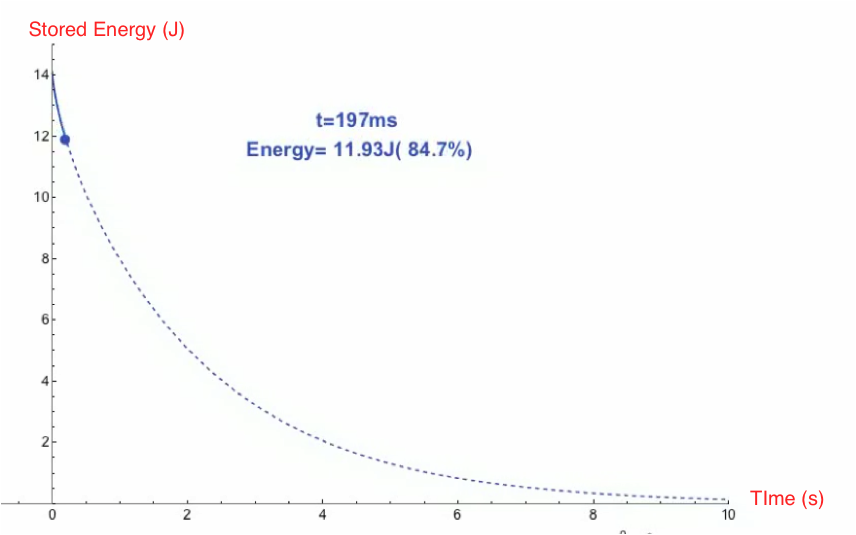
\includegraphics[width=0.7\textwidth,trim=2mm 2mm 2mm 2mm,clip]{A2r} \\ \vspace{20pt}    %update image with red labels, trim border
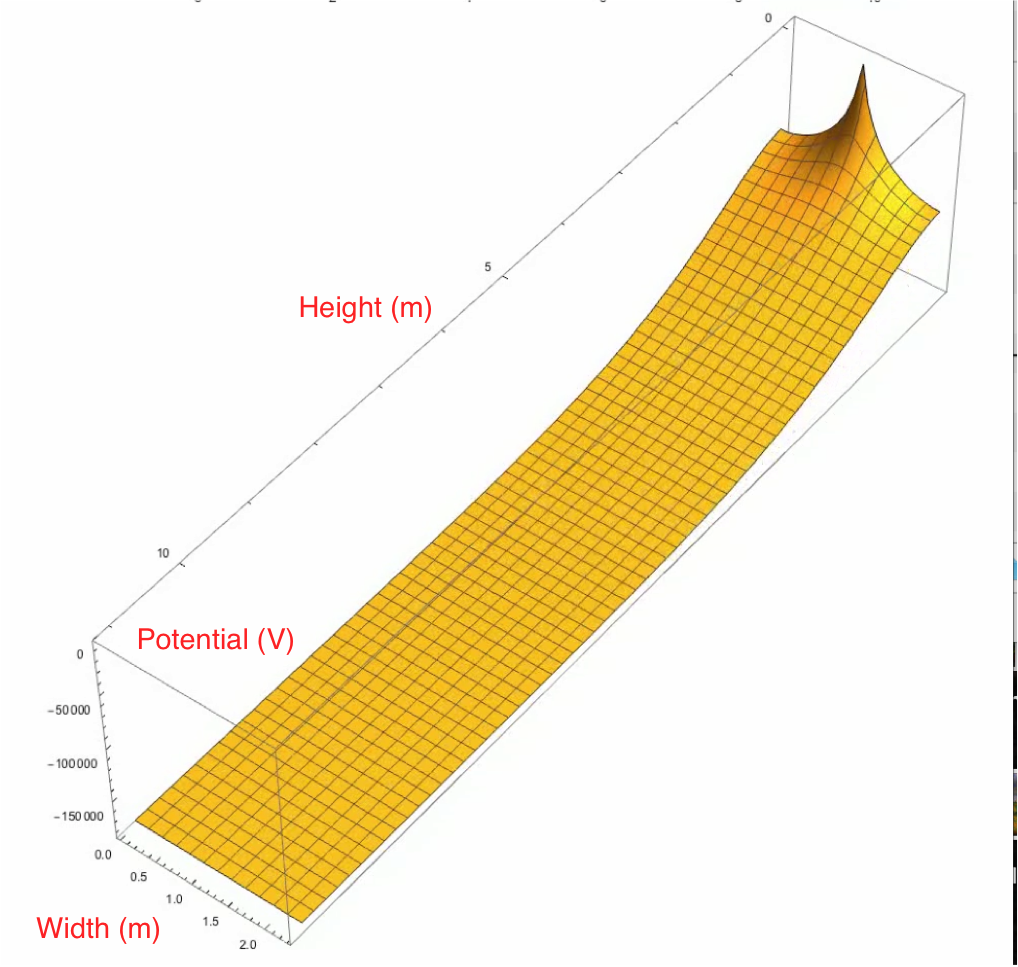
\includegraphics[width=0.6\textwidth,trim=2mm 2mm 2mm 2mm,clip]{A3r}
\end{dunefigure}

%The \single \dword{hv} system may have modifications if problems are identified in the present design in \dword{pdsp}. 


%%%%%%%%%%%%%%
\subsubsection{Structural Considerations}

The frames around the \dword{cpa} panels and the frames supporting the \dword{fc} aluminum profiles  
are made from materials with similar thermal expansion coefficients, minimizing issues of differential thermal expansion. The \dword{fc} frames 
are restrained at only one location.  
%Cold testing of a \dword{cpa}, with monitoring of its geometry and electrical resistance is documented in DocDB 2338. In addition, Docdb 1504 documents the testing at cryogenic temperatures of kapton/\frfour laminates and the shrinkage of the detector was examined in Docdb 6011.
%Each \dword{topfc} and \dword{botfc} module is nominally \SI{2.3}{\m} wide by  \SI{3.5}{\m} long (along the \dword{detmodule} length). 

The \dwords{cpa} and \dwords{apa} support the \dword{topfc} and \dword{botfc} modules, whereas
%The \dword{topfc} and \dword{botfc} modules are supported by the \dwords{cpa} and \dwords{apa}. 
%The \dwords{ewfc} modules are \SI{1.5}{\meter} tall by \SI{3.5}{\meter} long. They are stacked eight units high to cover the \SI{12}{\meter} height of the \dword{tpc}.  
installation rails above the \dwords{apa} and \dwords{cpa} support the \dword{ewfc} modules. 
%are supported by the installation rails above  the \dwords{apa} and \dwords{cpa}, which are part of the \dword{dss}. 

All structural members of the CPAs and FCs are made of either FR4 or FRP with very similar CTEs. However, the structures supporting the CPAs and FCs are made of stainless steel, whose CTE is about 50\% greater.  To accommodate the mismatch in the CTEs, small expansion gaps are added between CPAs at the installation time.  These gaps are expected to disappear at the operating temperature.
 
%%%%%%%%%%%%%%
\subsubsection{Design Validation}

Extensive testing has %been performed of 
validated the mechanical and electrical properties of materials selected for the \dword{hv} system.  These are fully documented in references ~\cite{bib:docdb2338, bib:docdb1504, bib:docdb1601}.
%\fixme{ Already there! Add to bib: \textit{CPA Electrical Connections Cold Test}, DUNE DocDB 2338; \textit{CPA and FC Design}, DUNE DocDB 1504; \textit{Technical Review: Mechanical Specifications for \dword{pdsp} \dword{fc} test in \dword{35t} at \fnal}, DUNE DocDB 1601.}

Issues identified in earlier testing form the basis of an ongoing R\&D program. 


Operation experience from \dword{pdsp} is summarized in Section \ref{sec:fdsp-hv-protodune}. It revealed some instabilities in the HVS operations.  Design changes (see Section \ref{sec:fdsp-hv-des-fc-gp}) have been introduced to the top and bottom field cage assemblies to further decrease the overall electric field between the profiles and the ground planes.


%%%%%%%%%%%%%%%%%%
\subsection{HV System Safety}
\label{fdsp-hv-design-safety}

%Safety is central to the design of the \dword{hv} system. In all phases including fabrication, installation, and operations, safety will be the highest priority. There will be documented assembly, testing, transport, and installation procedures. Particular attention was paid to these topics in the design of  \dword{pdsp}  with explicit concern to a design that is identical to the \dword{spmod} design, the most critical of which are also noted in the preliminary \dword{hv} risk assessment, which is under development. %Commented for IDR -\fixme{ref properly. RKP: Requires reference policy, under discussion.}

Safety is central to the design of the \dword{hv} system and is the highest priority concern in all phases: fabrication, installation, and operations. Documentation of assembly, testing, transport, and installation procedures is in progress. Particular attention was paid to these procedures in the design of \dword{pdsp}, with the explicit understanding that they be applicable to the \dword{spmod}. The most critical procedures are also noted in the preliminary \dword{hv} risk assessment, which is under development. %Commented for IDR -\fixme{ref properly. RKP: Requires reference policy, under discussion.}

The structural and electrical designs for the \dword{spmod} \dword{hv} are closely modeled on designs that were vetted and validated in the \dword{pdsp} construction. 
%\fixme{IOW, the designs are not the same, but are based on the \dword{pdsp} designs?}
Previous to \dword{pdsp}, Fermilab tested a full-voltage and full-scale \dword{hv} feedthrough, power supply, filtering, and monitoring system, along with the \dword{hv} connection cup and arm (described in Section???), after completing full safety reviews. These devices worked as designed and are essentially reproduced in both \dword{pdsp} and the \dword{spmod}. 

%When operating the \dword{fc} at its full operating voltage there is a substantial amount of stored energy. 
At full operating voltage the \dword{fc} stores a substantial amount of energy.
%The design of the \dword{cpa} is centered around storing charge  at the highest voltage on a resistive surfaces to limit the power dissipated during a power supply trip or other failure which unexpectedly drops the \dword{hv}. 
As discussed in Section~\ref{sec:fdsp-hv-des-elec}, the \dword{cpa} is designed to limit the power dissipated during a power supply trip or other failure that unexpectedly drops the \dword{hv}.
Its design has succeeded in tests at full voltage over \num{2}\,m$^2$ surfaces and at larger scale in \dword{pdsp}.  

Integral to the \dword{pdsp} and \dword{spmod} design is the concept of pre-assembled modular panels of field-shaping conductors with individual voltage divider boards. The structural design and installation procedures used in \dword{pdsp} were selected to be compatible with use at the \dword{fd} site and were vetted by project engineers, engineering design review teams, and CERN's safety engineers. Any revisions to these designs based on lessons learned in \dword{pdsp}  installation and operations will be reviewed both within the project and by Fermilab \dword{esh} personnel. The safety features of the overall design are on solid footing. 



%%%%%%%%%%%%%%%%%%%%%%%%%%%%%%%%%%%%%%%%%%%%%%%%%%%%%%%%%%%%%%%%%%%%
%\section{HV System Design}
%\label{sec:fdsp-hv-design}

%%%%%%%%%%%%%%%%%%%%%%%%%%%%
\section {HV Power Supply and Feedthrough}

The \dword{hv} delivery system consists of
\begin{itemize}
\item two power supplies,
\item \dword{hv} cables,
\item filter resistors, and
\item \dword{hv} feedthroughs into the cryostat.
\end{itemize}

For \dword{hv} delivery, two power supplies generate the voltage, one for each \dword{cpa} array. 
This separated setup more easily accommodates different running conditions and helps isolate any instabilities. 
The cryostat design has two feedthrough ports for each \dword{cpa} array, one at each end of the cryostat. The spare downstream port provides redundancy against any failure of the primary \dword{hv} delivery system. 
%In the event only one power supply is available, the system will be run by using a \dword{hv} splitter outside of the cryostat while another power supply is procured. 

Each \dword{cpa} array 
services two drift volumes in parallel, 
presenting a net resistance of \SI{1.14}{\giga\ohm} to each power supply. At the nominal \SI{180}{kV} cathode voltage, each power supply must provide \SI{0.16}{mA}.

The power supply model planned for the \dword{spmod} is similar to that used on \dword{pdsp}.\footnote{Heinzinger, PNC HP300000 \dword{hv} power supply, Heinzinger\texttrademark{} Power Supplies, \url{http://www.heinzinger.com/}.}  %, with a maximum output voltage of \SI{200}{kV} and a maximum current draw of \SI{0.5}{mA}.  
Another %additional 
option being considered is a \SI{200}{kV}, \SI{0.5}{mA} model from the same vendor. 
The \dword{hv} cables are commercially available models compatible with the selected power supplies. 

%The \dword{hv} cables will be either Dielectric Sciences model number 2134 capable of \SI{200}{kV} DC or 2236 capable of \SI{320}{kV} DC. 
%ielectrThe \dword{hv} cables are preferred to be Dielectric Sciences model number 2134 capable of \SI{200}{kV} DC.  A back up plan is to use model 2236 capable of \SI{320}{kV} DC. 

Filter resistors  are placed between the power supply and the feedthrough.  Along with the cables, these resistors reduce the discharge impact by partitioning the stored energy in the system.  The resistors and cables together also serve as a low-pass filter reducing 
the \SI{30}{kHz} voltage ripple on the output of the power supply.  With filtering, such supplies have been used successfully in other \lartpc experiments, such as \microboone and ICARUS.Figure~\ref{fig:ps_filter_ft_schematic} shows the \dword{hv} supply circuit.

\begin{dunefigure}[A schematic showing the \dword{hv} delivery system to the cryostat.]  
{fig:ps_filter_ft_schematic}
{Left: Examples of \SI{300}{kV} and \SI{200}{kV} power supplies. %An example 
 (Credit: CERN). Right:  A schematic showing the \dword{hv} delivery system to the cryostat. (Credit:  SEL).  
One of the two filter resistors sits near the power supply; the other sits near the feedthrough.}
%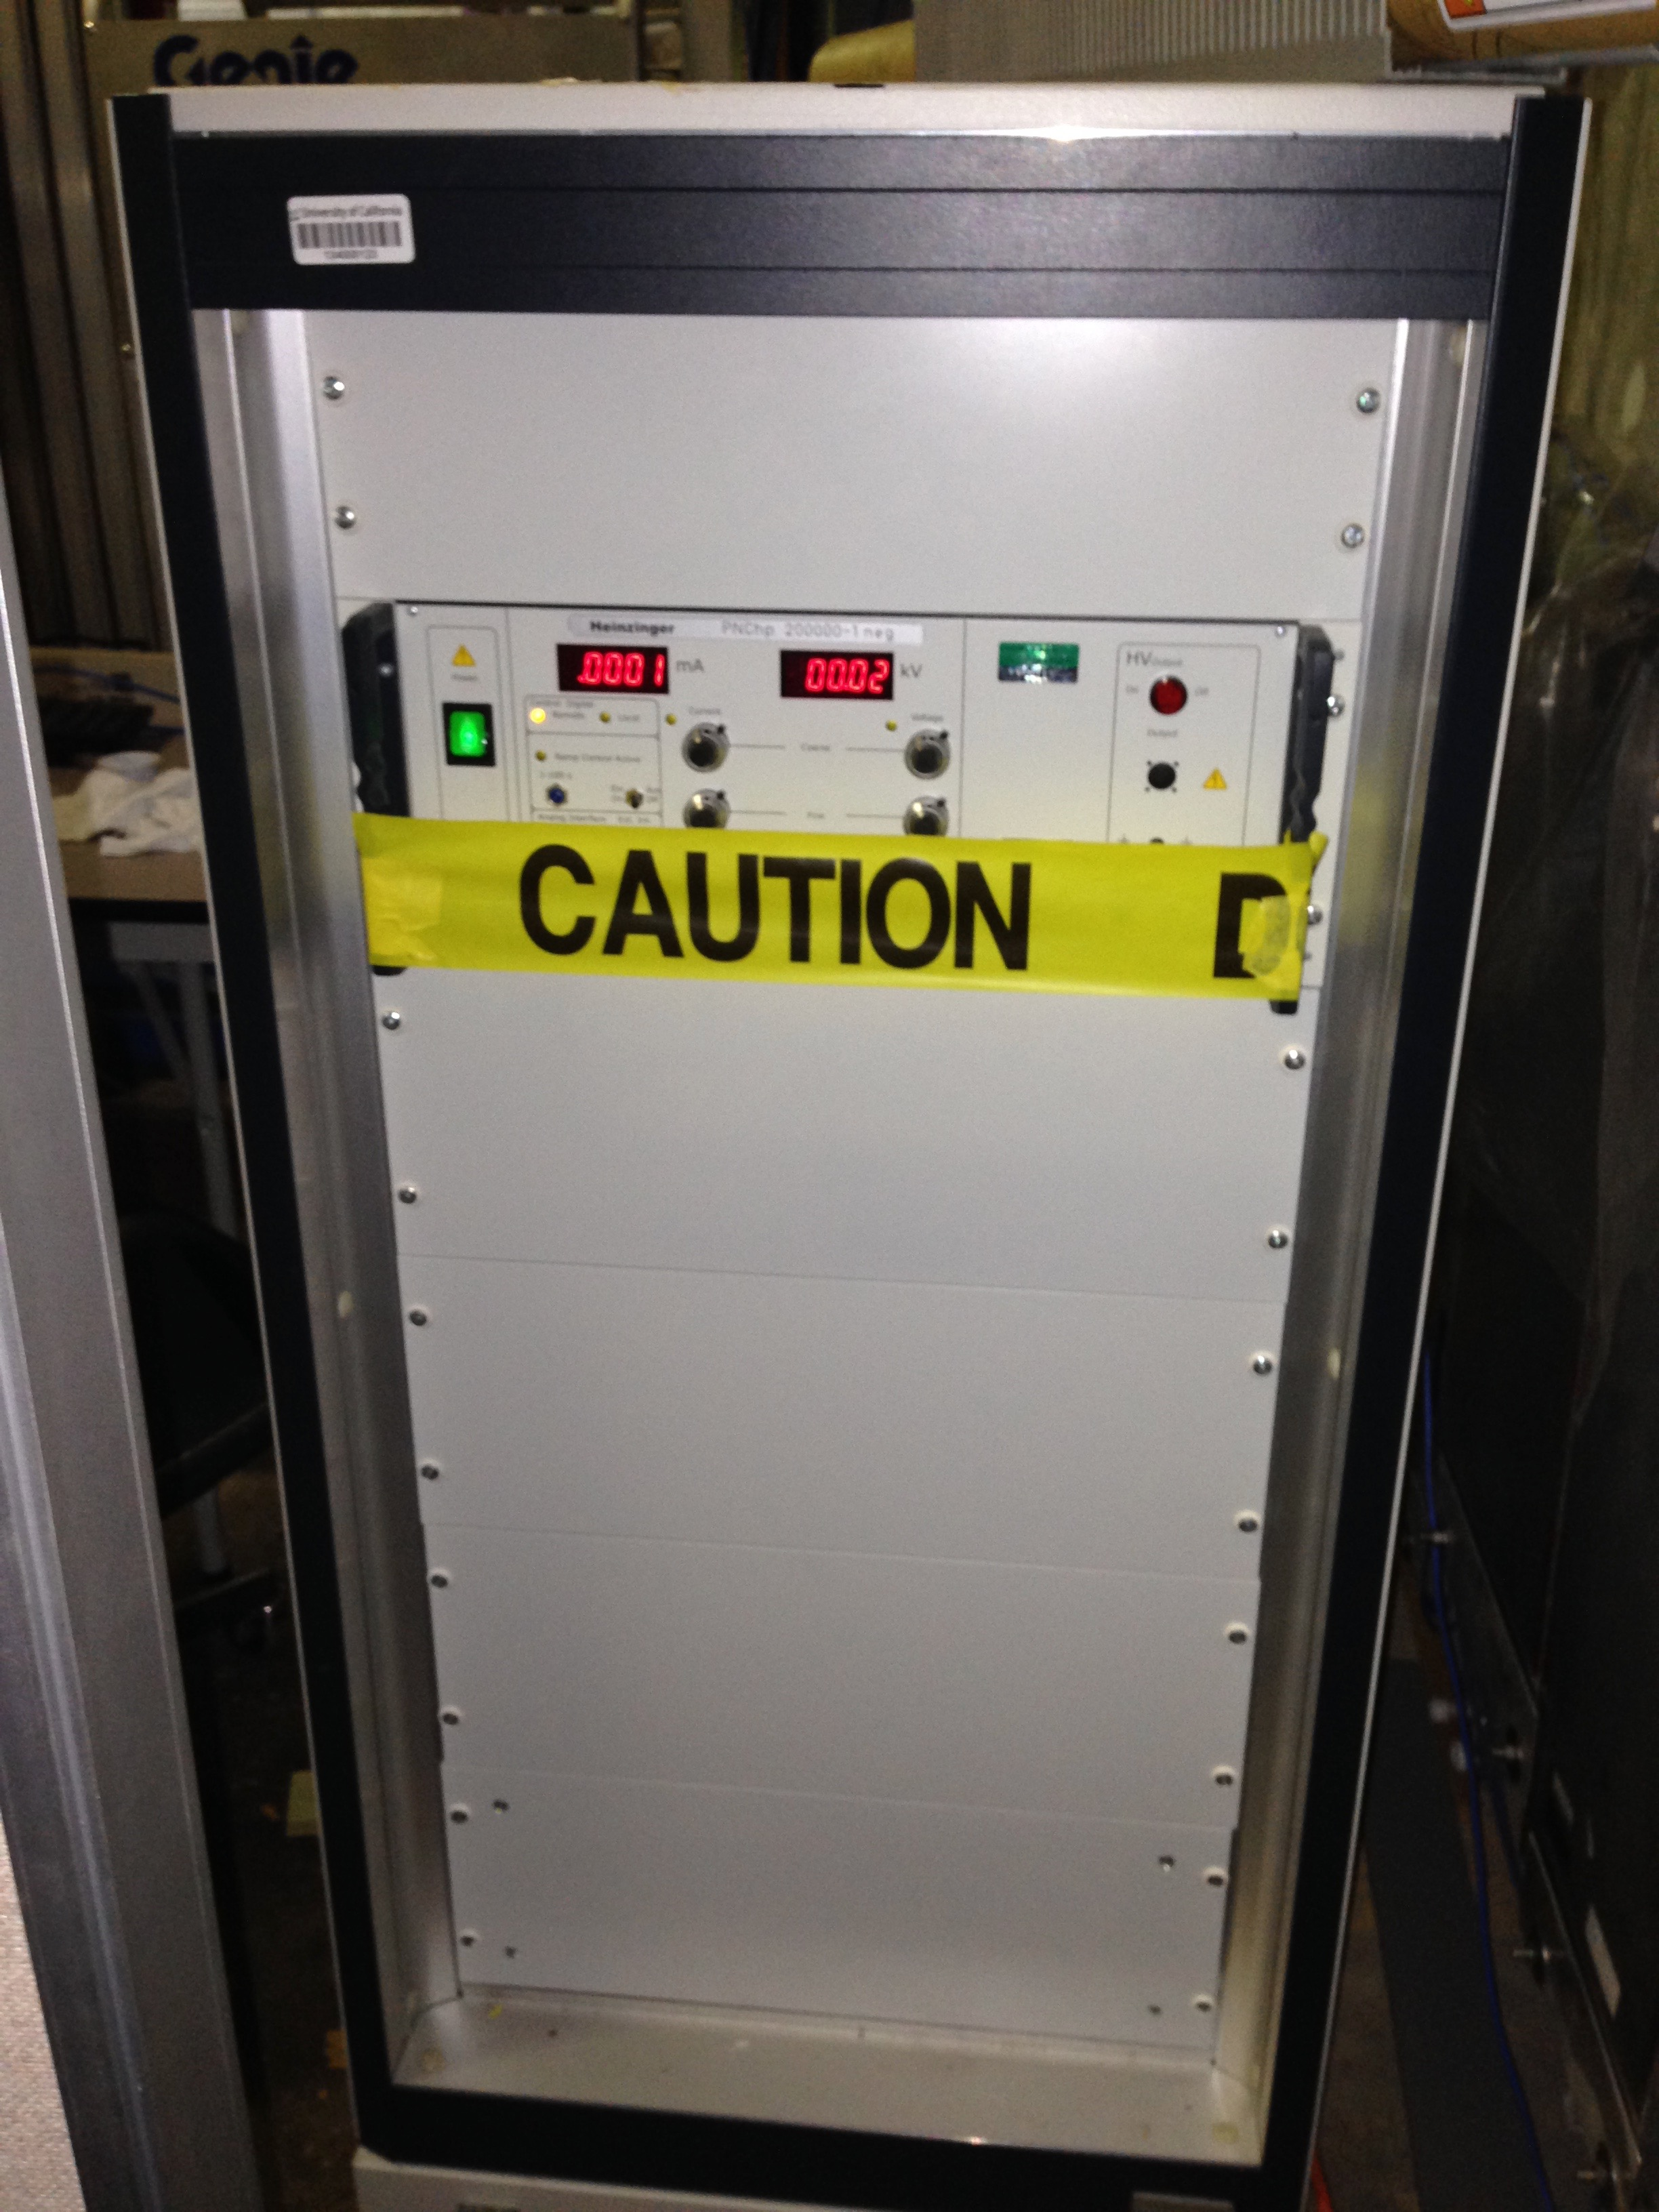
\includegraphics[width=0.2\textwidth]{heinzy}
%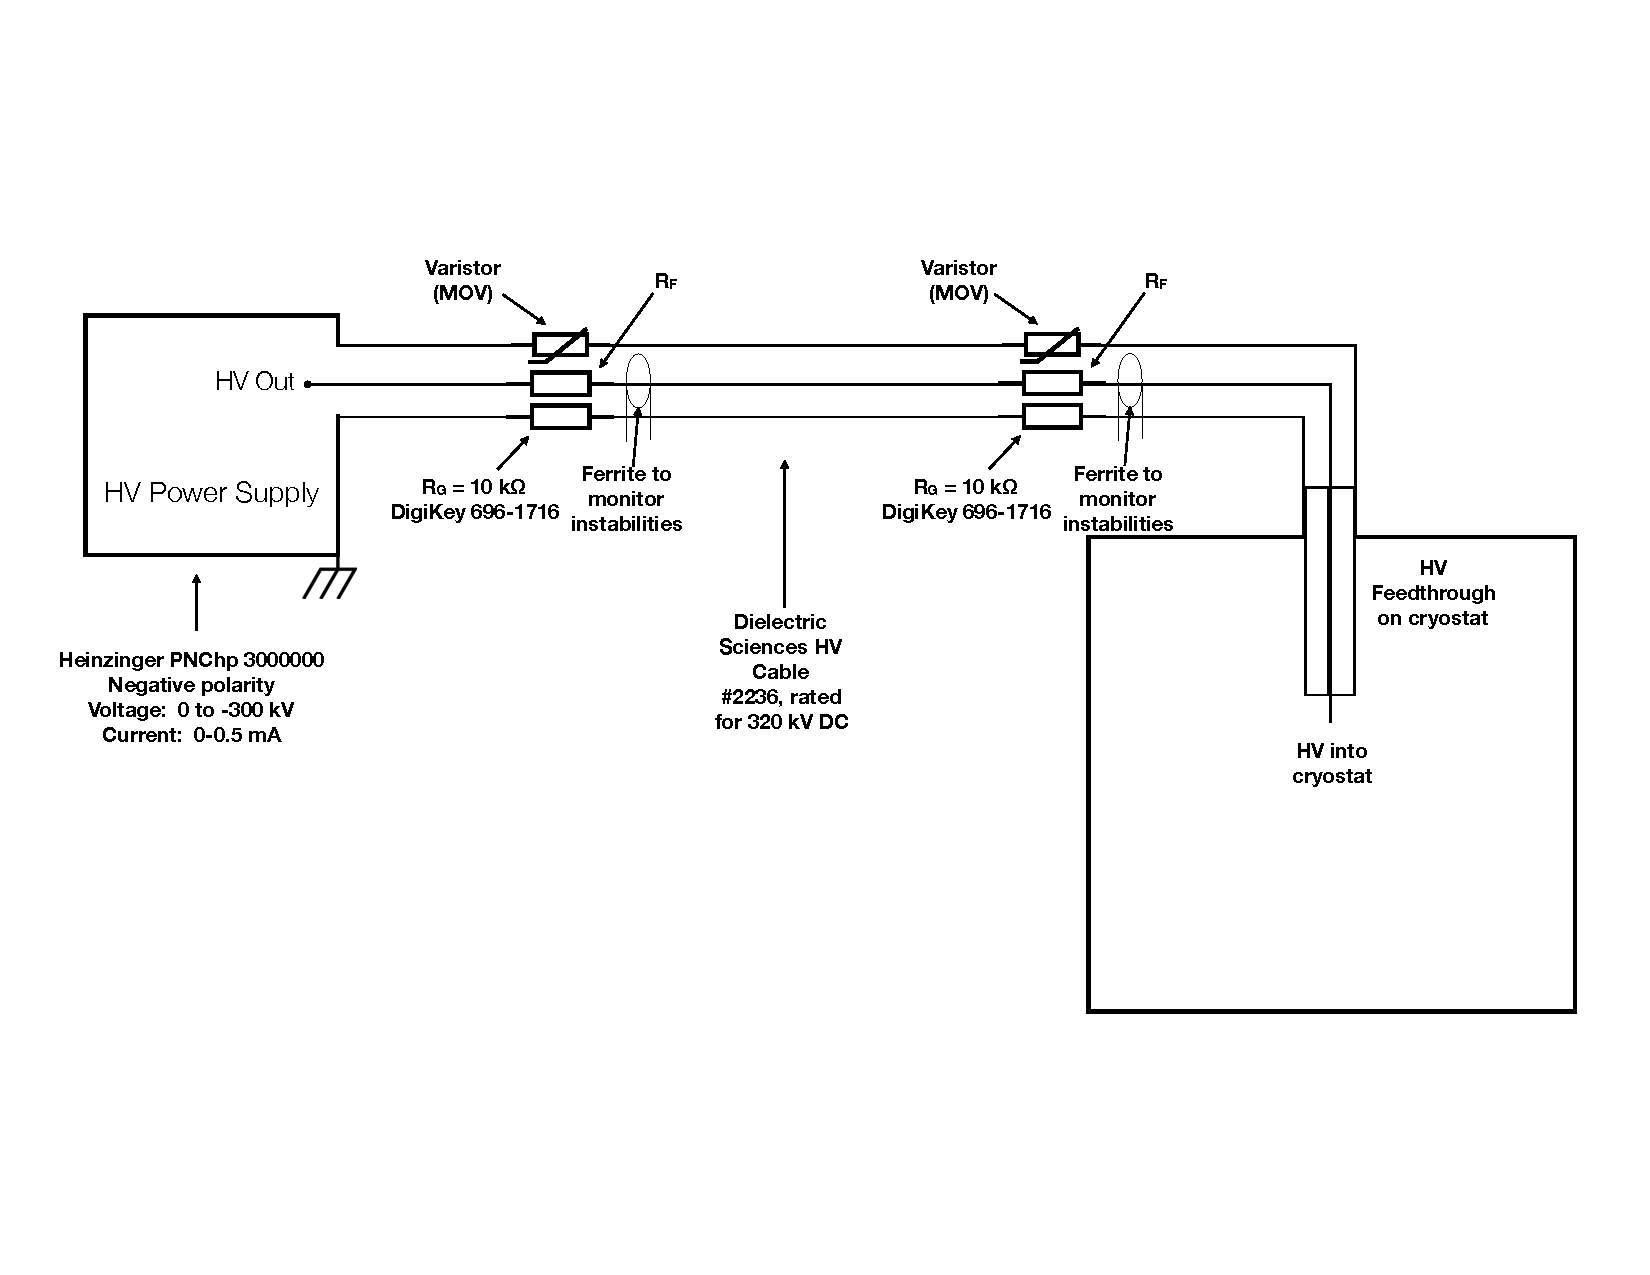
\includegraphics[width=0.7\textwidth]{ps_filter_ft_schematic}  %requested image edits by DeMuth
\begin{minipage}{\textwidth}%{6in}
  \centering
 $\vcenter{\hbox{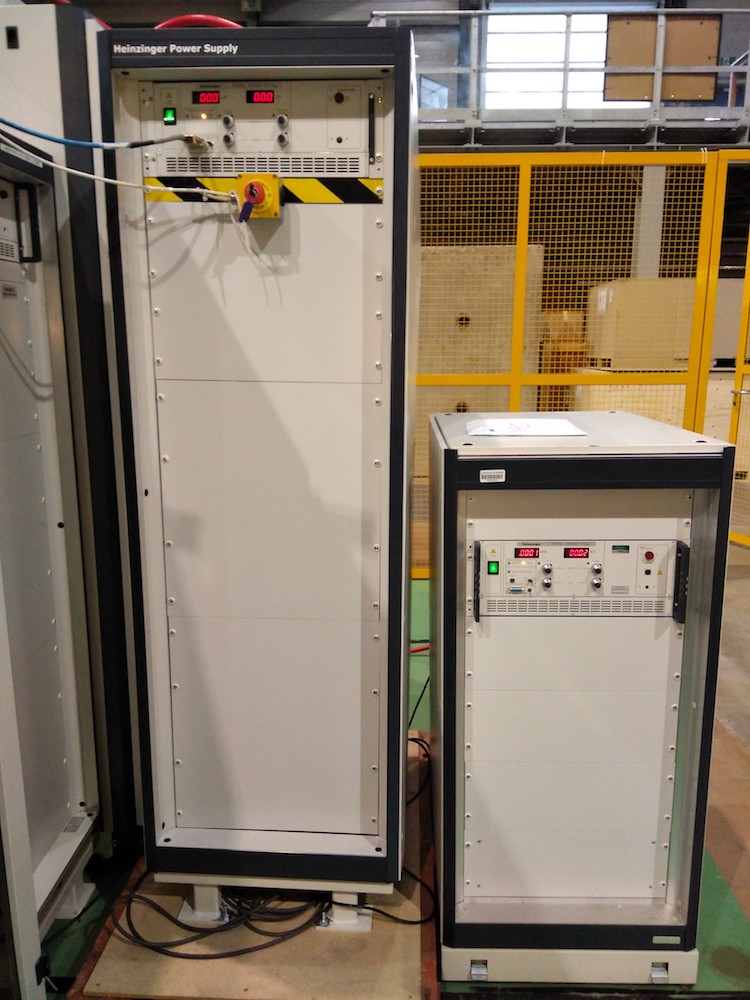
\includegraphics[width=0.2\textwidth]{Power_Supplies_300_and_200.jpg}}}$
 \hspace*{0.001\textwidth}  $\vcenter{\hbox{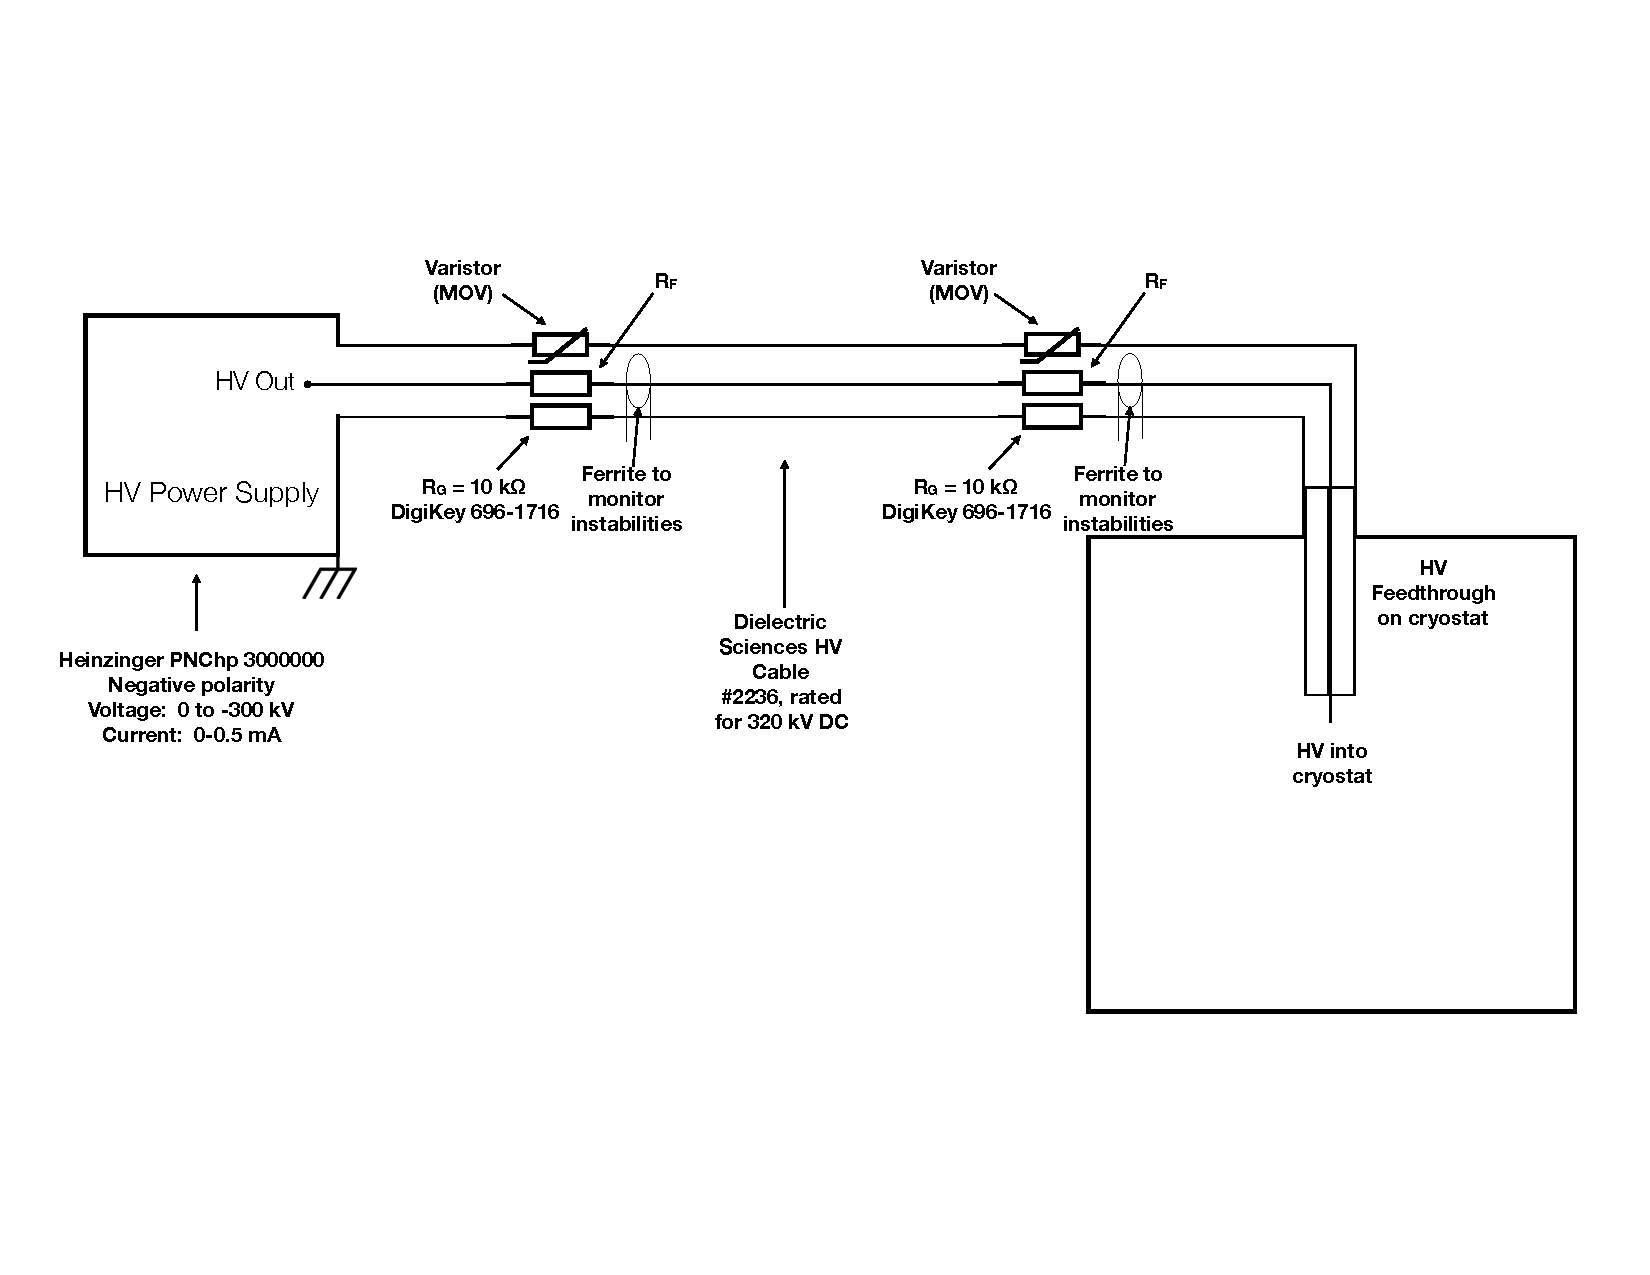
\includegraphics[width=0.75\textwidth]{ps_filter_ft_schematic}}}$
\end{minipage}
\end{dunefigure}
The requirement  
on low electronics noise sets the upper limit of residual voltage ripple on the cathode to be \SI{0.9}{mV}. 
%\fixme{specs sheet says: \hvripplenoise} 
Typically, commercial supplies specify a ripple variation limit of 
\SI{.001}{\%} around an absolute precision in nominal voltage of $\pm$\SI{50}{mV}.
%
Assuming cable lengths of \SI{30}{m} and \SI{3}{m} between the filters themselves, and between the filter and \fdth, respectively, calculations and experience confirm that resistances as low as a few \si{\mega\ohm} yield the required noise reduction. 

The %current plan for the 
filter resistors are of a cylindrical design. 
Each end of a \dword{hv} resistor is electrically connected to a cable receptacle. 
The resistor %should shall be selected to 
must withstand a large over-power condition.  Radially out from the resistor is an insulator. %,  for which other designs have used transformer oil or \dword{uhmwpe}. 
%\fixme{ultrahigh molecular weight. polyethylene . one acronym}
The outer case of the filter is a grounded stainless steel or aluminum shell. The filter design used for \dword{pdsp} is shown in Figure~\ref{fig:filterAndFeedthrough}.

The \dword{hv} feedthrough %will be 
is based on the successful ICARUS design \cite{ICARUS-t600}, %\fixme{reference to S. Amerio et al., Nuclear Instruments and Methods in Physics Research A 527 (2004) 329 - 410, already available in tdr-citedb as ICARUS-t600} 
which was adapted for \dword{pdsp}.  The voltage is transmitted by a stainless steel center conductor.  On the warm side of the cryostat, this conductor mates with a cable end.  Inside the cryostat, the end of the center conductor has a spring-loaded tip that %will 
contacts a receptacle cup mounted on the cathode, delivering \dword{hv} to the \dword{fc}.  The center conductor of the \fdth is surrounded by ultra-high molecular weight polyethylene (\dword{uhmwpe}), an insulator. This is illustrated in Figure~\ref{fig:filterAndFeedthrough}.

\begin{dunefigure}[Drawings of the \dword{hv} filters and feedthroughs]{fig:filterAndFeedthrough}
{  Photograph and drawing of a \dword{hv} \fdth (Credit:  F.~Sergiampietri).}
%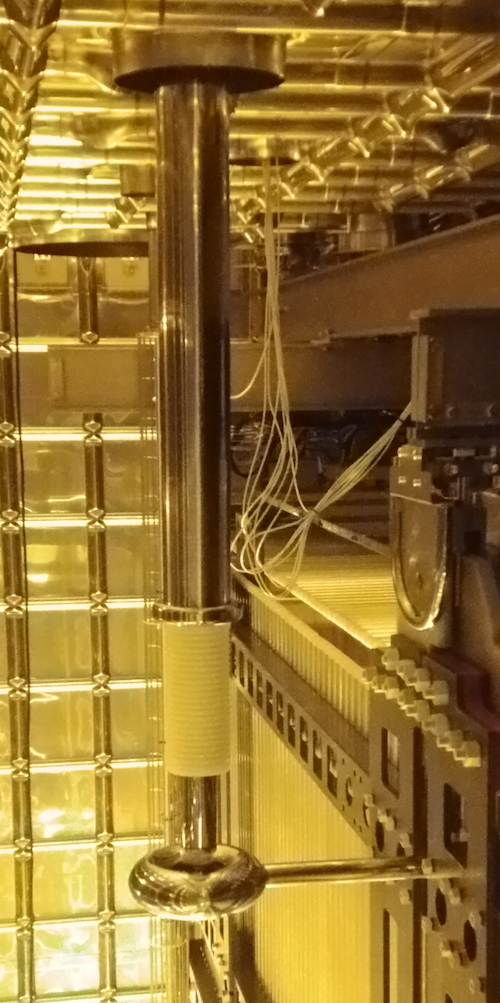
\includegraphics[width=0.15\textwidth]{hv_feedthrough.png}
%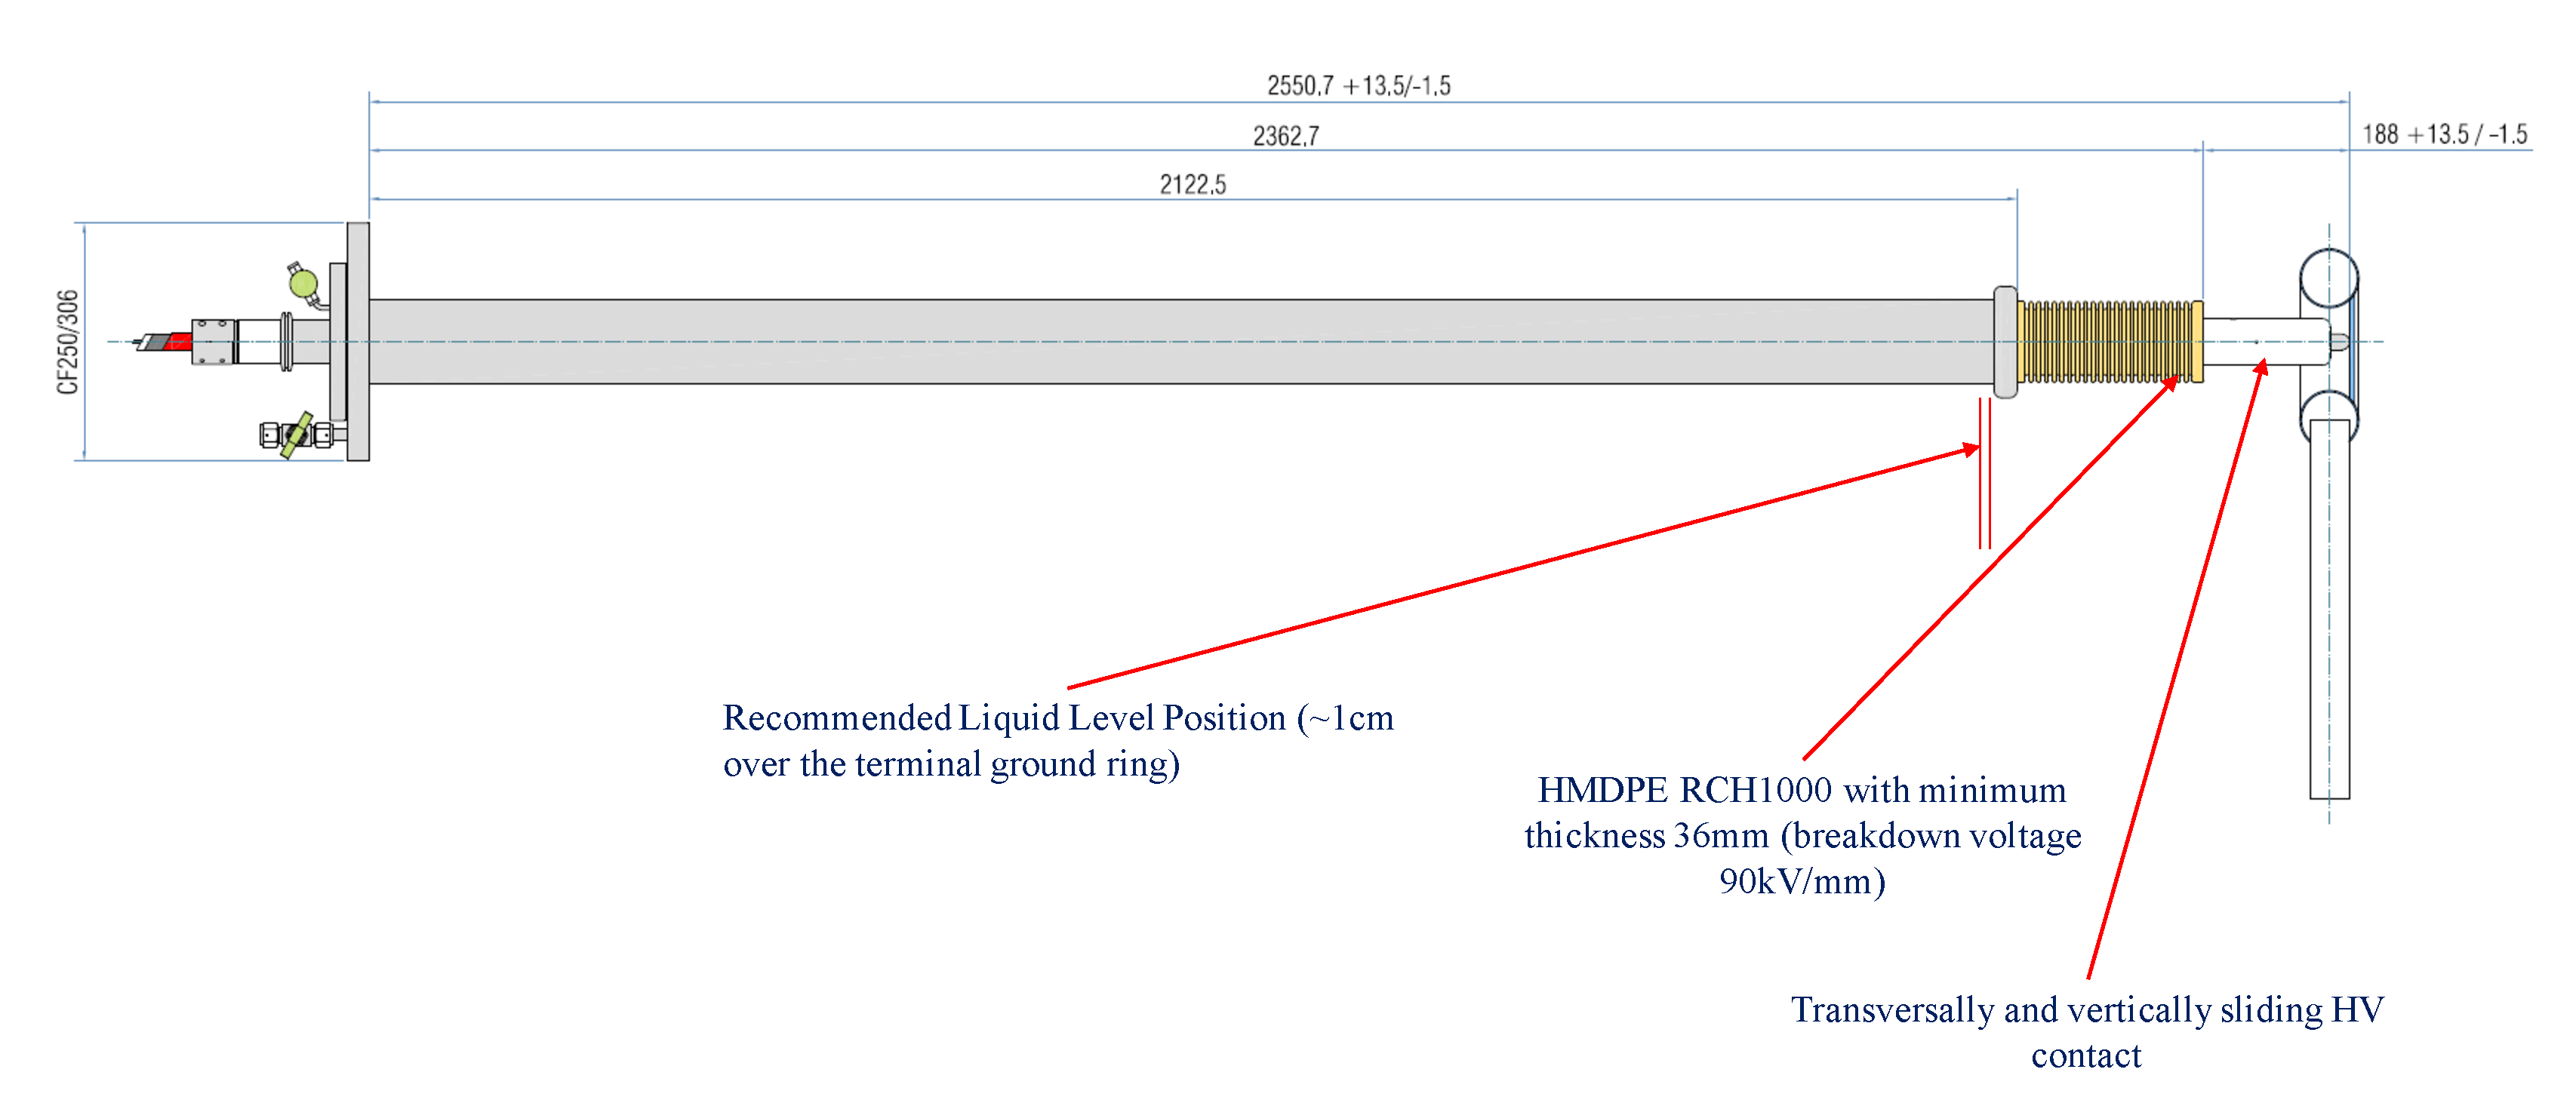
\includegraphics[width=0.8\textwidth]{francosHVFT}
\begin{minipage}{\textwidth}%{6in}
  \centering
 $\vcenter{\hbox{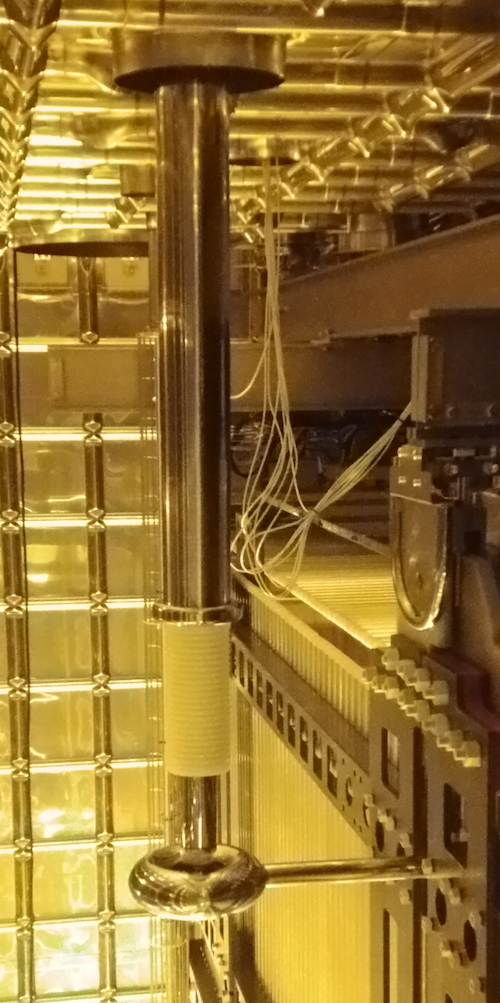
\includegraphics[width=0.12\textwidth]{hv_feedthrough.png}}}$
 \hspace*{0.001\textwidth}  $\vcenter{\hbox{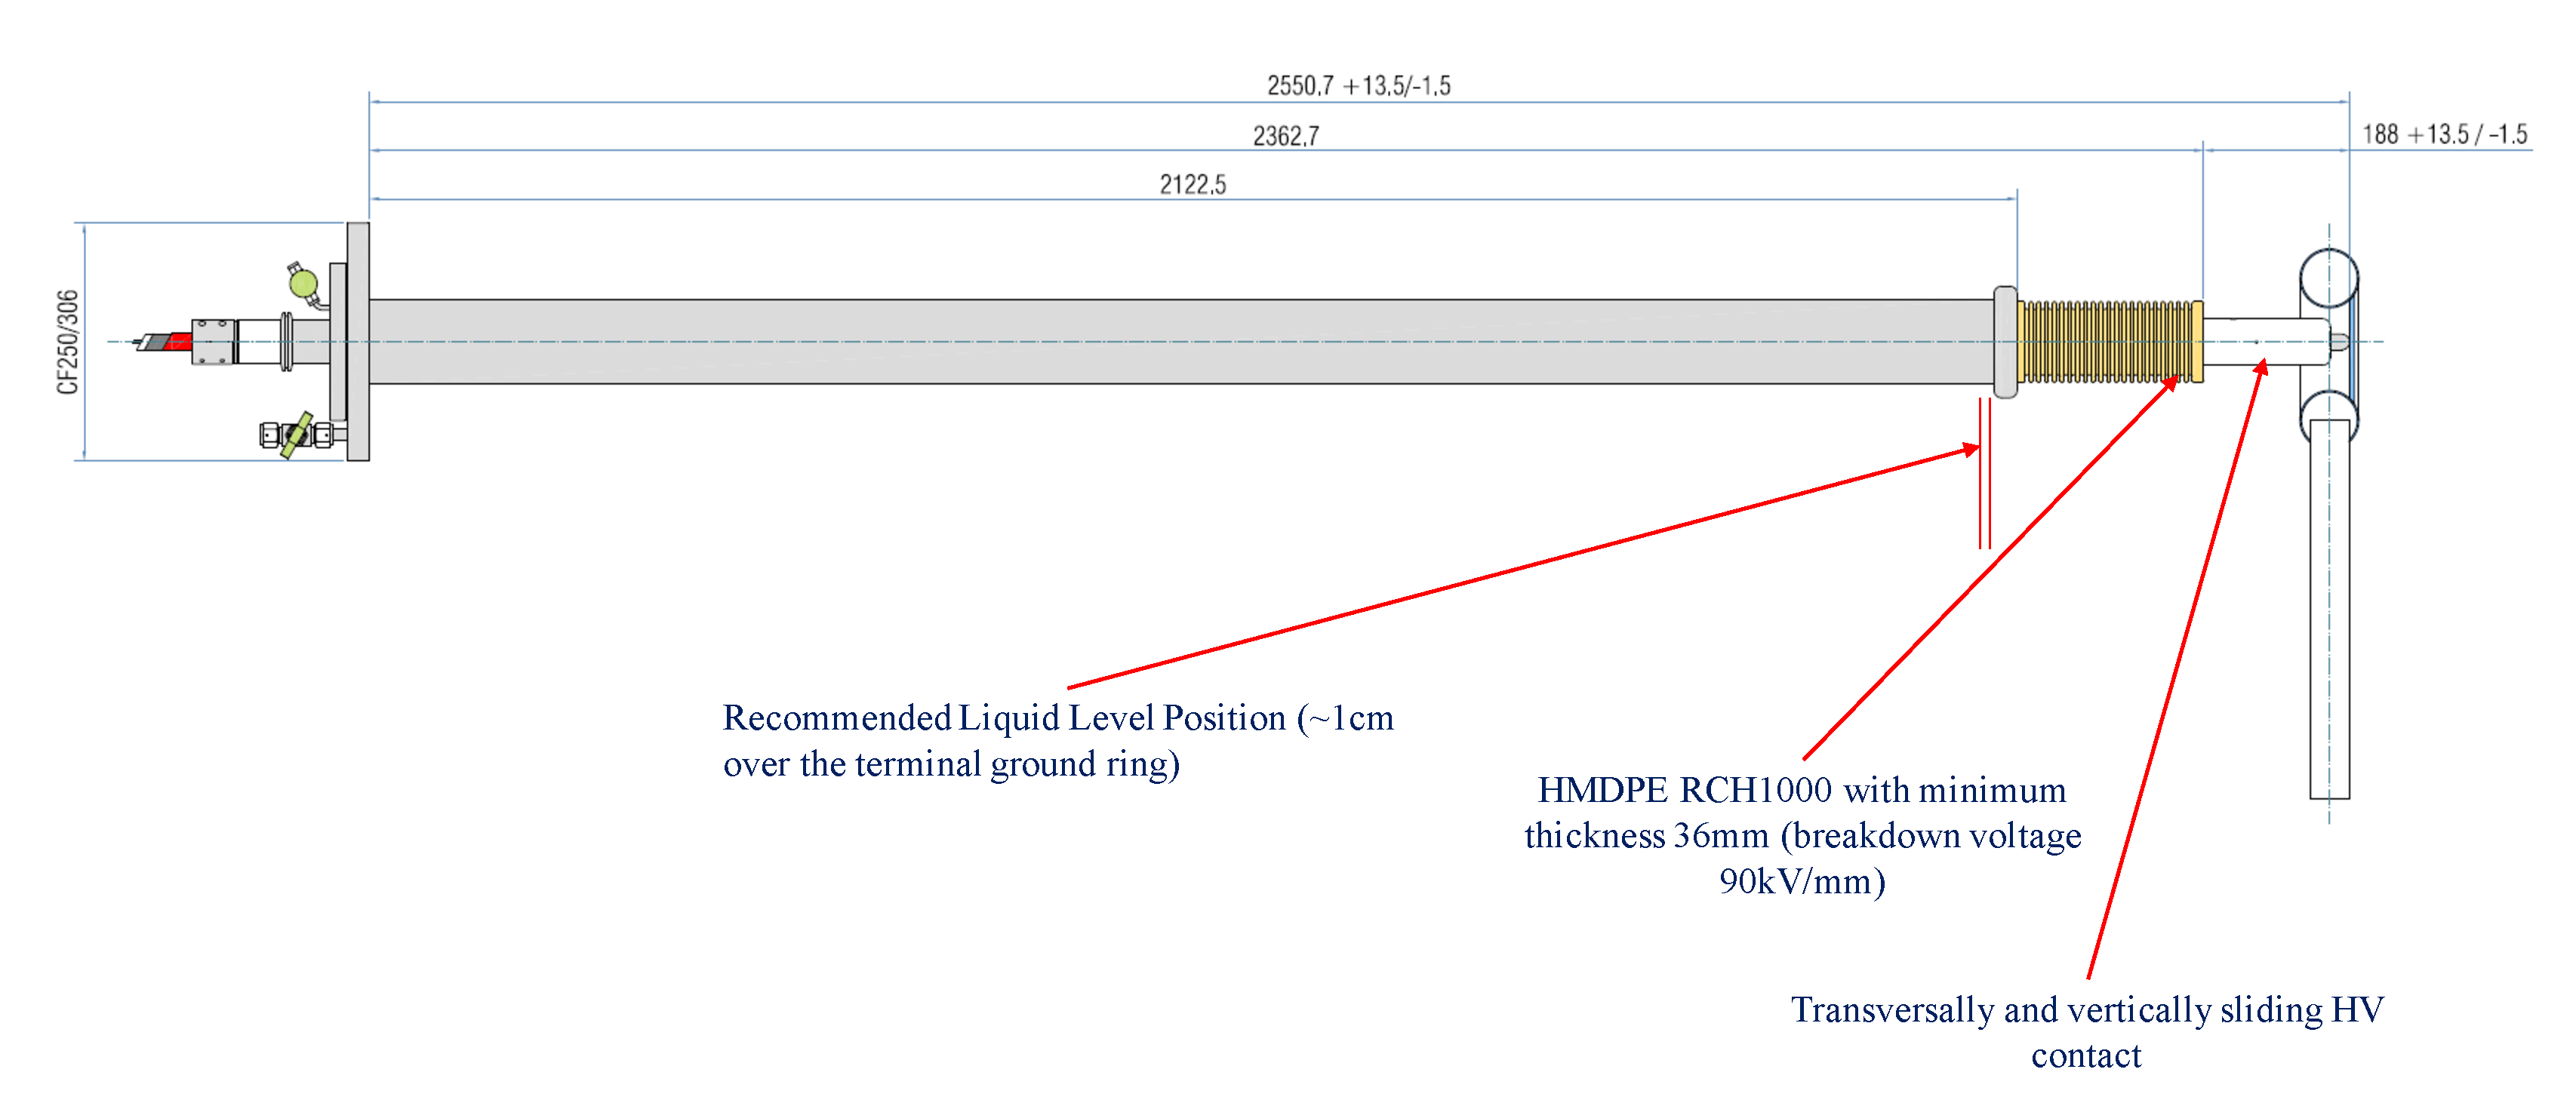
\includegraphics[width=0.86\textwidth]{francosHVFT}}}$
\end{minipage}
\end{dunefigure}

To first order the operating voltage upper bound on a feedthrough is set by the maximum \efield{} on it. %the feedthrough.  
This \efield{} is reduced by increasing the insulator radius.  For the target voltage, the feedthrough uses a \dword{uhmwpe} cylinder of approximately \SI{15}{cm} diameter.  In the gas space and into at least \SI{15}{\centi\meter} of the liquid, the insulator is surrounded by a tight-fitting stainless steel ground tube.  A %\SI{25}{\centi\meter}  
Conflat industry standard flange is welded onto the ground tube for attachment to the cryostat.

Outside the cryostat, the \dword{hv} power supply and cable-mounted toroids monitor the \dword{hv}.    The power supplies 
have capabilities down to tens of \si{\nano\ampere} in current read-back 
and are able to sample the current and voltage every \SI{300}{\ms}.  The cable-mounted toroids are sensitive to fast changes in current;  
the polarity of a toroid's signal  
indicates the location of the current-drawing feature as either upstream or downstream of it.  Experience from the DUNE \dword{35t} installation suggests that sensitivities to changing currents %with 
are on a timescale between \SIrange{0.1}{10}{\micro\s}.

Inside the cryostat, pick-off points near the anode monitor the current  
in each resistor chain.  Additionally, the voltage of the \dwords{gp} above and below each drift region can be equipped to diagnose problems via a high-value resistor connecting the \dword{gp} to the cryostat.  In the DUNE \dword{35t}, such instrumentation provided useful information on \dword{hv} stability and locations of %where 
any stray charge flows. %was flowing.

Both commercial and custom \dword{hv} components must be rated for sufficient voltage and satisfy tests to meet the specifications %requirements 
summarized in Section \ref{sec:fdsp-hv-des-consid}.  Further details on these tests are in Section \ref{sec:fdsp-hv-transport-QC}.

The resistances in the filters, in combination with the capacitances between the \dword{hv} system and the cathode,
 determine the attenuation of the tens of \si{\kilo\hertz} ripple from the power supply.  The filters  
are designed such that the ripple is reduced to an acceptable level when installed in the complete system, thus satisfying specification %requirement 
TOP-12 
%in Table~\ref{tab:spec:hv-ps-ripple} %(3) 
that the power supply ripple be negligible. %minimized.
%\fixme{Need to fix names of requirements; TOP-12 is not very elegant. Anne}

%%%%%%%%%%%%%%%%%%%%%%%%%%%%
\section{CPA Arrays}

Two vertical, planar \dword{cpa} arrays held at \dword{hv} each provide constant-potential surfaces at \SI{-180}{\kV} for a \dword{spmod}. Each \dword{cpa} array also distributes \dword{hv} to the first profile on the top and bottom \dword{fc} and to the \dwords{ewfc}. The configuration of the \dword{cpa} arrays is described in Section~\ref{sec:fdsp-hv-des-cpa}.
%\fixme{In table 1.4 we have top and bottom fc modules. Are these elements different from modules? Anne. RKP-removed element}

Resistive panels (RPs) form the constant-potential surfaces of each \dword{cpa} unit. The \dwords{rp} are  composed of a thin layer of carbon-impregnated Kapton\footnote{DuPont\texttrademark{}, Kapton\textsuperscript{\textregistered} polymide film,  E. I. du Pont de Nemours and Company,  \url{http://www.dupont.com/}.} laminated to both sides of a \SI{3}{\milli\meter} thick \frfour sheet of \SI{1.2}{\meter}  $\times$ \SI{2}{\meter} size.  

A \dword{cpa} array receives its \dword{hv} via the feedthrough that makes contact with the \dword{hv} bus mounted on the \dword{cpa} frame through a cup assembly attached to the frame, as shown in Figure~\ref{fig:cup_cpa}. 
One cup assembly attaches to each end of the two \dword{cpa} arrays, for a total of four. Details on the electrical connections are in Section~\ref{sec:fdsp-hv-design-interconnect}.

\begin{dunefigure}[HV input connection to \dword{cpa} array]{fig:cup_cpa}{\dword{hv} input cup connection to \dword{cpa} array.}
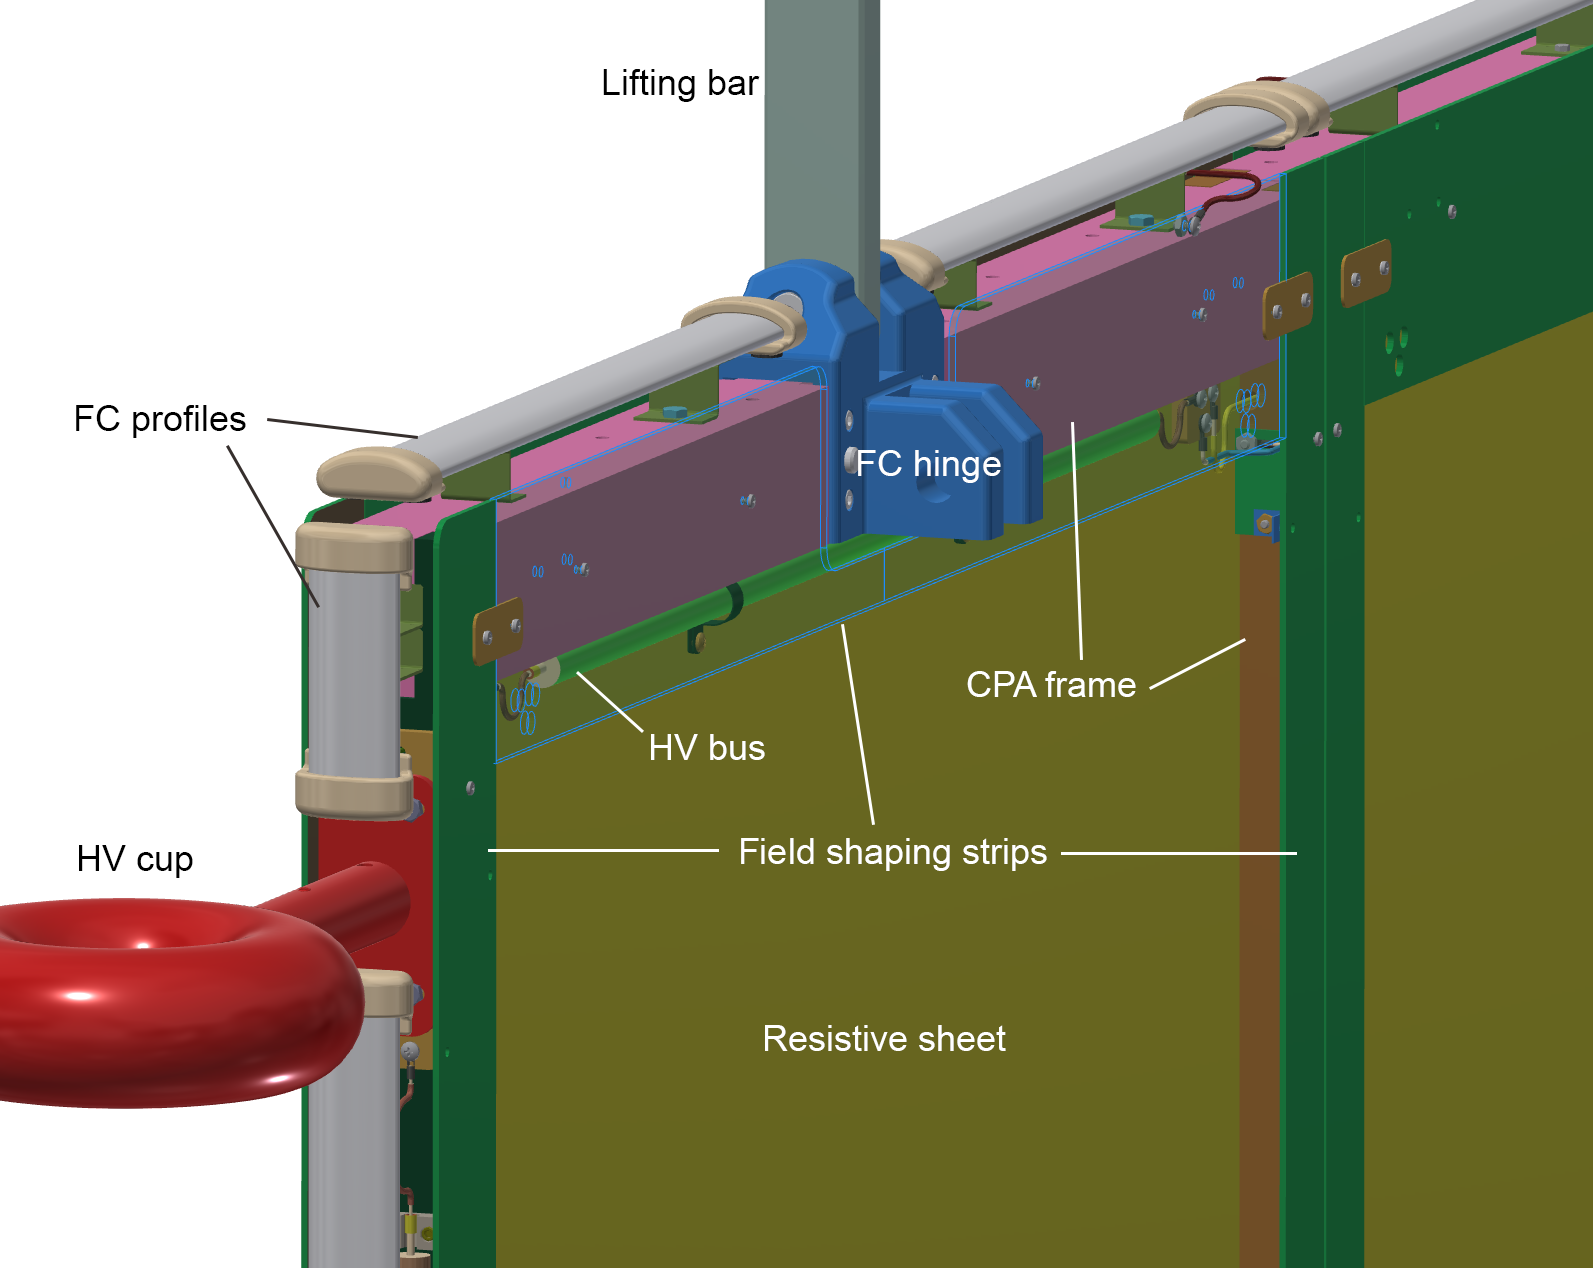
\includegraphics[width=0.6\textwidth]{donut_cpa2} %{ was Latest3D}
\end{dunefigure}

In accordance with specification TOP-17,
the surface resistivity of the \dwords{rp} is required to be greater than \cathodemegohm to provide for slow reduction of accumulated charge in the event of a discharge.  Given the anticipated higher stored energy at the \dword{fd} 
relative to the prototypes, we set a goal of \cathodegigohm to further  protect against potential discharges.  
 
To maintain the position and flatness of the cathode, 
\SI{6}{cm} thick \frfour frames are placed at \SI{1.2}{m} intervals between the \dword{cpa} panels. This design ensures the cathode distortion caused by a small pressure differential (up to about \SI{1}{Pa}) across the cathode surface from the convective flow of the \lar is within spec. 
%% last sentence modified by BY

The \dword{cpa} frames are required to support, in addition to the \dword{hv} components, the \dword{topfc} and \dword{botfc} units attached to both sides of the \dword{cpa} plane. %plane. 
The arrangement and deployment of these components is identical to that in \dword{pdsp}.  

 Since \frfour is a good insulator at cryogenic temperatures with a dielectric constant different from that of \lar, the presence of the \dword{cpa} Panel frames causes a local \efield distortion that can become pronounced if the frame surface becomes charged 
from ionization in the \dword{tpc}.  To minimize this distortion, we place a resistive field-shaping strip \dword{fss} on the frame and bias it at a different potential.  Figure~\ref{fig:fss_concept} illustrates the drift field uniformity improvement with the \dwords{fss}.


\begin{dunefigure}[\dword{fss} concept]{fig:fss_concept}{A comparison of three cathode cross sections to illustrate the benefit of the \dlong{fss}. Both equipotential lines (horizontal) and \efield{} lines (vertical) are shown.  The amplitude of the \efield{} is shown as color contours. Each color contour is a 10\% step of the nominal drift field.  The gray rectangles represent the frame and the resistive sheet in each case. Left: a conductive/resistive frame similar to that of ICARUS or SBND; Middle: an insulating frame with the insulating surfaces charged to an equilibrium state; Right: an insulating frame covered with a \dword{fss} (purple) and biased at the optimum potential. }
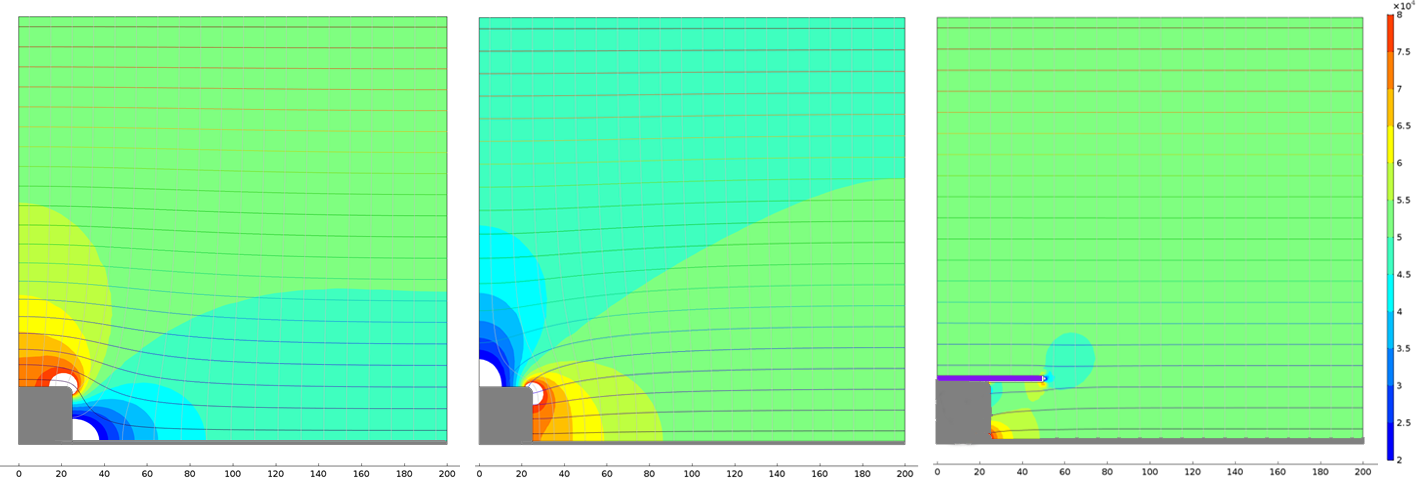
\includegraphics[width=0.95\textwidth]{field-shaping-strip-concept} %{ was Latest3D}
\end{dunefigure}

Other \dword{hv} components of the \dword{cpa} arrays include  edge aluminum profiles to act as the first elements of the \dword{fc} and cable segments forming the \dword{hv} bus.
%\fixme{'first elements' of the fc itself or, e.g., of fc modules, or of an fc endwall plane? (Anne) - In this case fc itself is correct. Left wording  RKP}

Figure~\ref{fig:cpa_panel-complete} pictures a completed \dword{pdsp} \dword{cpa} panel on the production table ready for lifting into vertical position. % for mounting on its trolley.

\begin{dunefigure}[Completed \dword{pdsp} \dword{cpa} panel on production table]{fig:cpa_panel-complete}{Completed \dword{pdsp} \dword{cpa} panel on production table.}
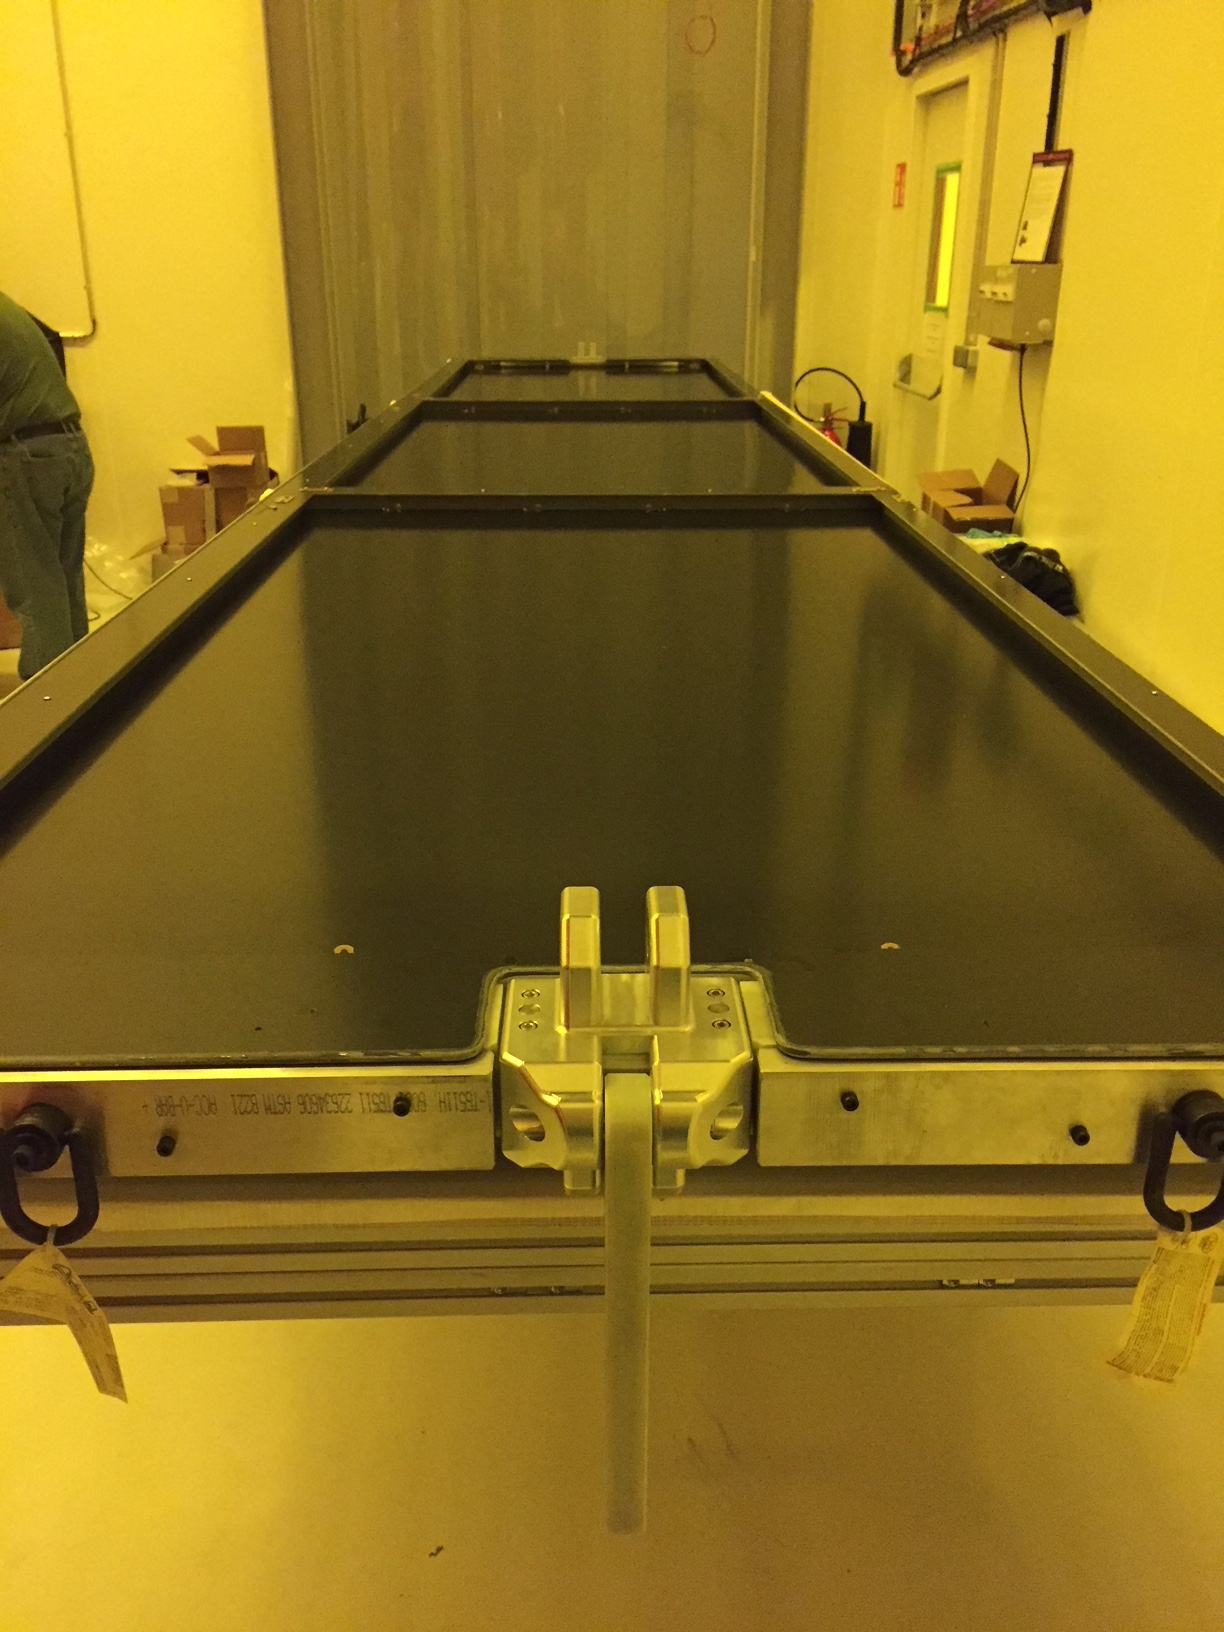
\includegraphics[width=0.5\textwidth]{cpa_panel-complete}
\end{dunefigure}

All electrical connections on the \dword{cpa} array and between the \dword{cpa} array and other \dword{hv} system components (top, bottom, and \dwords{ewfc}) are redundant by at least a factor of two.  Connections between \dwords{rp} in a \dword{cpa} unit are four-fold redundant.  The \dword{hv} connection from the \dword{hv} power supply is a closed loop around the \dword{cpa} that can sustain at least one broken connection without loss of the cathode \dword{hv}.  This ensures compliance with requirement SP-HV-2.
%\fixme{deleted plane here after cathode since it was not the defined Plane - SRM}

%\fixme{Idea: move next bit to an assembly or qc section?}
Careful inspection of these items during the assembly process ensures that no sharp points or edges are present. The surface resistivity of the \dword{cpa} \dwords{rp} and the \dword{fss} are checked multiple times during assembly -- first when the resistive panels and strips are received and after assembly into \dword{cpa} units on the table.  Coated parts that do not meet the minimum surface resistivity requirement are replaced.  This ensures that requirement TOP-17 is satisfied. 



%%%%%%%%%%%%%%%%%%%%%%%%%%%%
\section{Field Cage}

%\subsubsection{Overview} %General Considerations}
%\label{sec:fdsp-hv-des-fc-ov}

%A uniform \efield{} is required to drift ionization electrons towards the \dwords{apa}. To define the required uniform field, the top, bottom and sides of each drift volume are covered by a \dfirst{fc}.  
The \dword{fc} is introduced in Section~\ref{sec:fdsp-hv-des-fc}. Its function, basic characteristics and components are described there. 

The \dword{fc} %have been 
is designed to %ensure they 
meet the system specifications listed in Section~\ref{sec:fdsp-hv-des-consid}. %Table~\ref{tab:hvphysicsreqs}. 
To allow the system to reach the design \efield{} uniformity 
(specification SP-FD-11), 
%(specification~\ref{tab:spec:hvs-field-uniformity}) %(requirement 1) 
all components other than the aluminum profiles, \dwords{gp}, and electronic divider boards are made of insulating FRP and \frfour materials, and the end of each profile is covered with a \dword{uhmwpe} end cap. \\


All voltage divider boards provide redundancy for establishing the profile-to-profile potential differences with only minor distortions to the \efield in case of failure of any individual part, and two redundant boards provide the connection from the \dwords{fc} modules to the \dword{cpa} 
(specification SP-HV-2).
%(specification~\ref{tab:spec:hv-connection-redundancy}). %(requirement 6).
\fixme{Reference to specs table did not work, hardcoded here.- RKP}
%\fixme{This paragraph duplicates some of the text in the FC profiles section  - BY}
The aluminum profiles are attached to fiber-reinforced plastic (FRP) pultruded structural elements, including I-beams and box beams.  
Pultruded FRP material is non-conductive and strong enough to withstand the \dword{fc} loads  in the temperature range of \SI{-150}{C} and \SI{23}{C}, as certified by vendors. Testing of the FRP joints were conducted at liquid nitrogen temperatures~\cite{bib:docdb1504}. 
The material was stronger at these temperatures than at room temperature, 
providing confidence in the material behavior at \lar  temperature. The FRP material meets class A standards for fire and smoke development established by the International Building Code characterized by ASTM E84.\footnote{\textit{Standard Test Method for Surface Burning Characteristics of Building Materials}, ASTM International, \url{https://compass.astm.org/EDIT/html_annot.cgi?E84+18}.}

%\fixme{RP to check: add citations in bib: CPA and FC Design, DUNE DocDB 1504. Anne:1504 already in bib; need others? RKP- no.}
The top and bottom \dwords{fc} %modules 
are supported by the \dword{cpa} and \dword{apa} arrays. The \dwords{ewfc} modules, 
\SI{1.5}{\m} tall by \SI{3.5}{\m} long, are stacked eight units high (\SI{12}{\m}), and are supported by the installation rails above the \dword{cpa} and \dword{apa} arrays.

%and \dword{ewfc}  modules to define a uniform drift field of \spmaxfield{}, with an increasing potential over \SI{3.5}{m} from the \dword{hv} \dword{cpa} (\SI{-180}{kV}) to ground potential at the \dword{apa} sensor planes.
%The \dword{fc} consists of modules of extruded field-shaping aluminum electrodes (profiles), as listed in Table~\ref{tab:fcparts}. %, biased at stepped potentials. %, forming a barrel surrounding the top, bottom, and ends of the active drift volumes. The electrodes are  to establish the uniform field. % inside the \dword{lar} volume.
%The \dword{spmod} uses extruded aluminum profiles as a cost-effective way to establish the equipotential surfaces. 

%%%%%%%%%%%%%%%
\subsection{Field Cage Profiles}
\label{sec:fdsp-hv-des-fc-profiles}

The \dword{fc} consists of modules of extruded field-shaping aluminum %electrodes (
profiles, as listed in Table~\ref{tab:fcparts}. The shape of these %electrodes 
profiles is critical as it determines the strength of the \efield{} between a given profile and its neighbors, and between a profile and 
other surrounding parts, including the ground plane.
%, which is electrically at ground. % level. 
%Electric fields need to be  below \SI{30}{\kilo\volt/\centi\meter} 
%to satisfy design specification~\ref{tab:spec:local-e-fields} %requirement (2) 
%and enable safe \dword{tpc} operation~\cite{Blatter:2014wua}. % [A. Blatter, et al., JINST 9 (2014) P04006] %(design requirement 2).

The commercially available profiles used for both \dword{pdsp} and the \dword{spmod} design are estimated to lead to \efield{}s of up to \SI{12}{\kilo\volt\per\centi\meter} under the 
configuration and operating voltage assumptions.
Figure~\ref{fig:profile-e-field} illustrates results from an \efield{} calculation.

\begin{dunefigure}
[\efield map and equipotential contours of profiles at \SI{-180}{\kV}]{fig:profile-e-field}
{\efield map (color) and equipotential contours of an array of roll formed profiles biased up to \SI{-180}{\kV} and a ground clearance of \SI{20}{\cm} (Credit: BNL CAD model).} 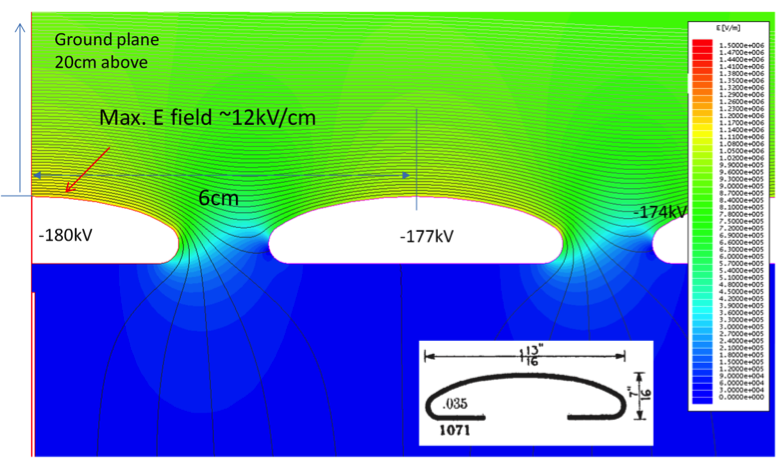
\includegraphics[width=0.8\textwidth]{profile-e-field.png}
\end{dunefigure}

The profile ends are equipped with \dword{uhmwpe} caps to reduce the risk of arcing.  These caps are designed %with sufficient wall thickness (\SI{6}{\milli\m}) 
to withstand the full voltage across their \SI{6}{\milli\m} thickness. 

The profiles have been carefully modeled to study the resulting \efield{}, 
and small-scale laboratory tests have %been conducted to 
ensured that the maximum \efield{} does not approach \SI{30}{\kV\per\cm}
~\cite{Blatter:2014wua}(specification SP-FD-24)
%(specification~\ref{tab:spec:local-e-fields}) %(requirement 2). 
%These design features are expected to avoid sparking
These features are designed to avoid sparking, and thus to draw very small stable currents, 
which should produce a consistent load on the power supply (specifications SP-FD-12, SP-FD-17, and SP-HV-1).
%(specifications~\ref{tab:spec:hv-ps-ripple}, \ref{tab:spec:cathode-resistivity}, and \ref{tab:spec:power-supply-stability}) %(requirements 3, 4, and 5). 
 %showed that the strength of the material increases at cryogenic temperature relative to room temperature, providing confidence in FRP material behavior at LAr temperature.
%FRP has all of the reinforcing fibers running along the main axis of the section being used. 

%A resistive divider chain interconnects %all 
%the aluminum profiles to provide a linear voltage gradient between the cathode and anode planes.  The top and bottom modules are nominally \SI{2.3}{\m} wide by \SI{3.5}{\m} long. 

%\fixme{Safety info}


%%%%%%%%%%%%%%%
\subsection{Ground Planes}
\label{sec:fdsp-hv-des-fc-gp}

For safe and stable operation of the \lar cryogenics system, the cryostat requires a small fraction of its volume to be filled with gaseous argon. This small volume is commonly referred to as the ullage. To optimize use of the \lar in the cryostat, we will place the upper \dword{fc}, which forms the top boundary of the \dword{tpc}, close to, but below, the liquid surface.

However, the ullage contains many grounded %metallic 
conducting components with sharp features, near which the \efield could easily exceed the breakdown strength of gaseous argon if directly exposed to the upper \dword{fc} below. To shield the high \efield from entering the gas ullage and prevent such breakdowns, % in the argon gas, 
\dfirsts{gp}, %is added above the upper \dword{fc} electrodes at a safe distance but still below the liquid surface.  
in the form of tiled, perforated stainless steel sheet panels, are mounted on the outside surface of the 
\dword{topfc} module with a \SI{30}{\cm} clearance.  This distance represents a 50\% increase over the value used in \dword{pdsp}, to further reduce the maximum E field in the TPC. 
The need for such shielding diminishes toward the \dword{apa} end of the \dword{fc} due to the lower voltages on the \dword{fc} profiles in that region. %Therefore the \dword{gp} on the top only covers about \SI{70}{\%} of the \dword{cpa} side of the \dword{fc}, leaving extra room for cable routing near the \dwords{apa}. \fixme{covers the highest voltage 70\% of the top, leaving the lowest part uncovered? }

In addition to the increase in FC to GP clearance, we are also eliminating most of the insulating standoffs supporting the GP tiles off the FC I-beams used in \dword{protodune}, in particular, those near the CPA end of the FC.  These standoffs  are deemed at risk of aiding discharges by providing a short path from FC to GP along corresponding straight edges.  Figure~\ref{fig:new-fc} pictures the new configuration. Figure~\ref{fig:new-fc_mockup} illustrates a test stand realized to demonstrate the coupling between FC and GP, with the standoffs near the cathode end removed. 

\begin{dunefigure}
[current baseline FC+GP module design]
{fig:new-fc}
{A side and a 3D views of the current design of the connection between FC and GP, with the standoffs near the cathode end removed. (Credit: ANL CAD model).}%
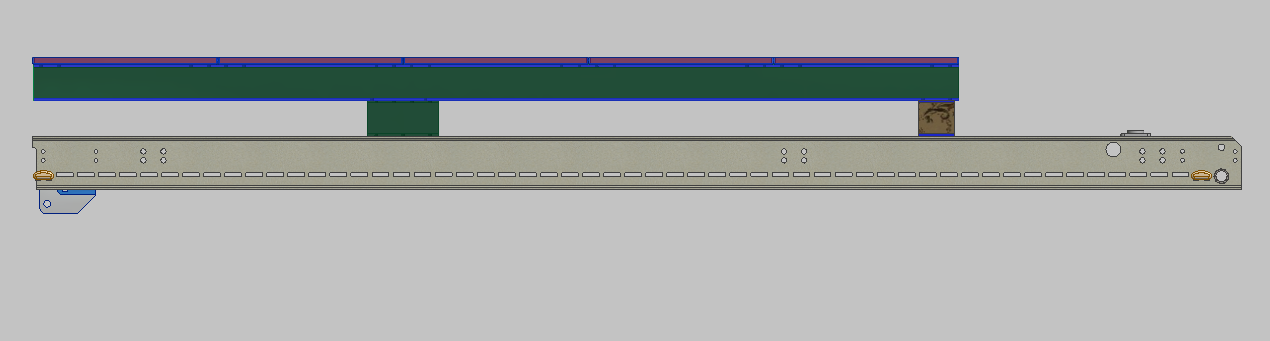
\includegraphics[width=0.8\textwidth]{fc_gp_baseline_side_view.png}
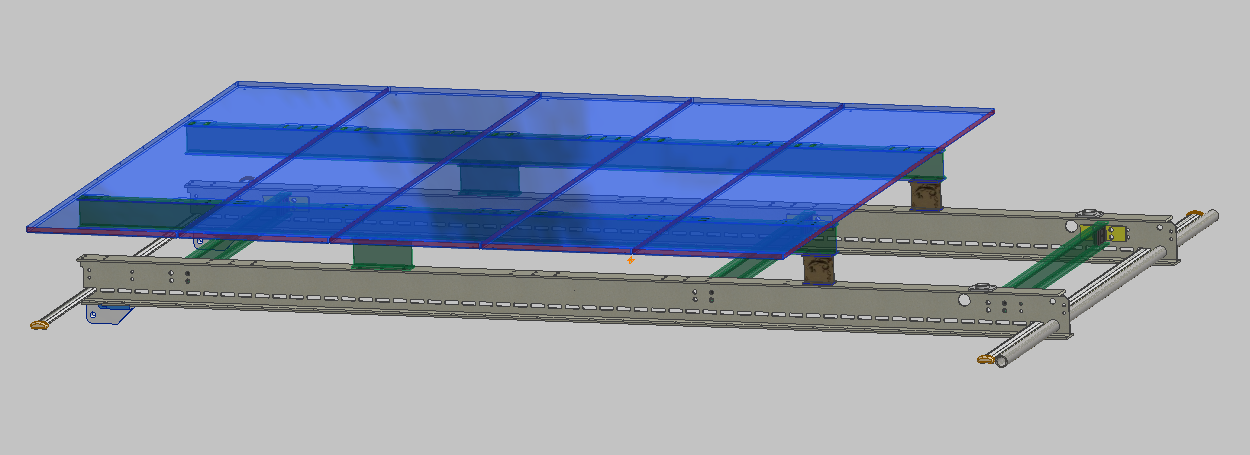
\includegraphics[width=0.8\textwidth]{fc_gp_baseline_3d_view.png}
\end{dunefigure}

\begin{dunefigure}
[current baseline FC+GP module design]
{fig:new-fc_mockup}
{Pictures of a test module of demonstrating the coupling between FC and GP, with the standoffs near the cathode end removed. (Credit: Univ. of Minnesota).}%
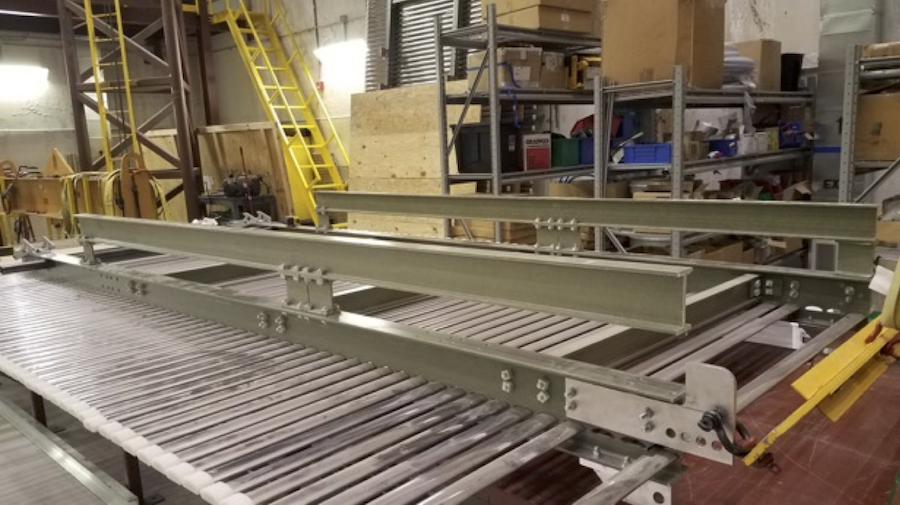
\includegraphics[width=0.48\textwidth]{FC_mockup-1.png}
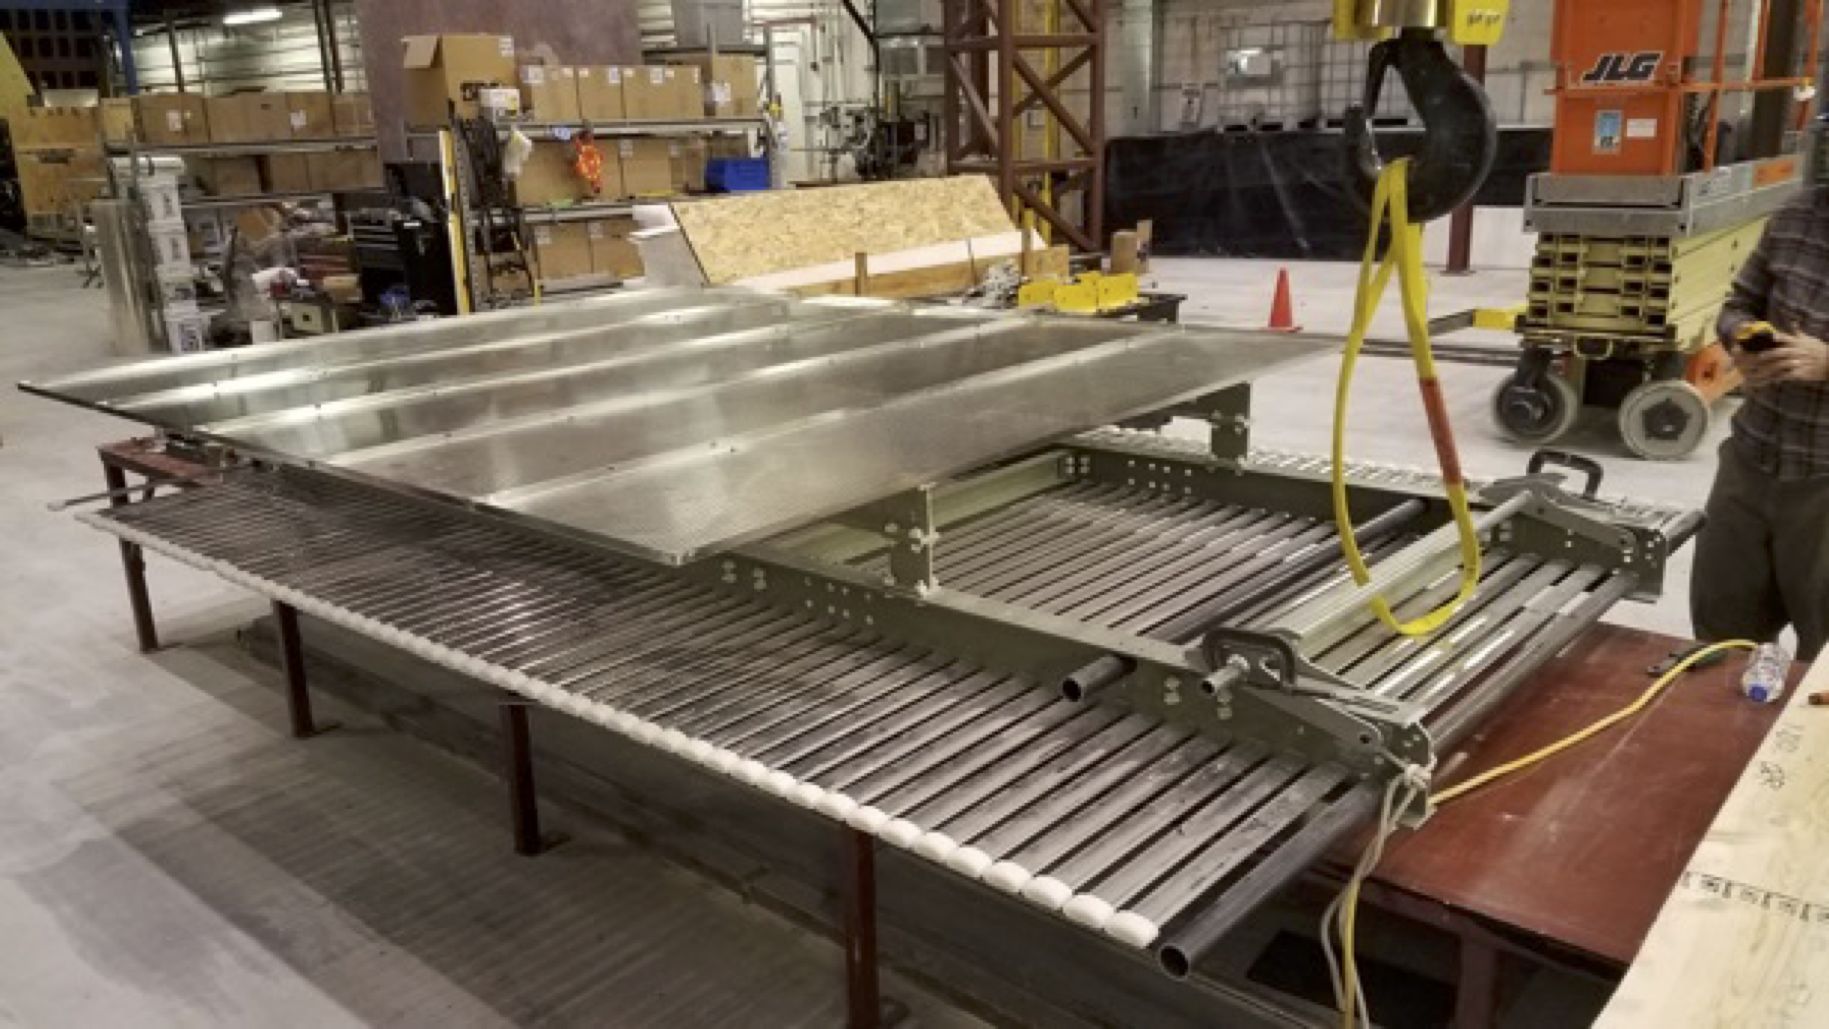
\includegraphics[width=0.48\textwidth]{FC_mockup-2.png}
\end{dunefigure}

On the bottom of the cryostat a similar set of \dwords{gp} %is planned to 
will protect against %prevent 
breakdown in the liquid near cryogenic pipings and other sensors with sharp features. The same clearance will be used. No \dwords{gp} are planned beyond the two \dwords{ewfc} since there is sufficient clearance in those regions.  
%\fixme{end GP section}

%As discussed in Section~\ref{sec:fdsp-hv-intro}, the field cage modules are of two types: the similar top and bottom \dword{fc} and the \dword{ewfc}, both of which are described below. 

%A resistive divider chain interconnects all the aluminum profiles to provide a linear voltage gradient between the cathode and anode planes.  The top and bottom modules are nominally \SI{2.3}{\m} wide by \SI{3.5}{\m} long. A \dword{gp}, in the form of tiled, perforated stainless steel sheet panels, is mounted on the outside surface of the T/B field cage module with a \SI{20}{\cm} clearance. The top and bottom \dword{fc} modules are supported by the \dwords{cpa} and \dwords{apa}. The \dword{ewfc} modules are \SI{1.5}{\m} tall by \SI{3.5}{\m} long. They are stacked eight units high (\SI{12}{\m}), and are supported by the installation rails above the \dwords{apa} and \dwords{cpa}.

%%%%%%%%%%%%%%%
\subsection{Maximum Field Distortions}

The \dwords{fc} are designed to produce a uniform \efield with understood characteristics.
%The %current (i.e., \dword{pdsp}) 
%\dword{fc} design has a large gap between the endwall module and its neighboring top and bottom modules to allow the latter two to swing past the \dword{ewfc} during \dword{fc} deployment. This gap causes the largest known \efield distortion in the \dword{tpc}. Figure~\ref{fig:fc-distortion} shows the extent of the distortion in this limiting scenario. In \dword{pdsp}, the gap produces two regions (of total \lar mass \SI{20}{kg}) in the TPC near both bottom corners that suffer \SI{5}{\%} \efield distortions.
The largest known \efield distortion in the \dword{tpc} occurs around a large gap in the \dword{fc} between the endwall module and its neighboring top and bottom modules. This gap is necessary to allow the top and bottom to swing past the \dword{ewfc} during deployment.  Figure~\ref{fig:fc-distortion} illustrates the extent of the distortion in this limiting scenario. 
If this feature remains in the \dword{spmod}, a total \lar mass of \SI{160}{kg} along these 4 edges of the TPC suffers $>$\SI{5}{\%} \efield distortions.

\begin{dunefigure}[\efield at edge of \dword{fc}]
{fig:fc-distortion}
{\efield at a corner between the bottom and endwall \dword{fc} modules, showing effects of a \SI{7}{cm} gap. Left: the extent of \num{5}\% \efield{} non-uniformity boundary (black surface, contains less than \SI{10}{kg} of \lar) and \num{10}\% non-uniformity boundary (white surface, contains $\sim$ \SI{6}{kg} of \lar) inside the TPC's active volume. The inset is a view from the CAD model.  Right: electron drift lines originating from the cathode surface.}
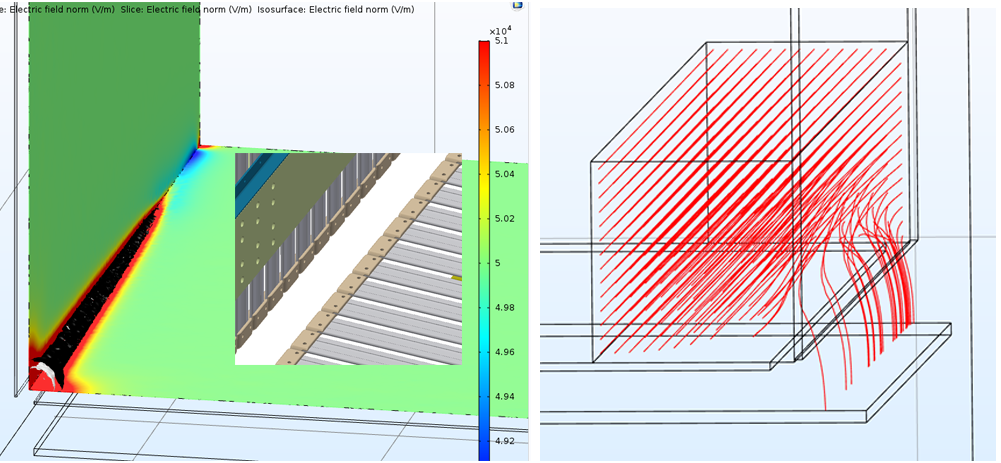
\includegraphics[width=0.9\textwidth]{distortion_from_fc_gap}
\end{dunefigure}



%%%%%%%%%%%%%%%%%%%%%%%%%%%
\subsection{Top and Bottom Field Cage Modules}

The \dword{topfc} and \dword{botfc} module dimensions are listed in Table~\ref{tab:fcparts}. The length, \spfcmodlen{}, is set by the length of the two \SI{15.2}{\cm} (\SI{6}\,in) FRP I-beams that form the primary support structure of the modules. The I-beams are connected to each other by three  \SI{7.6}{\cm} (\SI{3}\,in) FRP cross beams. The connections between the longitudinal and cross I-beams are made with L-shaped FRP braces that are attached to the I-beams with FRP spacer tubes, and secured with FRP threaded rods, FRP hex-head nuts, and custom-machined \frfour washer plates.

The \SI{2.3}{\m} module width corresponds to the length of the aluminum profiles, including the UHMW polyethylene end caps. Profiles are secured to the FRP frame using custom-machined double-holed stainless steel slip nuts that are slid into and electrically in direct contact with the aluminum profiles such that they straddle the webbing of the \SI{15}{\cm} I-beams, and are held in place with screws that penetrate the I-beam flanges. The profile offset with respect to the FRP frame is different for modules closest to the \dwords{ewfc}, %endwalls, 
and modules in the center of the active volume.

Five \dwords{gp} are connected to the outside (i.e., the non-drift side) of each \dword{topfc} and \dword{botfc} module. The \dwords{gp} are positioned $\sim$\SI{30}{\cm} away from the profiles, and begin at the \dword{cpa} end of the module, leaving the last 14 profiles (\SI{88}{\cm}) on the \dword{apa} end of the module exposed. Between the \dwords{gp} and the \SI{15}{\cm} I-beams, standoffs made of short sections of \SI{10.2}{\cm} (4\,in)  FRP I-beams are connected with FRP threaded rods and slip nuts. The electrical connection between the \dwords{gp} is made with copper strips.

The connections between the top and bottom modules and the \dwords{cpa} are made with aluminum hinges, \SI{2.54}{\cm} (1\,in) in thickness, that allow the modules to be folded in on the \dword{cpa} during installation. The hinges are electrically connected to the second profile from the \dword{cpa}. The connections to the \dwords{apa} are made with stainless steel latches that are engaged once the top and bottom \dword{fc} modules are unfolded and fully extended toward the \dword{apa}.

The voltage drop between adjacent profiles is established by voltage divider boards screwed into the drift-volume side of the profiles. A custom-machined nut plate %is used that can be 
is inserted into the open slot of each profile and twisted \SI{90}{\degree} %$^\circ$ 
to lock into position. Two additional boards to connect the modules to the \dwords{cpa} %were screwed 
screw into the last profile on the \dword{cpa} end of the module. This system is %also 
more fully described in Section~\ref{sec:fdsp-hv-design-interconnect}. A fully assembled module is pictured in Figure~\ref{fig:tbfc1-2}.

\begin{dunefigure}[Top and bottom field cage modules]{fig:tbfc1-2}{A fully assembled module with ground planes is shown.} %as well as a closeup of a \dword{cpa} end as viewed from the bottom (drift) side of the module.}
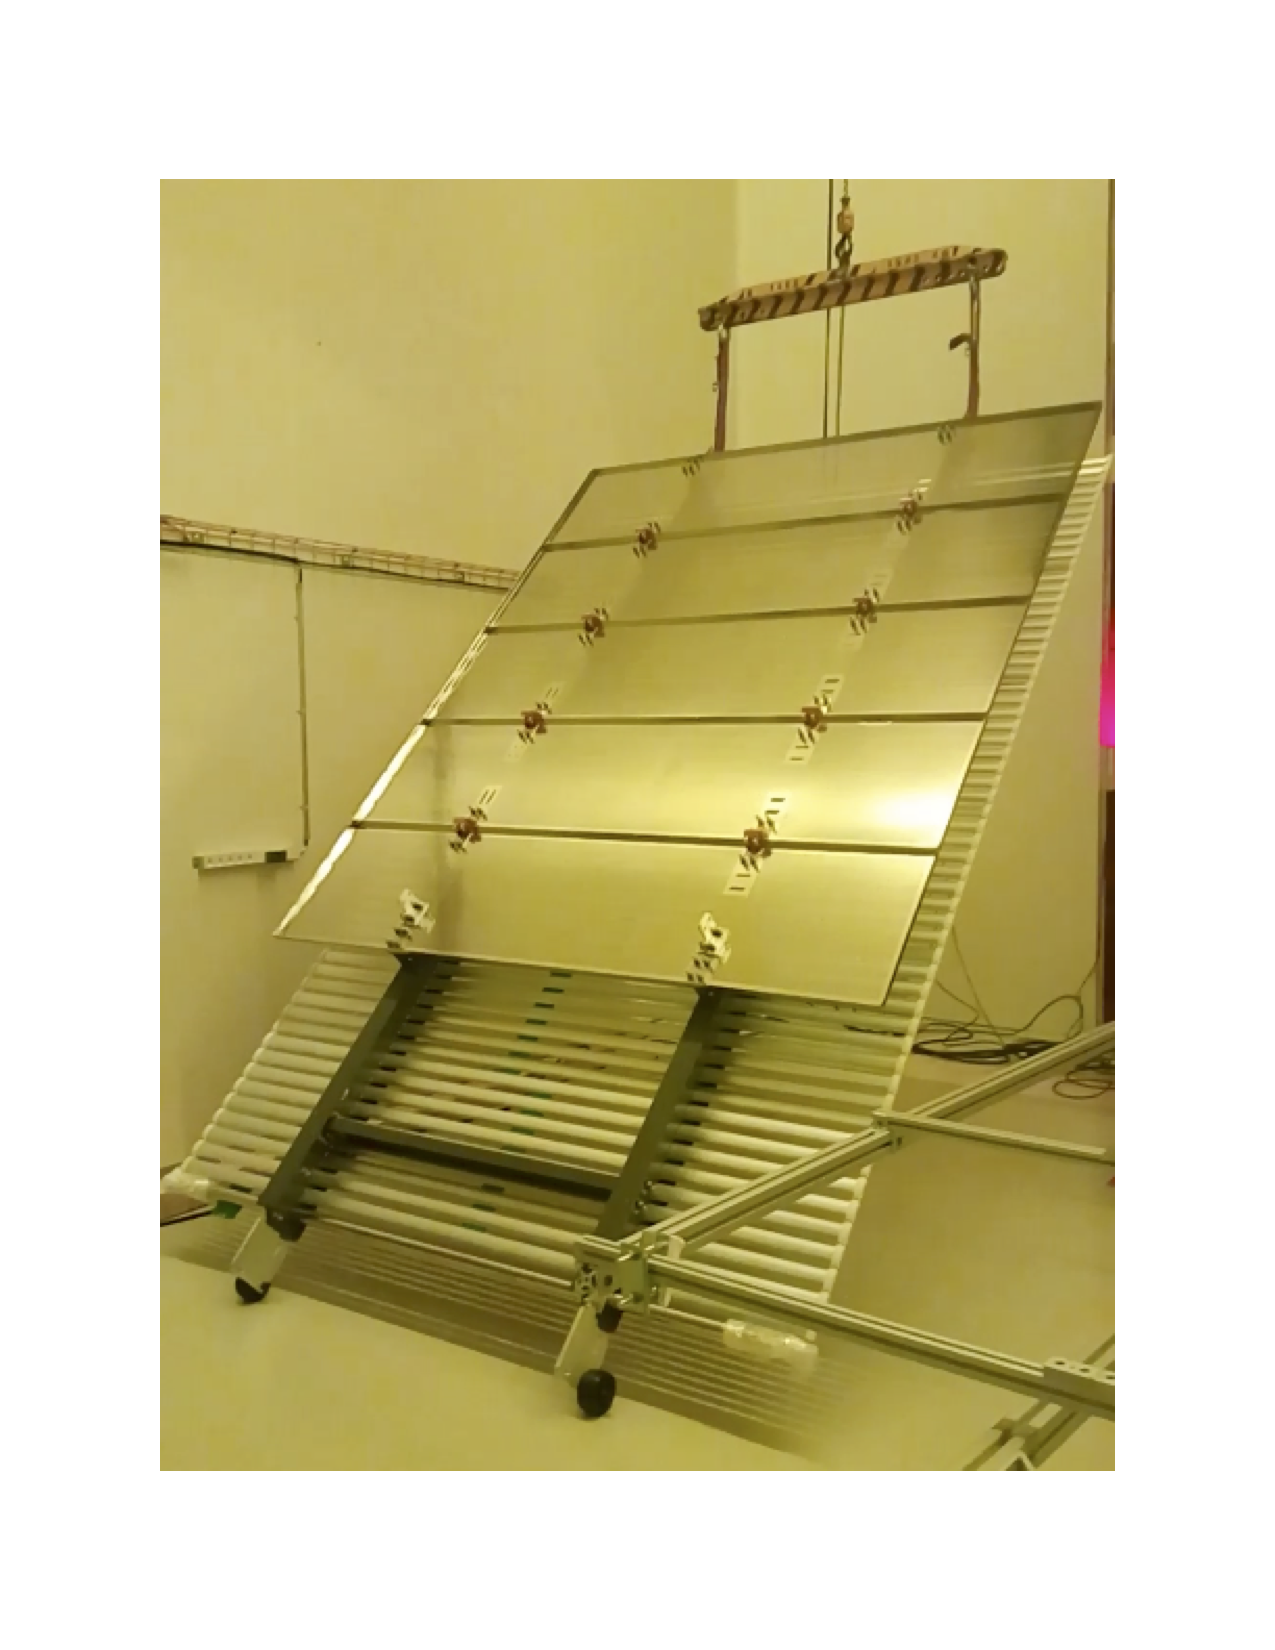
\includegraphics[width=0.45\textwidth]{FC_with_GP}
%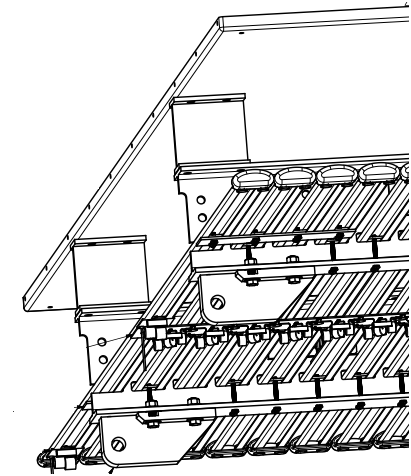
\includegraphics[width=0.33\textwidth]{tbfc2}
\end{dunefigure}
%\fixme{Caption needs improvement, and labels would be useful on diagrams. Anne}


\subsection{Endwall field cages (EWFC)}

%The endwall field cage (\dword{ewfc}) for each of the four drift volumes consists of two endwalls (EW), one on each side of the drift volume. Each endwall is in turn composed of eight endwall modules (EW-Modules). 

Each of the four drift volumes has two \dwords{ewfc}, one on each end. Each \dword{ewfc} is in turn composed of eight \dword{ewfc} modules.
There are two different types of \dword{ewfc} modules, each of which comes in a \textit{regular} and in a \textit{mirrored} configuration to account for 
mounting constraints and to match the detector geometry. Figure~\ref{fig:fc_endwall_panels} illustrates the layout for the topmost 
and the other panels, respectively.

\begin{dunefigure}[Endwall \dword{fc} panels]{fig:fc_endwall_panels}{Left: Uppermost panel of the \dword{ewfc}. Right: Non-uppermost \dword{ewfc} panel.}
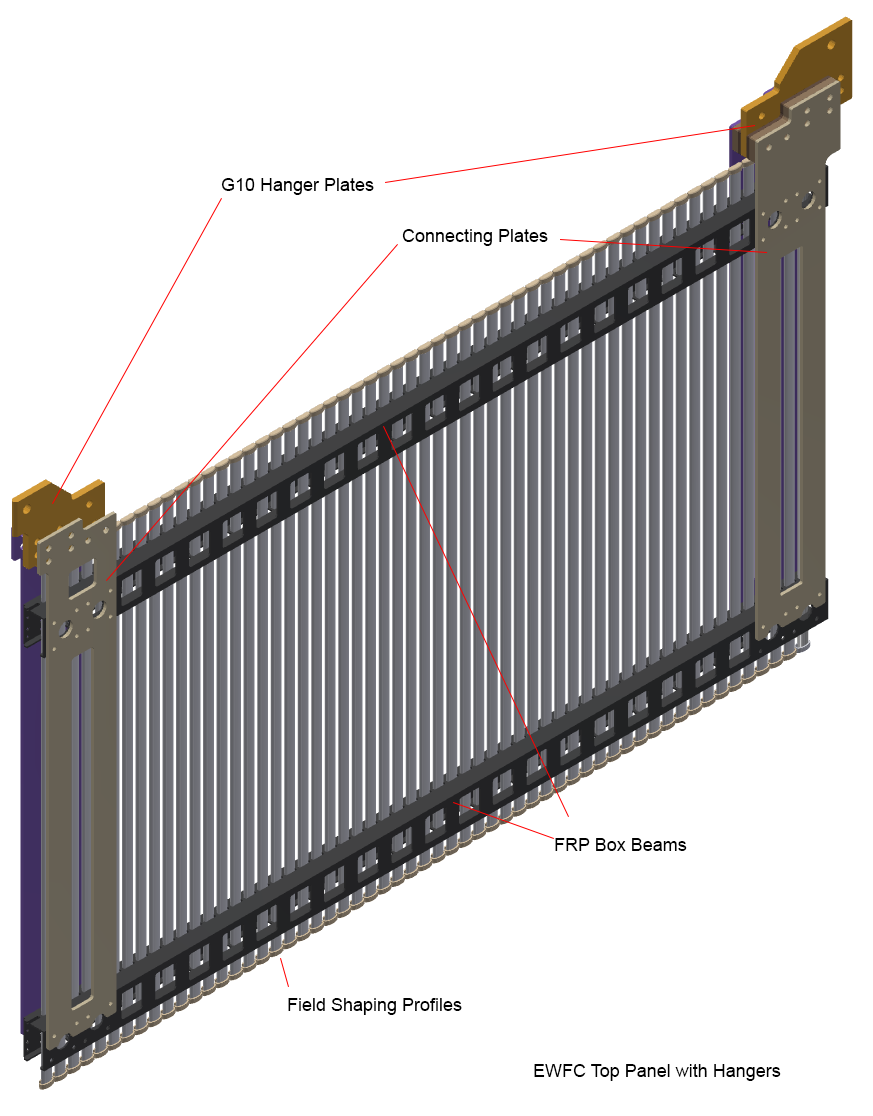
\includegraphics[width=0.48\textwidth]
{EWFC_Top_Module}
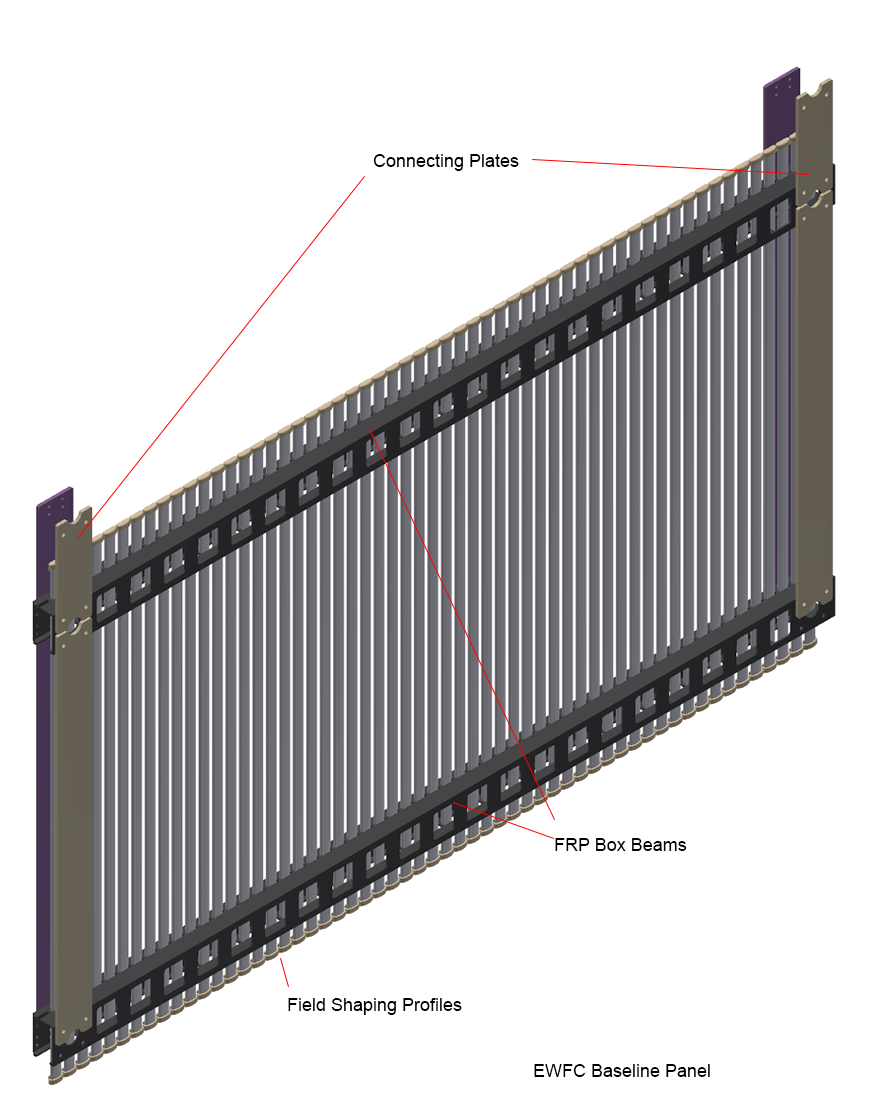
\includegraphics[width=0.48\textwidth]
{EWFC_Baseline_Module}
\end{dunefigure}

Each \dword{ewfc} module is constructed of two FRP box beams, each \SI{3.5}{\m} long, as shown in \ref{fig:fc_endwall_panels}. 
The box beam design also incorporates cutouts on the outside face to minimize charge build up. Box beams are connected using \SI{1.27}{\cm} (\num{0.5}\,in) thick FRP plates. The plates are connected to the box beams using a shear pin and bolt arrangement. The inside plates facing the active volume are connected using special stainless steel slip nuts and stainless steel bolts. The field-shaping profiles are connected to the top box beam using stainless steel slip nuts, an FRP angle, and two screws each that pass through matching holes in the wings of the aluminum profiles. At the bottom box beam the profiles are pulled against another FRP angle with a single screw and a slip nut that is held in place by friction.

%\begin{center}
%   \parbox[t]{0.47\textwidth}{
 %  \resizebox{0.47\textwidth}{!}{\includegraphics[width=0.48\textwidth]{\dword{fc}endwall_top-panel.png}}
%\caption{\label{fig:\dword{fc}endwall_top} Uppermost panel of the field cage endwall. {\color{red} NOTE: need to replace figure with updated version for DUNE, e.g. without middle FRP cross member.}}}
%\makebox[0.025\textwidth]{}
 %  \parbox[t]{0.48\textwidth}{
 %  \resizebox{.48\textwidth}{!}{\includegraphics[width=0.48\textwidth]{\dword{fc}endwall_panel.png}}
%\caption{\label{fig:\dword{fc}endwall_panel} Baseline field cage panel. {\color{red}NOTE: need to replace figure with updated version for DUNE, e.g. without middle FRP cross member.}}}
%\end{center}

\subsection{Voltage divider boards}
A resistive divider chain interconnects all the metal profiles of each FC modules to provide a linear voltage gradient between the cathode and anode planes.

The resistive divider chain is realized with Resistor Divider Board hosting eight resistive stages in series. Each stage (corresponding to \SI{6}{cm} gap between FC profiles)  consists of two \SI{5}{\giga\ohm} resistors in parallel yielding a parallel resistance of \SI{2500}{\mega\ohm} per stage to hold a nominal voltage difference of \SI{3}{kV}. Each stage is protected against high voltage discharge transients by transient/surge absorbers (varistors). To achieve the desired clamping voltage, three varistors (with \SI{1.8}{kV} clamping voltage) are wired in series and placed in parallel with the associated resistors. A schematic of the Resistor Divider Board is shown in Figure~\ref{fig:ResDivBoa}; an illustration of the Resistor Divider Board used in \dword{pdsp} is shown as well.

\begin{dunefigure}[\dword{hv} Resistor Divider Board]{fig:ResDivBoa}
  {Left: A \dword{pdsp} Resistor Divider Board. Right: Schematic diagram of Resistor Divider Board}
  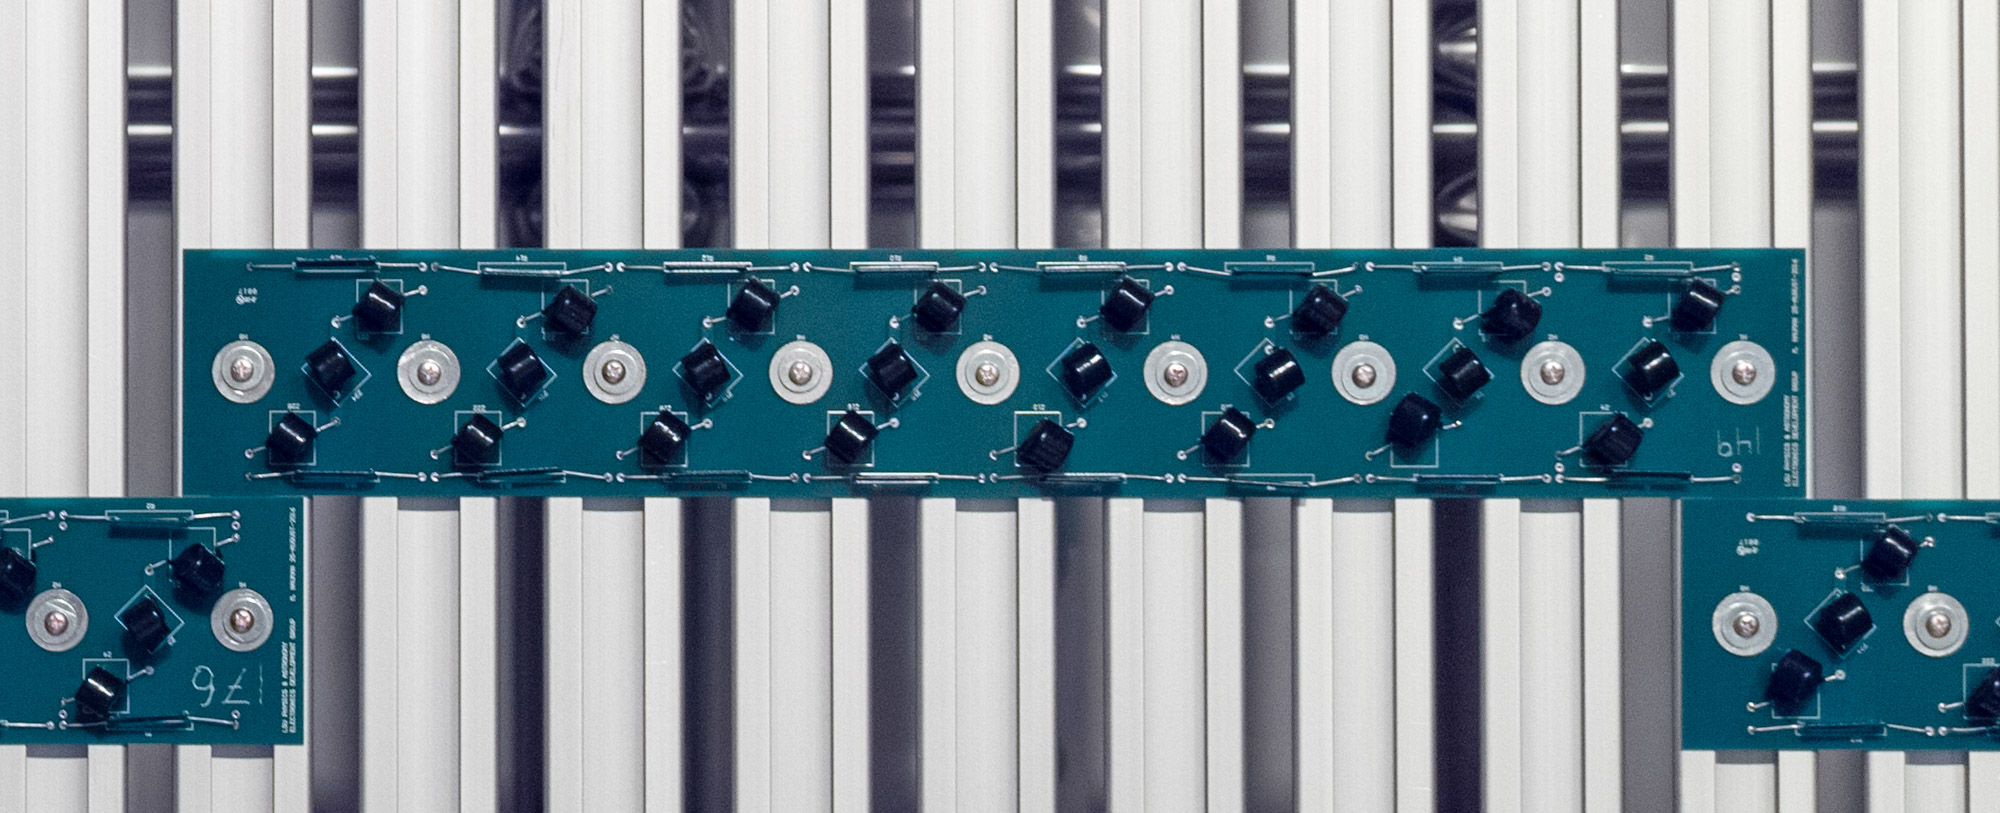
\includegraphics[width=0.48\textwidth]{Divider_board.jpg}
  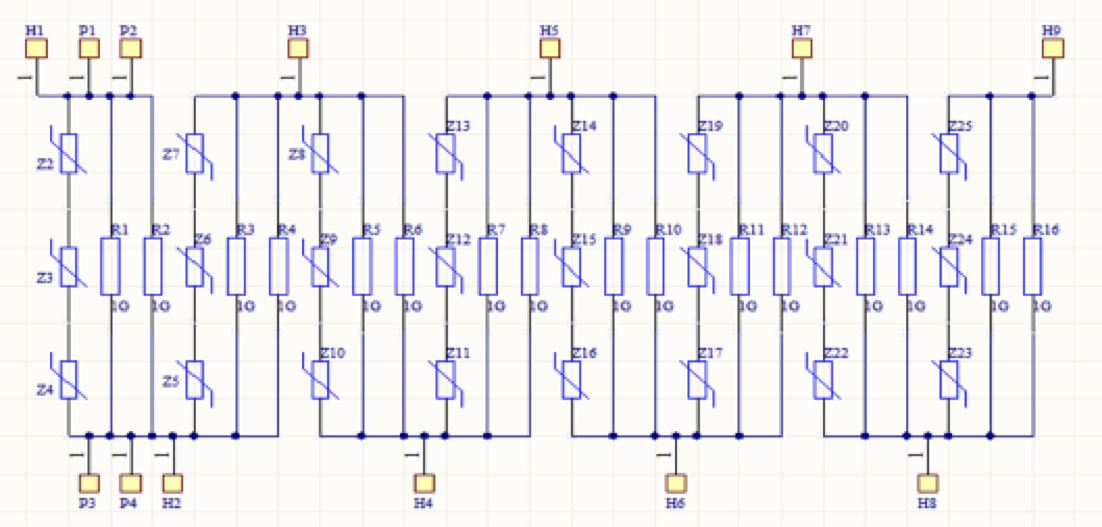
\includegraphics[width=0.48\textwidth]{ResDivBoa.png}
\end{dunefigure}

These boards will be identical to the ones successfully mounted in ProtoDUNE-SP field cage. 

The current drawn by each divider chain is about $1.2~\mu A$ at the nominal Electric Field of $500~V/cm$. A total of 132 resistive divider chain are connected in parallel to each CPA array for a total of about $158~\mu A$, well within the capability of the selected HV power supply.

There are about 30,000 resistors used on the FCs in a \dword{spmod}. A resistor failure is a possible risk to the TPC.  
An open resistor, the most common failure mode, on the divider chain would approximately double the voltage across the remaining resistor to \SI{6}{kV}.  This larger voltage would force the three varistors in parallel to that resistor into conduction mode, resulting in a voltage drop of roughly \SI{5}{kV} (\SI{1.7}{kV} $\times$ \num{3}), while the rest of the divider chain remains linear, with a slightly lower voltage gradient. 
Because the damage to the divider would be local to one module, its impact to the \dword{tpc} drift field is limited to region near this module, a benefit of the modular FC design.
An example of a simulated \efield{} distortion which would be caused by a failed resistor is shown in Figure~\ref{fig:fc-broken-resistor}. 

\begin{dunefigure}[\efield distortion from broken voltage divider path]{fig:fc-broken-resistor}{Simulated \efield{} distortion from one broken resistor in the middle of the voltage divider chain on one bottom field cage module, emphasizing the need for redundancy. Left: Extent of \efield{} non-uniformity in the active volume of the TPC. the green planes mark the boundaries of the active volume inside the field cage. The partial contour surfaces represent the volume boundaries where \efield{} exceeds 5\% (dark red, contains less than 100\,kg of LAr) and 10\% (dark blue, contains less than 20\,kg of LAr) of the nominal drift field. The units are \si{\volt\per\m} in the legend. Right: electron drift lines connecting the \dword{cpa} to \dword{apa} in a bottom/end wall field cage corner.  The maximum distortion to the field line is about 5\,cm for electrons starting at mid drift at the bottom edge of the active volume.}
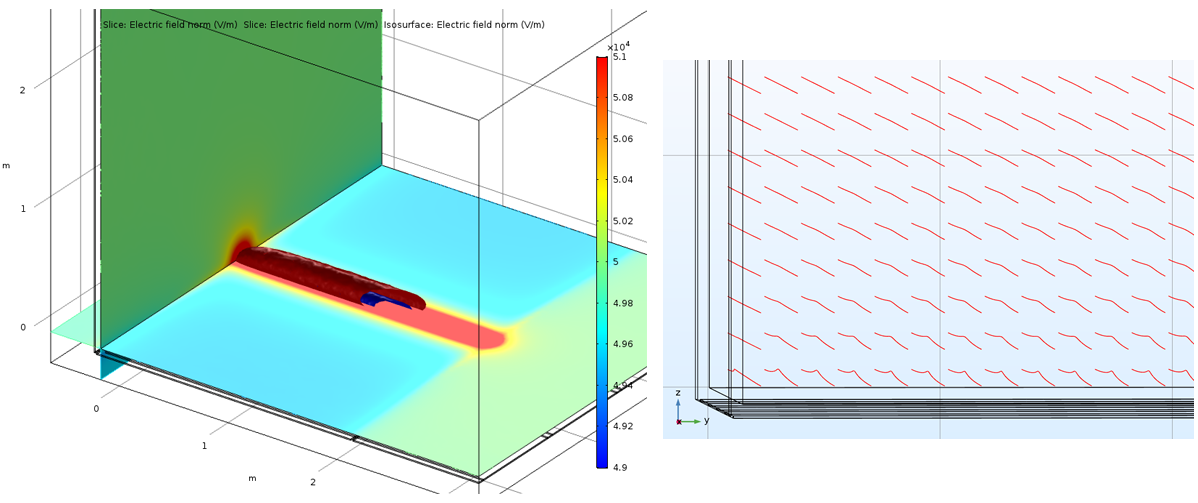
\includegraphics[width=0.9\textwidth]{e-field-distortion-due-to-open-resistor}
\end{dunefigure}
The effect of the non-uniformity in resistor values can also be scaled from this study.  A 2\% change in a resistor value (1\% change from the 2R in parallel) would give about 1.5\% of the distortion from a broken resistor, i.e. less than 1\,mm of transverse distortion in track position, with no noticeable drift field amplitude change inside the active volume.
 


%%%%%%%%%%%%%%%%%%%%%%%%%%%%
\section{Electrical Interconnections} % (Glenn)
\label{sec:fdsp-hv-design-interconnect}

\begin{dunefigure}[\dword{hv} interconnection topology]{fig:fdsp-hv-design-interconnect-concept}
  {High-level topology of the \dword{hv} interconnections}
  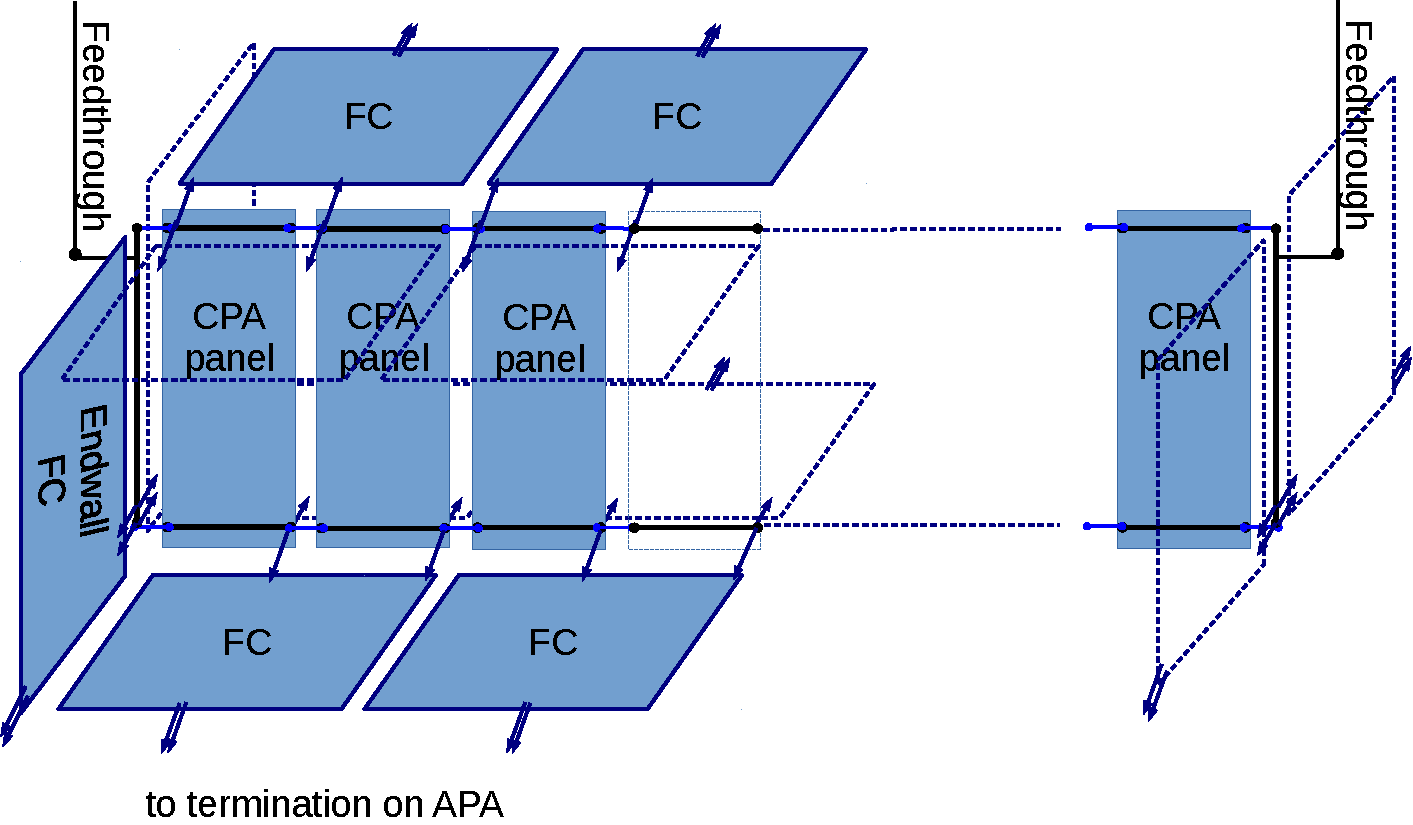
\includegraphics[width=0.7\textwidth]{fdsp-hv-interconnection-topology}
\end{dunefigure}
%\fixme{Figure \ref{fig:fdsp-hv-design-interconnect-concept} shows single-CPA-panel height as for \dword{pdsp} but implies 25 panels wide as for the FD module.  Anne }
%\fixme{This figure looks OK - the height of a CPA Panel at DUNE is 12 m - the CPA Panels drawn here are meant to be 12 m high and there are 50 of them in a 25 CPA Plane CPA Array - the electrical connections are made on CPA Panels, so in this drawing, the separate CPA Panels are shown - SRM}
Electrical interconnections are needed among the \dword{hv} delivery system, \dword{cpa} panels, \dword{fc} modules, and termination
boards on the \dword{apa} modules, as well as between resistive dividers and
the field-forming elements on the \dwords{cpa} and \dwords{fc}.  %\fixme{Assuming the 'field-forming elements' don't have other specific names, element is ok here. Anne RKP-refers to more than one kind of thing.}
Redundancy is
needed to avoid single points of failure. 
Some connections must be
insulated in order to avoid creating a discharge path that might
circumvent the discharge mitigation provided by the resistive \dword{cpa}
surface and \dword{fc} partitioning.  Certain connections must be
flexible in order to allow for \dword{fc} deployment, thermal
contraction, and motion between separately supported \dwords{cpa} components.  Figure~\ref{fig:fdsp-hv-design-interconnect-concept} shows a high-level
overview of the interconnections between the \dword{hv}, \dword{cpa}, and \dword{fc} modules.


%% connections between major elements (\dword{hv}, \dword{cpa}, \dword{fc}, \dword{apa})
High voltage feedthroughs connect to cups mounted on the \dword{cpa} frame
%\cite the \dword{hv} delivery section
that attach to a \dword{hv} bus running through the \dwords{cpa}.  \Dword{hv} bus connections
between \dword{cpa} panels are made by flexible wires through holes in the
\dword{cpa} frame. The \dword{hv} bus is a loop in order to mitigate risk of a single
point failure; feedthroughs at each end of each \dword{cpa} panel mitigate
risk of a double-break failure.  Voltage dividers on each \dword{cpa} panel
bias the \dwords{fss} and the resistive dividers on the top
and bottom \dwords{fc}.  The \dword{cpa}-to-\dword{fc} connections are made using
flexible wire to accommodate \dword{fc} deployment.  To further
increase redundancy, two \dword{cpa} panels connect to each top or bottom
field cage, and two connections are also made to each \dword{ewfc}. Resistor divider boards attach directly to the interior side of
the \dword{fc} profiles with screws.   A redundant pair of flexible wires
connects a circuit board on the last profile of each \dword{fc} to a
bias-and-monitoring board mounted on the corresponding \dword{apa}.

%% connections within \dword{cpa}
Short sections of flexible wire at the ends of each \dword{hv} bus segment
attach to screws in brass tabs on the \dword{cpa} resistive panels (\dword{cpa} \dwords{rp}).
%\cite \dword{cpa} design subsection
Vertical \dword{hv} bus segments on the outer ends of each \dword{cpa} plane connect
the top and bottom \dword{hv} buses to complete the loop.  Solid wire is used
to connect resistive panels within a \dword{cpa} panel.

%% \dword{fc} connections
Each \dword{fc} module is as electrically independent as possible in order to
mitigate discharge.  However, only the bottom module of each endwall
can make connections to the \dword{hv} bus and \dword{apa}, so each endwall module
is connected to its upper neighbor at its first and last profiles
using metal strips.

%% added by BY
Each FC didvider chain connects to a FC termination board in parallel to a grounded failsafe circuit at the APA end.  The FC termination boards are mounted on the top of the upper APAs and bottom of lower APAs.  Each board provides a default termination resistance, and a SHV cable connection to the outside of the cryostat, via the CE signal feedthrough flange, through which we can either supply a different termination voltage to the FC, or monitor the current flowing through the divider chain.

%% Regarding wire terminals and screws
All flexible wires have ring or spade terminals and are secured by
screws in brass tabs.  Spring washers are used with every electrical
screw connection in order to maintain good electrical contact with
motion and changes of temperature.

Table \ref{tab:sp-hv-interconnects} summarizes the interconnections required 
for the HV system.

\begin{dunetable}
[\dword{hv} system interconnections]
{p{0.35\linewidth}p{0.62\linewidth}}
{tab:sp-hv-interconnects}
{\dword{hv} System Interconnections}   
 Connection & Method \\ \toprowrule
 \dword{hv} cup to \dword{hv} bus & wire to screw in \dword{hv} cup mount on \dword{cpa} frame \\ \colhline
 \dword{hv} bus between \dword{cpa} panels & wire between screws in brass tabs \\ \colhline
 \dword{hv} bus to \dword{fss} & wire to circuit board mounted on \dword{fss} \\ \colhline
 \dword{fss} to \dword{topfc} and \dword{botfc} & wire to circuit board on first \dword{fc} profile, two per \dword{fc} module \\ \colhline
 \dword{hv} bus to endwall \dword{fc} & wire to circuit board mounted on first \dword{fc} profile, two per endwall \\ \colhline
 \dword{fc} divider circuit boards & directly attached to profiles using screws and SS slip nuts \\ \colhline
 \dword{fc} to bias and monitoring termination & redundant wires from board mounted on last \dword{fc} profile \\ \colhline
 \dword{hv} bus to \dword{cpa} panels & brass tab on \dword{cpa} resistive panel \\ \colhline
 \dword{cpa} \dword{rp} interconnections & solid wire between screws in brass tabs \\ \colhline
 Endwall \dword{fc} module interconnections & metal strips, first and last profiles only
 \\ \colhline
\end{dunetable}

The redundancy in electrical connections described above meets requirement (6).
The \dword{hv} bus and interconnections are all made in low field regions in order to meet requirement (2).
The \dword{hv} bus cable is rated at the full cathode \dword{hv} such that even in case of a rapid discharge of the \dword{hv} system no current can flow to the cathode or \dword{fc} except at the intended contact points, preserving the ability of the resistive cathode and \dwords{fc} to meet requirement (5).


%%%%%%%%%%%%%%%%%%%%%%%%%%%%%%%%%%%%%%%%%%%%%%%%%%%%%%%%%%%%%%%%%%%%
\section{ProtoDUNE-SP High Voltage Experience}
%NOTE -- this is a work in progress... still needs to be refined...
%NOTE a nice number to quote somewhere in this section will be the uptime % during the beam run
\label{sec:fdsp-hv-protodune}

%\fixme{Can we avoid the term 'CPA plane' and just use 'panel'? That's what I'm trying to do earlier in chapter to avoid unnecessary confusion.  The language is different from the PDUNE TDR, too, which uses 'column'. Anne}
%\fixme{We defined each component of the CPA in the table at the beginning of the HV section for DUNE - A CPA Plane is distinct from a CPA Panel as defined in the table - if we use the defined definitions, there is no confusion.  We need a definition of the paired CPA Panels which we defined as a CPA Plane which is the unit of installation. This section is about ProtoDUNE which has slightly different definitions due to the difference in size, so in this section the components are described in lower case, i.e., array and panel and have their definitions in the text - SRM}

%From PDUNE SP TDR:  The cathode plane design chosen for the ProtoDUNE-SP TPC is an array of 18 moderately sized modules constructed from strong 6-cm-thick FR4 (the fire-retardant version of G10) frames. The frames hold 3-mm-thick FR4 panels laminated on both sides with a commercial resistive Kapton film. Each CPA module is 1.16m wide and 2m high, and they stack to form six CPA columns of height 6 m. The six-column-wide CPA has the same dimensions as each of the two APA planes,with a width of about 7 m.

\dword{pdsp} \cite{Abi:2017aow} is a prototype for a \dword{spmod}. %the single phase \lartpc \dword{dune} far detector.
Approximately one twentieth the size of a \dword{spmod}, this detector implements an A-C-A configuration with one \dword{cpa} array that bisects the TPC and two \dword{apa} arrays, one along each side. 
The \dword{cpa} array consists of %three full-size \dword{cpa} planes with dimensions \SI{2.3}{m} $\times$ \SI{6.0}{m} 
six \dword{cpa} panels, each \SI{1.2}{m} wide by \SI{6.0}{m} high (half-height relative to a \dword{spmod}), 
and is positioned \SI{359}{cm} away from each \dword{apa} array, matching the maximum drift distance of a \dword{spmod}.
%\fixme{In defs, we have max drift distance as \spmaxdrift. Can we replace 360cm?  RP to check}
%\fixme{This is protoDUNE so number is different. Replaced with 359 cm but still checking. NOTE - Defs file of 353 may actually be 352 cm, this could affect others}

Six top and six bottom \dword{fc} modules connect the horizontal edges of the \dword{cpa} and \dword{apa} arrays, and four %endwalls 
\dwords{ewfc} connect the vertical edges (two per drift volume).
Each \dword{ewfc} comprises of four endwall modules (half-height relative to a \dword{spmod}).
A Heinzinger $-$\SI{300}{kV} \SI{0.5}{mA} HV power supply delivers voltage to the cathode.
Two HV filters in series between the power supply and HV feedthrough filter out high-frequency fluctuations upstream of the cathode.

\begin{dunefigure}[ProtoDUNE-SP TPC HV components]
{fig:protodune_sp_hv}
{One of the two drift volumes of \dword{pdsp}. The \dword{fc} modules shown enclose the drift volume between the \dword{cpa} array (at the center of the image) and the \dword{apa} array (upper right). The \dwords{ewfc} are oriented vertically; the top and bottom units are horizontal. The staggered printed circuit boards connecting the \dword{ewfc} profiles are the voltage divider boards. %which introduce a uniform resistance between neighboring electrodes. (this part is in regular text Anne)
}
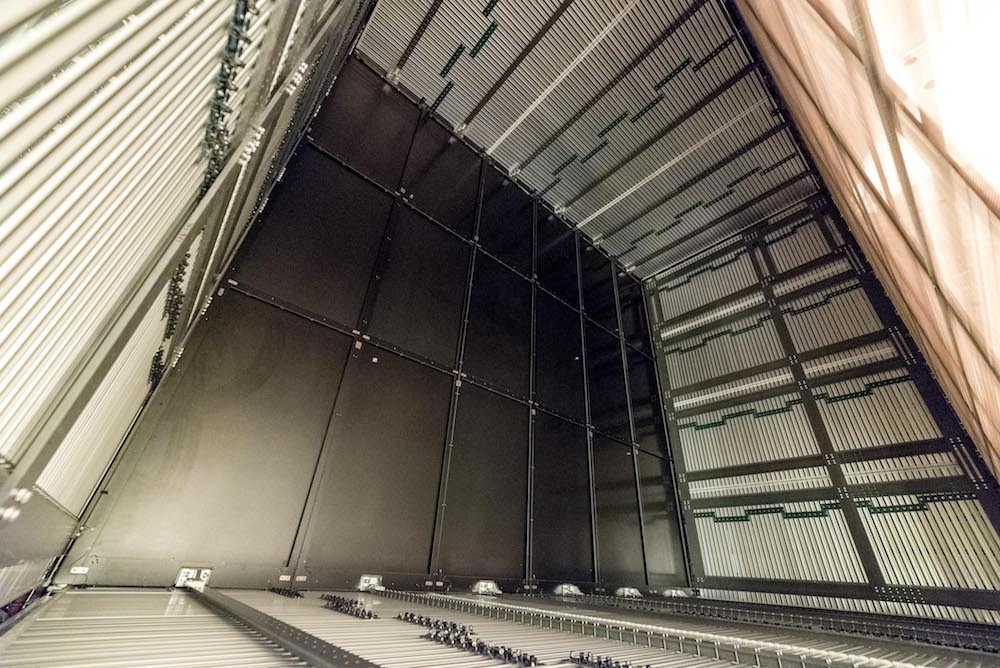
\includegraphics[width=0.8\textwidth]{protoDUNE-SP_TPCHV}
\end{dunefigure}

%%%%%%%%%%%%%%%%%%%%%%%%%%%%%%%%%%%%
\subsection{Summary of Construction and Operation}
\label{sec:fdsp-hv-protodune-summary}

The \dword{pdsp} \dword{hv} components underwent %some level 
various levels of preassembly offsite prior to transport and final assembly in the \dword{pdsp} clean room adjacent to the cryostat.

Parts for the top and bottom \dword{fc} frames were procured and test fit at Stony Brook University before being shipped to CERN for module assembly in a clean room about \SI{5}{km} away from the detector hall.
Fully assembled modules were transported individually to the detector hall for storage until installation. CERN provided the \dwords{gp} for the top and bottom \dwords{fc} as well as the field shaping profiles for all \dwords{fc}.

%\dword{ewfc} frame parts were acquired and test fit at Louisiana State University before being sent to CERN. The \dword{ewfc} frames were sent fully assembled, whereas the field-shaping profiles were installed and voltage divider boards mounted in the same CERN clean room facility. CERN provided the field-shaping profiles and, in the case of the top and bottom \dword{fc} units, the ground planes, while Louisiana State University provided all the voltage divider boards.

Louisiana State University provided all the voltage divider boards, then procured and test fit the \dword{ewfc} frame parts before shipping them fully assembled to CERN.
These profiles and the voltage divider boards were installed in the same CERN clean room facility as the other \dword{fc} components.

%\fixme{ I rewrote this because it was very inconsistent with how we defined things for DUNE - some of this is unavoidable due to the difference in size and that is explained in the text where necessary. And I used lower case descriptors here so that there is no confusion with the capitalized definitions for the DUNE CPA - SRM}
Argonne National Laboratory shipped the \dword{cpa} material to the detector hall as single preassembled resistive panels held in a FR4 frame - a \dword{cpa} module. 
In the clean room adjacent to the \dword{pdsp} cryostat, three \dword{cpa} modules were mechanically and electrically connected to produce a \dword{cpa} panel. %unit 
%\fixme{panel assembly?}
The \dword{cpa} panels (one of which is pictured in Figure~\ref{fig:cpa_panel-complete}) were first assembled horizontally, and then lifted and rotated to a vertical orientation where they were paired to make a 6.0 m $\times$ 2.3 m \dword{cpa} plane, as shown on the left in Figure~\ref{fig:cpas-in-cryostat}.
%\fixme{make sure we know how APA is defined in terms of planes, panels, etc.}
%\fixme{took out reference to APA size and put the size in meters -- krw}

At this point two top and two bottom \dword{fc} modules were brought to the clean room to be lifted, rotated to vertical, and attached to the \dword{cpa} plane. 
%\fixme{same question. Anne}
%\fixme{what is the question here? -- krw} 
%Once the load was transfered onto the \dword{cpa}, 
To fit through the \dword{tco} the top \dwords{fc} were suspended from their support at the top of the \dwords{cpa} plane to hang vertically, and the bottom \dwords{fc} were folded up and temporarily attached to their top \dword{fc} counterparts.
The resulting CPA-FC assemblies were rolled onto the central bridge beam inside the cryostat and subsequently deployed. 

Also in the \dword{pdsp} clean room, the preassembled \dwords{ewfc} %panels 
were assembled into the \dword{ewfc} planes (four endwalls/plane). %end wall).
Although not a component of the \dword{fd} design, 
the beam plug was installed onto its corresponding module %here 
%\fixme{"Panel" is not defined in table for FC components. The beam plug was installed into what? and below: replaced panel with module}
%\fixme{yes, panel == module in my language. Changed to module here.  -- krw}
before the beam-right, upstream \dword{ewfc} was built.
An electric hoist lifted the top %panel 
module to a height at which the next %panel 
module could be wheeled underneath and connected via FRP plates.
The hoist then raised the pair and the procedure would continue in this way until the \dword{ewfc} was four %panels 
modules tall.
The load of the assembled endwall was then transfered to a trolley on a transport beam, which allowed it to be pushed into the cryostat onto the appropriate bridge beam.

The TPC components of \dword{pdsp} were installed first for the drift space to the right of the delivered beam (beam-right), and then for the beam-left drift space.
The \dwords{apa} and the \dword{cpa} array were locked into position along their respective bridge beams, then the bridge beams were locked into their positions along the drift direction.
Next, the two \dwords{ewfc} were moved and rotated into their upstream and downstream positions to bridge the gap between the vertical edges of the corresponding \dword{apa} and \dword{cpa}.
The \dwords{ewfc} loads were transfered onto the \dword{apa} and \dword{cpa}  bridge beams, which freed the intermediate bridge beam for top and bottom \dword{fc} deployment.
Two mechanical hoists were used to lower (raise) the bottom (top) \dword{fc} to bridge the gap between the horizontal edges of the \dwords{apa} and \dwords{cpa}.
Finally, the HV cup was connected on the downstream \dword{cpa}, and the HV feedthrough was lowered through the cryostat penetration to make contact with the cup.

During the cooldown and \dword{lar} filling, a \dword{fc} termination power supply was used to supply $-$\SI{1}{kV} to the cathode and monitor the current draw of the system.
As the system cooled from room temperature to \dword{lar} temperature, the resistance increased by $\sim$10\% consistent with expectation.
Once the LAr level exceeded the height of the top ground planes, the voltage was ramped up to the nominal voltage.
After some evidence of leakage current localized to the warm side of the system, about 1 week was spent commissioning the HV delivery system.
The next ramp up to the nominal cathode voltage went flawlessly with no signs of anomalous current draws.
This level of high stability was maintained for about a week before small excessive current `blips', each persisting for no more than a few seconds, were observed.
The data suggests these blips were originating on the power supply side of the chain and not inside the TPC.
The magnitude of the excess current during such events increased over the subsequent 3 weeks from 1\% to 20\%.
The duration of the excessive current draws developed over this period as well, lasting up to 1 hour in some cases.
At this point, charge deposition onto one particular ground plane as well as the beam plug was observed in coincidence with the excess current draw from the power supply.
This type of activity was experienced periodically throughout the duration of the \dword{pdsp} beam run.

There was some evidence the power supply was introducing instabilities towards the beginning of the beam run.
We replaced the power supply midway through the run, which provided much more stability on the warm side of the \dword{hv} system.
However, some instabilities inside the TPC remained.
These came in the form of (i) fast discharges ($\sim$10 ms in duration) and (ii) persistent excessive current draw from the PS with accompanying excessive current detected on a ground plane and the beam plug.
The frequency of both classes of instabilities increased over time after the system was powered on, until a steady state of about 10 fast discharges/day and an instance of persistent current excess approximately once every 4 hours was achieved.
Nonetheless, during operation, the \dword{hv} system was able to consistently achieve >95\% uptime (manual quenching takes about 10 minutes), as shown in Figure \ref{fig:protoDUNE-SP_beamRunSum_HV}.

In some cases, when other parts of the system were down, the \dword{hv} system was turned off momentarily to allow the system to relax in case of some charging up that induces instabilities, and this is reflected as larger dips in the uptime.
During moments when the rest of the subsystems (including the beam) were stable, the moving 12-hour \dword{hv} uptime fluctuated between 96\% and 98\%.

\begin{dunefigure}[ProtoDUNE-SP HV performance during the test beam run.]
{fig:protoDUNE-SP_beamRunSum_HV}
{The performance of the high voltage system across the test beam period. The top panel shows the drift field delivered to the TPC, the middle panel indicates HV cuts during periods when the system is not nominal (some periods not visible due to their short timescale), and the bottom panel shows the moving 12-hour uptime of the \dword{hv} system based on these \dword{hv} cuts.
}
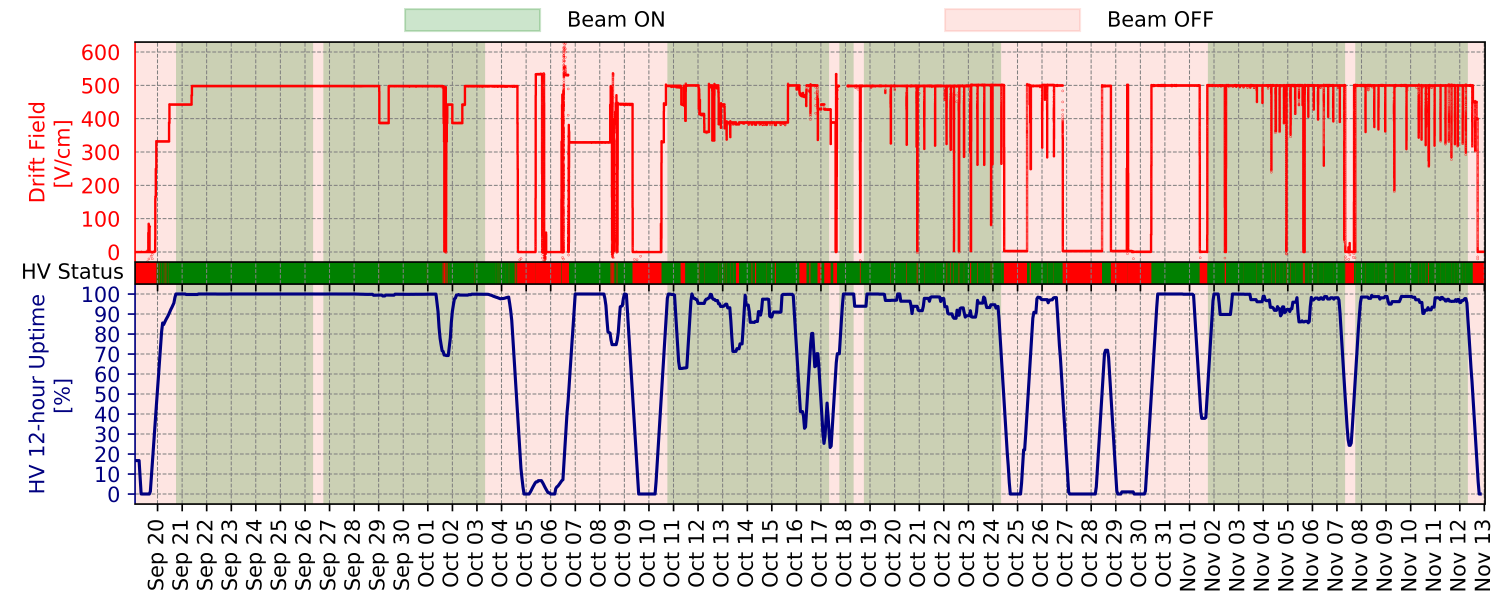
\includegraphics[width=\textwidth]{protoDUNE-SP_beamRunSum_HV}
\end{dunefigure}

The uptime during the week starting Oct. 11 is lower than the following 3 beam ON weeks because excessive currents were addressed differently between these periods.
In the beginning the excessive currents were left to exist until they quenched themselves.
Afterwards the voltage was ramped down until all current draws returned to nominal and then the voltage was brought back up.
Implementing automated controls to quench the excess current instead of relying on human intervention should increase the uptime, and such controls are currently being developed.

%\fixme{TOADD:}
%\begin{itemize}
%\item beam-run conditions/operations (``streamers'' exist, costs about 10 minutes per 4 hrs of operation)
%\begin{itemize}
%\item uptime \% during beam on periods (>90\%, needs to be calculated still)
%\end{itemize}
%\end{itemize}

%%%%%%%%%%%%%%%%%%%%%%%%%%%%
\subsection{Lessons from ProtoDUNE}

\label{sec:fdsp-hv-protodune-lessons}
The \dword{pdsp} HV experience was, in general, very encouraging, having demonstrated 
an ability to operate the TPC with a drift field of \spmaxfield{}. % was demonstrated.
However, throughout the run the system experienced various instabilities, the sources of which are %in the process of being investigated further
still under investigation.
Systematic study of these instabilities is underway.

%%%%%%%%%%%%%%%
\subsubsection{Design}
\label{sec:fdsp-hv-protodune-lessons-design}

The success of \dword{pdsp} validated the general design of the DUNE HV system - however various opportunities for improvement during its construction and operation were found. In particular,

\begin{itemize}
\item adopt a ``pot-style'' filter resistor design (with input and output cables on the same end) %would 
to prevent leaks from causing interventions for refilling;
%\item raising the cable insert to the HV feedthrough above the cold insulation space (if space allows); in the event the cable needs to be removed from the feedthrough, there is danger of moisture freezing on the walls and preventing good electrical contact. 
\item raise the HV feedthrough cable insert to be above the cold insulation space, if space allows (to allow cable removal while preventing moisture to enter and freeze on the walls, which could affect electrical contact);
\item add toroid signals %would be a welcomed addition 
to the feedthrough; and
\item improve stability by increasing the distance between the \dwords{gp} and field-shaping profiles and eliminating direct paths for potential surface currents.
\end{itemize}

%It is worth noting, the instrumented ground planes on the top and bottom field cages proved to be a valuable source of information during moments of instability. Furthermore, having a dedicated data acquisition system to readout the signals from the ground plane monitoring system, beam plug current monitor, and power supply read back at a rate of 20 kHz upon a trigger, provided very useful information for diagnosing the high voltage behavior inside the TPC. This system was not run continuously, but requires significant disk space to store the data it acquires.

The instrumented \dwords{gp} on the top and bottom \dwords{fc} proved invaluable for collecting information during moments of instability.
A dedicated \dword{daq} read out the signals from the \dword{gp} monitoring system, the beam plug current monitor, and the power supply at a rate of \SI{20}{kHz} on a trigger provided useful information for diagnosing the HV behavior inside the TPC.
%This system was not run continuously, since it requires significant disk space to store the data it acquires.
This system was not operated continuously due to correspondingly large data disk storage requirements.
Toroid signals from the \dword{hv} filters were also helpful in localizing sources of instability, specifically for distinguishing issues on the warm side from issues inside the \dword{tpc}.
%As mentioned above, investigations into the weak point of the system that introduces any additional path to ground, enabling excessive current draws, are underway.
%Given the consistent location of this ground path, it is more likely due to an undesired feature that was inadvertently introduced than a design flaw.
%There is also some evidence\footnote{Current excesses were much more frequent during periods when the beam halo increased the number of tracks traversing the TPC on the same side as the apparent weak point.} that the rate at which energy is deposited into the LAr impacts the rate of instabilities, which would be good news for DUNE.

As mentioned, undesired current draws implicated unknown but consistent grounding pathways, these weak points evident with an increase in the number of tracks traversing a \dword{tpc} during periods with increased beam halo.  Given the consistent location of the ground path, these weak points are likely inadvertent features rather than design flaws. There is some evidence that the rate at which energy is deposited into the \dword{lar} impacts the rate of instabilities, which would be good news for DUNE.  %edit by demuth



%%%%%%%%%%%%%%%
\subsubsection{Production, Handling and Quality Control}
\label{sec:fdsp-hv-protodune-lessons-assy}

The production and handling of HV components must be approached with %sufficient 
great care to avoid scratching and potentially compromising the electrical components. %or introducing scratches and other sharp edges.
%The aluminum field-shaping profiles are particularly prone to acquiring scratches if they are not packaged and handled in such a way to avoid direct contact with other profiles and materials.
Part production should be carried out in such a way to avoid introducing sharp edges wherever possible.
The corners of the ground plane panels had to be smoothed after some buckling was introduced during the pressing process, and a number of support hinges and clevises had sharp features removed by polishing.
The aluminum field-shaping profiles are particularly prone to scratches and must be packaged and handled so as to avoid direct contact with other profiles and materials.
%Kapton strips separated the profiles and the FRP of the FC frames as they were being inserted to avoid scratching and removal of the profile coating.
Kapton strips were used to separate the profiles from the FRP of the FC frames as they were being inserted to protect against scratching or removal of the profile coating.
Any scratches found in the FRP beams were covered with epoxy to prevent fibers from escaping into the \dword{lar}.

Various \dword{qc} tests were conducted on \dword{hv} modules and individual components at every step: %of the construction:  
part procurement, assembly, integration, and installation.
%Individual components or assembled submodules that were shipped to another facility had their previously administered QC tests repeated to ensure nothing was compromised during transport. 
To ensure that nothing was compromised during transport, QC tests were repeated on individual components and assembled pieces after shipping. 
Resistance between steps on the voltage divider boards were measured and verified to be within specification both after their production at LSU and after they were shipped to CERN.
Once the voltage divider boards were mounted onto an assembled FC module, the resistance between adjacent profiles was measured to verify sound electrical connection.
In a similar way, the connections between CPA modules and between CPA and FC modules were verified after integration.
%A predetermined, detailed \dword{qc} plan across the construction phase provided valuable cross checks.

The scale of DUNE will make some dedicated \dword{qc} tools very useful.
It was a tedious process to measure each voltage step individually several times each.
For example, designing a rig that can latch onto the \dword{fc} modules in such a way to make contact with all electrodes and control their voltages independently, would allow for an automated loop across all steps.
Such dedicated equipment and automated procedures will be useful for application to a full \dword{spmod}.

%%%%%%%%%%%%%%%
\subsubsection{Assembly and Installation}
\label{sec:fdsp-hv-protodune-lessons-assy}
The \dword{pdsp} experience allowed for a realistic estimation of the time involved to produce various \dword{hv} components for a \dword{spmod}.
The time involved for \dword{pdsp} was approximately as follows:
\begin{itemize}
\item FC module assembly - 1.5 days/module with 2 workers,
\item EW module assembly - 1.5 days/module with 2 workers,
\item CPA Plane - 2 days/Plane with 4 workers,
\item CPA Plane + FC integration - 1 day/assembly with 4 workers,
\item EW building - 4 hours/wall with 4-6 workers.
\end{itemize}
During installation there were some concerns about various alignment issues with the \dword{tpc}, but essentially all issues were corrected once the entire detector was in place.
The \dword{pdsp} installation sequence had the beam right drift volume deployed before the beam left.
Asymmetries in the weight distribution before the beam left drift was deployed produced subtle misalignments which propagated throughout the entire detector.
The process of connecting individual endwall modules to build an endwall exposed another alignment issue.
The first endwall turned out significantly bowed initially.
A tool was built to adjust the angle between adjacent modules, which straightened out the wall.
The tool was also used while connecting modules for the remaining three endwalls and no significant bowing was observed.

%\subsubsection{Performance}
%\label{sec:fdsp-hv-protodune-lessons-perf}
%There is a clear weak point in the \dword{pdsp} \dword{hv} system, which appears to be near the top, upstream corner of the cathode.
%Investigations are underway to identify the nature of this weak point, but successfully operating the detector with >95\% uptime despite this weak point was a reassuring exercise.
%\begin{itemize}
%\item Continuous operation at -180kV on the cathode
%\item Fast discharges
%\item "Streamers" (no impact on TPC signals observed, some evidence on PDS)
%\end{itemize}

%%%%%%%%%%%%%%%%%%%%%%%%%%%%
\subsection{Future R\&D}
\label{sec:fdsp-hv-protodune-RD}

A number of proposed R\&D items arose from the \dword{pdsp} experience.  These include:
\begin{itemize}
\item Evaluate the charge and discharge behavior of the \dword{uhmwpe} caps on the end of the profiles compared to metallic capped profiles.  The goal is to check if the PE endcaps contribute to HV instability. \fixme{define acronyms - uhmw, pe. Anne  make sure all terms are defined, caps is one}
\fixme{switched UHMWPE to the dword version.  Caps has been used elsewhere in the document. -- SEL}
%\item Compare the HV stability of 90-degree-bent profiles with capped profiles at a right angle. The goal is to check if the bent profiles are more stable for HV performance than a capped design meeting at a right angle.
\item Compare the HV stability of bent versus capped profiles at 90 degrees. %The goal is to check if the bent profiles are more stable for HV performance than a capped design meeting at a right angle.
\item Evaluate resistive versus metallic caps.  If the \dword{uhmwpe} caps are %shown to be 
problematic, find an alternative solution to maintain separated \dword{fc} modules.
%\fixme{maintain segmentation of the FC modules? Like, to keep them separated?}
%\fixme{Yes, to keep them separated. -- sel}
\item Study the surface-charging behavior of the \dword{fc} insulation structures.  Evaluation of general insulator performance for \lartpc{}s, including charge-up effects and geometry, remains an outstanding task.  In this test, the goal is to find out if any geometrical feature or surface treatment can reduce HV instability.
\item Evaluate higher-resistivity Kapton films.  The goal is to check the feasibility of increasing the surface resistivity of the cathode plane up to 1~G$\Omega$/square.  The task includes verifying the lamination quality on \frfour sheet and production availability.
\item Perform further simulation of  HVS discharge behavior.   While modeling other \dword{fc} designs and DUNE will take considerable effort, % the possibility of 
understanding the source of instabilities or exposing any design weaknesses would be worthwhile. %makes this a worthwhile endeavor.
\end{itemize}

%%%%%%%%%%%%%%%%%%%%%%%%%%%%%%%%%%%%%%%%%%%%%%%%%%%%%%%%%%%%%%%%%%%%
\section{Interfaces }
\label{sec:fdsp-hv-intfc}

\fixme{ docdb refs still not working - giving to final edit team.}


%% \begin{verbatim}
%% Format for 
%% @techreport{bib:docdb6754,
%% title = "{DUNE FD Interface Document: DP CRP to Joint High Voltage}",
%% author = {{Duchesneau, D. and Pietropaolo, F. and Yu, B.}},
%% year = {2018},
%% note = "\url{http://docs.dunescience.org/cgi-bin/ShowDocument?docid=6754&version=1}"
%% }
%% \end{verbatim}

The High Voltage System has the largest surface area on the TPC and interfaces with many other systems.  Table~\ref{tab:HVinterfaces} summarizes the interfaces with other consortia, highlights the key elements, and provides the links to the existing interface documents.

The two most important mechanical interfaces are with the DSS and the APA.  The entire weight of the CPAs, \dword{ewfc},  and half the weight of the top and bottom FC is supported by rails provided by the DSS.  The other half of the T/B FC weight is transferred to the APAs through latches mounted on the APAs. All CPAs and most of the FC modules are also transported along the DSS rails to their final positions. The DSS rails ultimately determine the final locations of the CPAs and FCs on the TPC.

Electrically, since the APAs are at the detector ground, all HVS field cage termination and failsafe circuits are connected to the APAs.  All cables used for the FC termination pass through the APA frame, to connect to the SHV cables provided by the CE through the CE signal flanges.  The CE Consortium also provide HVS the FC termination power supplies.




\begin{dunetable}
[\dword{hv} system interfaces]
{p{0.25\textwidth}p{0.5\textwidth}l}
{tab:HVinterfaces}
{High Voltage System Interface Links }   
Interfacing System & Description & Linked Reference \\ \toprowrule
\dword{dss}  &  Support, positioning, and alignment of all \dword{cpa}, \dword{fc} modules inside the cryostat both warm and cold & %\citedocdb{nnnn}{n} 
\\ \colhline
\dword{apa} & \dword{fc} support (top, bottom, and end wall) on \dword{apa} frames; Mounting of FC termination filter boards and \dword{fc} failsafe terminations; 
%% EDs are APA's responsibility (BY)
%% Mounting of the electron diverter boards.
& \cite{bib:docdb6673} 
\\ \colhline
\Dword{ce} & \dword{fc} termination wire connectors on CE feedthrough flange, \Dword{fc} termination wires routed with CE cables & \cite{bib:docd6739} 
 \\ \colhline
\dword{pds} & Mounting of PD calibration flash diffusers and routing of their fibers to \dwords{cpa}; Possible \dword{tpc} coated reflector foil on \dwords{cpa}. & \cite{bib:docdb6721} 
 \\ \colhline
Facility & Locations and specifications of the \dword{hv} \fdth ports; gas and \dword{lar} flow velocities and patterns. & \cite{bib:docdb6985}  
\\ \colhline
Calibration & \dword{fc} openings for the calibration laser heads & \cite{bib:docdb7066}
\\ \colhline
\Dword{cisc} & \dword{hv} vs. \dword{lar} level interlock, sensor locations in high field regions, cold/warm camera coverage, \dword{hv} signal monitoring, etc. & \cite{bib:docdb6787} 
 \\ \colhline
\Dword{itf} & Storage buffer, inspections/tests, repackage for underground delivery & \cite{bib:docdb7039} 
 \\ \colhline
Physics & Requirements: range of operating drift field, uniformity of the drift field; Supply detector geometry and \efield{} map. & \cite{bib:docdb7093} 
 \\ 
\end{dunetable}

%%%%%%%%%%%%%%%%%%%%%%%%%%%%%%%%%%%%%%%%%%%%%%%%%%%%%%%%%%%%%%%%%%%%
\section{Production and Assembly }
\label{sec:fdsp-hv-prod-assy}

%%%%%%%%%%%%%%%%%%%%%%%%%%%%
\subsection{Power Supplies and Feedthroughs}
\label{sec:fdsp-hv-supplies-feedthroughs}

We plan to buy commercial power supplies, %will be commercially procured, 
for example through Heinzinger. The \dword{hv} cable is commercially available.

The power supply is tested extensively along with the controls and monitoring software.  Features to be included in the software are:
\begin{itemize}
\item The ability to ramp, or change, the voltage, set the ramp rate and pause the ramp. % The rate and an ability to pause the ramp shall be included.  
In previous installations, the ramp rate was typically between \SIrange{60}{120}{V/s}.
\item An input for a user-defined current limit.  This parameter is the current (I) value at which the supply reduces the voltage output to stay below the current limit.  The current-limiting is done in hardware.
\item An input for a trip threshold.  At this current reading, the program would reduce the voltage output through software.  In previous experiments, the trip function in software would set the output to \SI{0}{kV}.
\end{itemize}
Additionally, the software must
record the current and voltage read-back values with a user-defined frequency, as well as any irregular current or voltage events.

The \dword{hv} feedthroughs and filters are custom devices.  %For fabrication, t
The feedthrough can be made by collaborators, or we can send the design to a company for fabrication.  Raw materials such as stainless steel, \dword{uhmwpe} rods, and flanges are available as stock items and must be machined to make a feedthrough.  Similarly, the resistors, steel or aluminum, and insulator material for the filters can be bought from stock.  The feedthroughs and filters require testing before being delivered to the ITF. 

%%%%%%%%%%%%%%%%%%%%%%%%%%%%
\subsection{Cathode Plane Assembly}
\label{sec:fdsp-hv-prod-cpa}

Commercial vendors or university collaborators will produce the component parts of the \dword{cpa} array. 
They will package the parts into kits, each to contain the parts for a single \dword{cpa} Panel (three \dword{cpa} Units). The parts in each kit are 
%for the following items:
%\fixme{clearly define cpa vs assembly, mentioned earlier}
\begin{itemize}
\item manufactured \frfour \dword{rp} frames, % packed into kits for a single \dword{cpa} panel (three \dword{cpa} units),
\item carbon-impregnated Kapton-coated \dwords{rp} and \dwords{fss},
\item \dword{hv} cable segments and wire jumpers making up the \dword{cpa} \dword{hv} bus and \dword{rp} interconnects,
\item resistor boards connecting the \dwords{rp} to \dwords{fss} (for raising the \dword{rp} HV by \SI{1.5}{\kV}),
\item machined brass tabs for connecting \dwords{rp}, \dword{hv} bus, and \dwords{fss}, and
\item top, bottom, and exterior edge profiles and associated connection hardware.
\end{itemize}
The kits are sent to the production factories, the locations of which will be determined later.  
The %basic 
\dword{cpa} construction unit for installation into the \dword{spmod} at \surf is a pair of \dword{cpa} panels called a \dword{cpa} plane. The production factory thus ships assembled \dword{cpa} panels to \surf where they are paired in the underground clean room at \surf{}. % to form a \dword{cpa} plane. 

The most basic element of the \dword{cpa} 
is a \dword{rp} mounted in a machined slot in the top, bottom and sides of \frfour frames.  

%\fixme{what's written is correct - we don't make CPA modules for DUNE  - we make CPA Units which are composed of 2 of the former CPA modules.  CPA is defined as Cathode Plane Assembly which is historical and we are stuck with it - it means the whole thing - SRM}

%\fixme{This next paragraph is confusing. Let's talk through it. Anne}

%\fixme{Here's Anne's rewrite of orig p, please check:} 
There are three different \dword{rp} types  -- an upper, which has as its top frame the \dword{cpa} mounting bracket and \dword{topfc} hinge, a middle, and a lower, which has as its bottom frame a \dword{botfc} hinge.  

Pairs of \dwords{rp} are bolted together and pinned to form \dword{cpa} units of size \SI{1.2}{\m} $\times$ \SI{4}{\m} for shipment. Three types of pairings are constructed to make a full six-\dword{rp}, \SI{12}{\m} tall \dword{cpa} panel: (1) an upper and a middle, (2) two middle , and (3) a middle and a lower.

The order in the shipping crate from top to bottom is middle-and-lower, middle-and-middle, and upper-and-middle.   Two \dword{cpa} panels are shipped together in one crate; they are paired at \surf to form one \dword{cpa} plane.  The \SI{10}{\kt} \dword{spmod} requires 100 upper, 100 lower and 400 middle \dwords{rp} to make up the 100 \dword{cpa} panels (50 \dword{cpa} planes) of the \dword{tpc}.

The \dword{cpa} units are assembled horizontally on a smooth, flat table to provide a highly stable surface, enabling assembly to meet the dimensional requirements of \dword{cpa} construction.  
%\fixme{the fact that they are assembled this way shouldn't be the reason they meet the dimenstional requirements. Please reword.}
In addition to the frames and \dwords{rp}, 
\dword{fss} strips are mounted on the exposed sides of the \frfour frames, aluminum profiles are attached to the exterior edges of the upper and lower \dwords{rp}, 
%\fixme{"top (and bottom) of the upper (and) lower"?} 
and cables are attached to the \dwords{rp} to form segments of the \dword{hv} bus.  

A \SI{6}{\m} \dword{pdsp} \dword{cpa} panel and a \SI{12}{\m} \dword{pdsp} \dword{cpa} panel are shown at Ash River Laboratory in Minnesota, USA,  in Figure~\ref{fig:12m-cpa}.
%\fixme{end Anne's rewrite = This has too much cut - RKP - discuss}
%\fixme{ this is all consistent with the table of definitions at the beginning - SRM}

%There are three different types of these \dwords{rp} -- an upper, which has as its top frame the \dword{cpa} mounting bracket and \dword{topfc} hinge, a middle, and a lower, which has as its bottom frame a \dword{botfc} hinge.  
%Two such \dwords{rp} are bolted together and pinned to form a \dword{cpa} unit of size \SI{1.2}{\m} $\times$ \SI{4}{\m} for shipment.  These \dword{cpa} units are assembled horizontally on a smooth, flat table to meet the dimensional requirements of \dword{cpa} construction.  In addition to the frames and \dwords{rp}, %\dword{fss}s 
%\dword{fss} strips are mounted on the exposed sides of the \frfour frames, aluminum profiles are attached to the top and bottom of the upper and lower modules, and cables are attached to the \dwords{rp} to form segments of the \dword{hv} bus.  The shipment \dword{cpa} Unit comes in three varieties in order to make a full \SI{12}{\m} tall \dword{cpa} Panel.  These are : (1) an upper \dword{cpa} \dword{rp} module attached to a middle module, (2) two middle modules connected, and (3) a middle module attached to a lower module.  The \dword{cpa} Unit order in the shipping crate from top to bottom is middle-and-lower, middle-and-middle, and upper-and-middle.  These 3 \dword{cpa} Units make up one \dword{cpa} Panel.  Two \dword{cpa} Panels are shipped together in one crate - these two Panels will be paired at \surf to form a \dword{cpa} Plane.  For the \SI{10}{\kt} \dword{spmod}, there are 100 upper \dword{cpa} \dword{rp} modules, 100 lower \dword{cpa} \dword{rp} modules and 400 middle \dword{cpa} \dword{rp} modules that make up the 100 \dword{cpa} Panels and 50 \dword{cpa} Planes of the \dword{tpc}.
%A comparison of a \SI{6}{\m} \dword{pdsp} \dword{cpa} Panel and a \SI{12}{\m} \dword{pdsp} \dword{cpa} Panel is shown at Ash River Laboratory in Minnesota, USA,  in Figure~\ref{fig:12m-cpa}.

\begin{dunefigure}[\dwords{cpa} at Ash River]{fig:12m-cpa}{A \SI{12}{\m} DUNE-SP \dword{cpa} mockup Panel and a %smaller 
half-height \SI{6}{\m} \dword{pdsp} panel mockup at Ash River, Minnesota.}  %closest panel 6m, each strip separated by 2m, this image taken in the pit at Ash River (where NOvA modules were stacked/glued.)
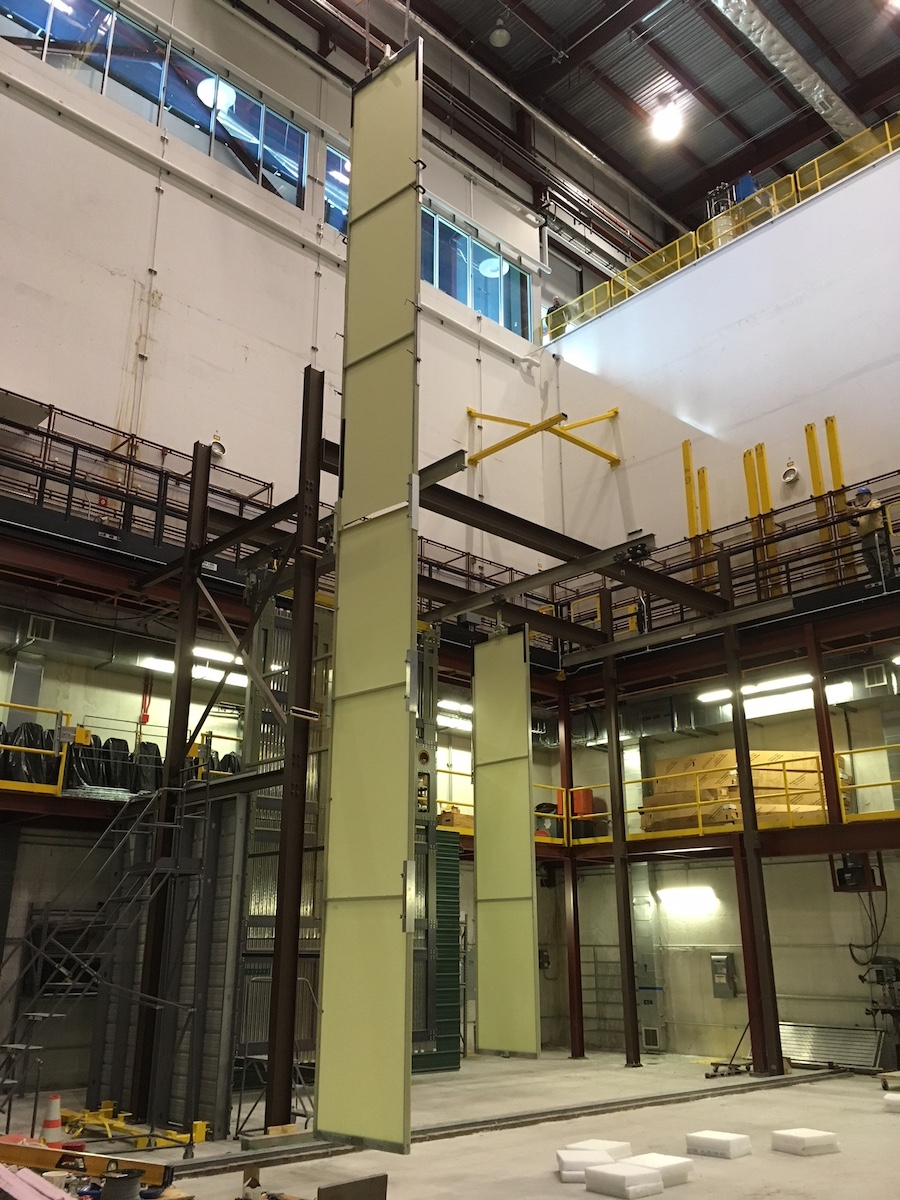
\includegraphics[width=0.5\textwidth]{12m-cpa}
\end{dunefigure}

%%%%%%%%%%%%%%%%%%%%%%%%%%%%
\subsection{Field Cages}
\label{sec:fdsp-hv-prod-fc}

%\fixme{Is it one field cage with top, bottom and endwall portions, or are they separate field cages? We should be consistent. Anne. There are two, one on each side of the CPA}

\subsubsection{Top and Bottom Field Cages}

%Discussion of parts procurement, assembly, and testing.
Firms that specialize in the machining of fiberglass components for electrical applications will produce the FRP and \frfour components of the top and \dwords{botfc}, as was successfully done for \dword{pdsp}. All parts are to be machined in the absence of water to minimize absorbed water in the \dword{tpc}, and then cleaned with a lacquer thinner. 
%\fixme{why is absence of water important?}
All the machined edges except the small circular holes are to be coated with translucent epoxy. The stainless steel and aluminum components will be produced in university and commercial machine shops. University groups will likely fabricate the voltage divider boards and \dword{fc} and \dword{cpa} connection boards.
%The voltage divider boards will be provided by Louisiana State University, and the boards used to make the \dword{fc}/\dword{cpa} connection will be provided by Kansas State University.

The FRP frame assembly process primarily consists of fastening together FRP I-beams with FRP threaded rods and hex nuts,  securing them with a limited and specified torque to avoid damage to the threads. A detailed view of one of these connections is shown in Figure~\ref{fig:tbfc3}.

\begin{dunefigure}[Top and bottom \dword{fc} module frame assembly]{fig:tbfc3}{The figure shows the procedure for connecting the cross beams to the main I-beams for the \dword{topfc}. Left: A display of the components of each connection, which (from top to bottom) are the threaded rods, the spacer tubes, washer plates, the hexagonal nuts, and an L-shaped FRP brace. An intermediate stage (middle) and final stage (right) of the assembly are also shown.}
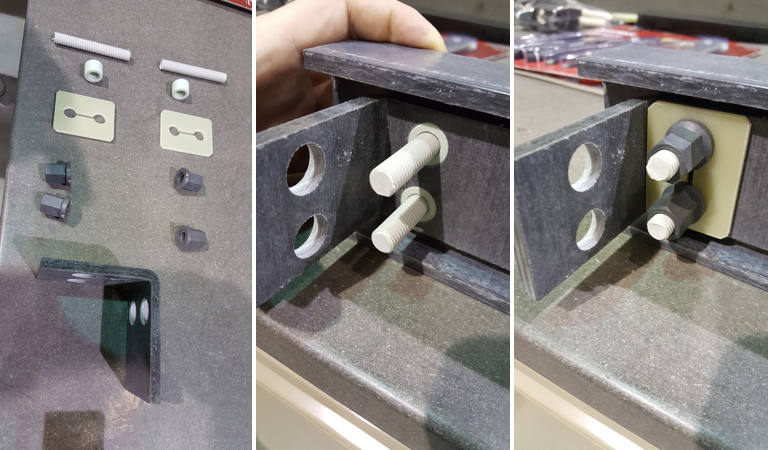
\includegraphics[width=0.70\textwidth]{tbfc3}
\end{dunefigure}
%\fixme{The relationship of the left figure to the other two is not clear to me. Caption needs work, too. Would like to discuss. Anne. Believe this is addressed -RKP}

Prior to sliding each profile into the FRP frame, the holes %should be (should be? Anne changed to are)
are covered with Kapton tape to avoid damage to the profile coating. An end cap is attached to each profile using plastic rivets, then the profiles are aligned against an aligment fixture running the length of the \dword{fc}. After securing each profile to the frame, the tension in the mounting screws is adjusted to remove any angular deflection in the extended portion of the profile.

The \dwords{gp} are attached to the \SI{10}{\cm} stand-off I-beam sections with threaded rods and a machined plate. The copper strips are connected to adjacent modules at the same locations. Care must be taken to avoid bending the corners of the \dwords{gp} toward the profiles, particularly on the \dword{cpa} side of of the module.

%%%%%%%%%%%%
\subsubsection{Endwall Field Cages}

For the \dwords{ewfc} all FRP plates are commercially cut to shape by water jet, as are the cutouts in the FRP box beams. % are also cut by water jet. 
Holes that accommodate G10 bushings are reamed in a machine shop. FRP frames are pre-assembled to ensure proper alignment of all FRP parts and %matching of 
holes. The profiles are not inserted at this stage. The FRP modules are hung off of each other by means of interconnecting FRP plates to ensure accurate alignment.

Next, parts are labeled and the frames are taken apart. All components are cleaned by pressure washing or ultrasonic bath. All cut FRP surfaces are then coated with polyurethane, which contains the same main ingredient as the FRP resin, allowing it to bond well to the FRP fibers. Final panels are constructed from cleaned and inspected parts. In order to ease assembly, which requires access to both sides of a module,
a dedicated assembly table has been manufactured that allows convenient module rotation. 

Figure~\ref{fig:endwall_assy_rot_table} pictures a partially assembled \dword{ewfc} FRP frame on the assembly table.
\begin{dunefigure}[Endwall assembly table]{fig:endwall_assy_rot_table}{Assembly table with partially assembled \dword{ewfc} module. Box beams, cross beams, and slots for mounting of aluminum profiles are visible. (Credit: LSU)}
 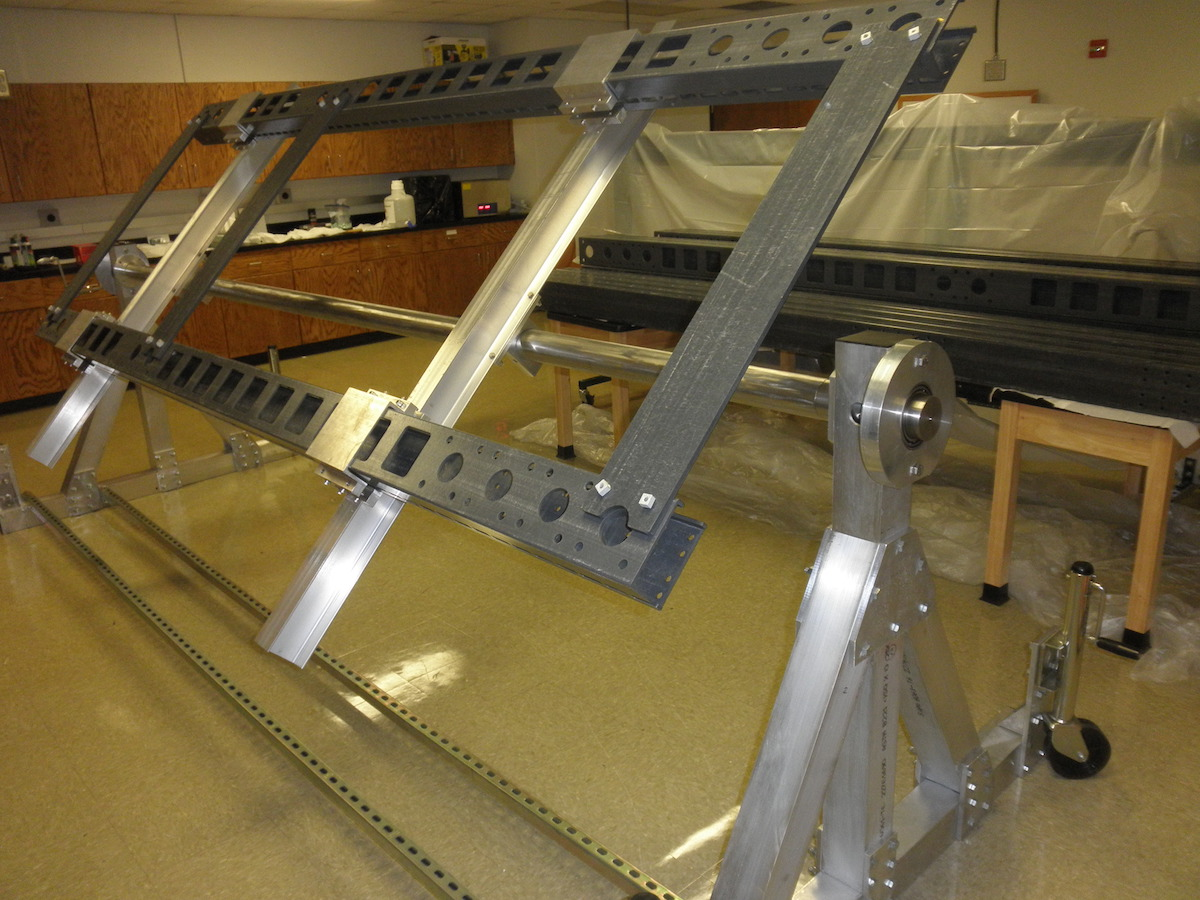
\includegraphics[width=0.8\textwidth]{endwall_assy_rot_table}
 \end{dunefigure}
%\fixme{caption should identify main features in image. Anne}
The FRP box beams are sandwiched between \SI{1.27}{\cm} (\num{0.5}\,in) thick FRP panels that are held on one side by means of G10 bushings and rods with square nuts.
On the other side M10 stainless steel bolts, which are clearly visible in Figure~\ref{fig:endwall_assy_detail},  
engage with large slip nuts that are inserted into the aluminum profiles. The profiles 
are pulled towards a \SI{2.5}{\cm} thick FRP plate located 
on the inside of the box beam.
%

\begin{dunefigure}[Endwall assembly detail]{fig:endwall_assy_detail}{%Left: Side view of upper part of a top \dword{ewfc}  module.
Top and center \dword{ewfc} module frames hanging. (Credit: LSU)}
%\includegraphics[width=0.48\textwidth]
%{fc_endwall_detail_side}
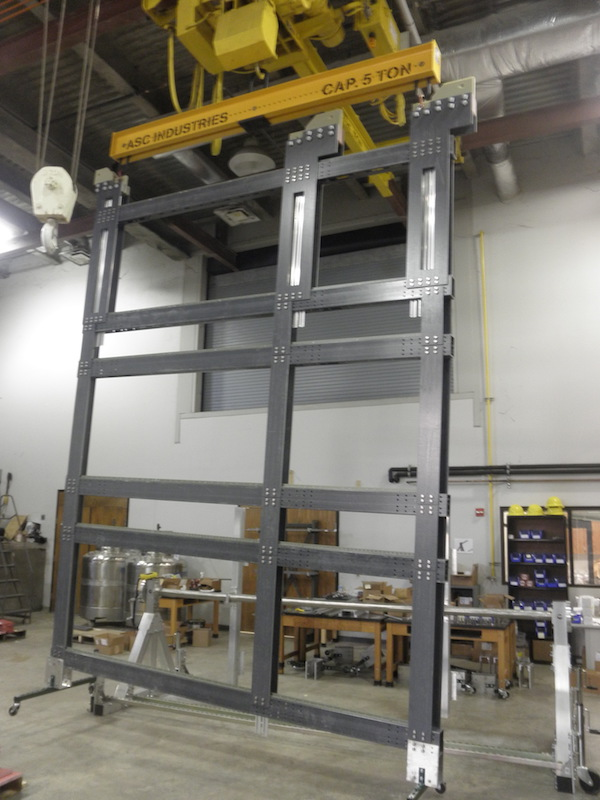
\includegraphics[width=0.7\textwidth]{3_fc_endwall_frames_hanging}
\end{dunefigure}


Aluminum profiles are inserted into the cutouts of the box beams and attached with screws and stainless steel slip nuts to L-shaped FRP brackets that are mounted on the FRP box beams. 
%\fixme{refer back to figure \ref{fig:tbfc3}? No, different one -RKP} After this, the resistive divider boards are mounted to the profiles using brass screws that engage with stainless steel slip nuts inside the profiles.

%%%%%%%%%%%%%%%%%%%%%%%%%%%%
\subsection{Electrical Interconnections}
\label{sec:fdsp-hv-prod-interconnect}

All electrical fasteners and wires used on the \dword{cpa} arrays and \dword{fc} are produced
to specification by commercial vendors and packaged with the \dword{cpa} or \dword{fc} modules.  
As discussed above in Sections~\ref{sec:fdsp-hv-prod-cpa} and~\ref{sec:fdsp-hv-prod-fc}), 
this includes the \dword{hv} cable segments, as well as wire jumpers, machined brass
tabs, etc.

University shops will produce and test circuit boards for %DUNE 
\dword{hv} interconnections according to the same design used for \dword{pdsp}.  The \dword{fc} voltage dividers were produced for \dword{pdsp} at Louisiana State University, and the boards for \dword{cpa} frame bias and \dword{cpa}-\dword{fc} connections were produced at Kansas State University.
%\todo{What about the \dword{fc}-to-\dword{apa} boards?} 
Both institutions have created custom test apparatuses for verifying proper operation of the boards at full voltage and over-voltage conditions, keeping the boards free of solder flux and flux-remover.  These institutions may scale up production and testing by the required order of magnitude for the \dword{spmod}, or share this work with other institutions, whichever best meets the needs of the project. %Each board is free of solder flux and flux-remover. (moved sentence up)

%%%%%%%%%%%%%%%%%%%%%%%%%%%%
\subsection{Production Safety}
\label{sec:fdsp-hv-prod-safety}

Production of the \dword{fc} panels and resistor-divider boards will involve collaboration technical, scientific, and student labor and  does not present unusual industrial hazards. The \dword{hv} consortium will work closely with each production site to ensure that procedures meet both Fermilab and institutional requirements for safe procedures, personal protective equipment, environmental protection, trained materials handling, and training. The vast majority of production part fabrication will be carried out commercially and shipping will be contracted through approved commercial shipping companies. Prior to approving a site as a production venue, each site will be visited and reviewed by an external safety panel to ensure best practices are in place and maintained. 

Testing of the \dword{hv} feedthrough will be done in a closed cryostat leading to no exposed high voltage.  Special attention will be given to the grounding between the power supply and cryostat.  This type of testing setup has been used successfully, and safely in the testing of \dword{hv} feedthroughs for years.

\clearpage
%%%%%%%%%%%%%%%%%%%%%%%%%%%%%%%%%%%%%%%%%%%%%%%%%%%%%%%%%%%%%%%%%%%%
\section{Quality Control, Transport, and Installation}
\label{sec:fdsp-hv-transport}
%\fixme{ I added text here and in 1.5.1 for the QA plan and implementation of QC and 1.5.2 for transport and handling - SRM}
The \dword{hv} consortium has developed a comprehensive \dword{qc} 
%\fixme{I think this should be qc. Anne}
plan for the production, shipping and installation of the \dword{spmod} \dword{hv} components. %has been developed 
It is based partly on \dword{qc} procedures developed and implemented on \dword{pdsp} and on the \nova experiment's successful use of barcode tagging for identifying and tracking detector components.  Inventory tagging and tracking each component is crucial. %Anne added last sentence to flow into the following content
%\fixme{I'd change 'elements' above to 'components'. Done - RKP}

For DUNE, the purity requirements of the \lar place restrictions on the introduction of material into the cryostat, precluding either permanent tags or ink or paint markings on the detector.  We will implement a system of temporary tags containing QR or barcodes  in which the tags are removed when their codes are scanned.  %The tag selection requirements are that 
The tags will be large enough and of bright enough color to be seen from both ends of the cryostat.  We are considering %A particularly suitable choice is to use 
bright yellow \textit{cattle tags} -- plastic tags of about 10-12 square inches ($\sim$ 70 cm$^{2}$) on which a unique QR\texttrademark{} or barcode can be printed; they can be purchased very inexpensively in quantities of hundreds or thousands.

%%%%%%%%%%%%%%%%%%%%%%%%%%%%
\subsection{Quality Control (QC)}
\label{sec:fdsp-hv-transport-QC}

Power supplies used in a \dword{spmod} will be tested before installation.  Output voltages and currents must be checked on a known load. 

The feedthrough and filters should be tested at the same time, preferably with the planned power supply.  The feedthrough must be tested to hold the required voltage in \dword{tpc}-quality \dword{lar} ($\tau\geq$\SI{1.6}{ms}) for several days.  The ground tube submersion and \efield{} environment of the test setup should be comparable to the real field cage setup or more challenging (e.g., the test liquid level can be lower than %DUNE's 
that in the \dword{spmod} but not higher).  Additionally, the feedthrough must be leak-tight to satisfy cryogenics requirements.

The \dword{qc} process for mechanical components starts at the production factories by attaching a cattle tag with a unique code to each production element.  A file linked to each code contains the individual measurements and properties contained in the \dword{qc} checklists for that element.  The following is an example of how this system will be implemented for the \dword{cpa} components:

\begin{enumerate}
\item During assembly, \dword{qc} checklists are filled out electronically using a smart phone or tablet.  Once a \dword{cpa} Unit 
%\fixme{2-module unit not clear; use terms per table \ref{tab:cpaparts}. Anne}
%\fixme{fixed this - SRM}
is completely assembled and all checklists are complete, a coded temporary cattle tag is attached and scanned, linking the checklist information to the code on the tag. (The \dword{cpa} Unit's individual parts are not tagged separately.)
\item %Each 2-module Unit has attached to it a tag with a unique code linking its QC checklists - individual parts for a 2-module Unit are not tagged separately.   
A shipping crate will contain six %2-module 
\dword{cpa} Units, each with its removable coded tag, plus any included hardware packages, each with a coded sticker.
\item A coded label on the shipping crate (paper sticker) will %contain 
identify the contents of the crate (six codes + codes of hardware packages). 
%\fixme{2 hw pkgs? anne} \fixme{the number of hardware packages is flexible - we will probably put everything in 1 package, but could separate into multiple packages for more clarity of installation procedures - SRM} The code on the label is only used only for shipping purposes and for inventory purposes at the \dword{itf}.
\item In the \surf clean room, the first \dword{cpa} Panel is assembled -- a coded tag is attached to the \dword{cpa} Panel and scanned.  The three individual \dword{cpa} Unit tags are then scanned and removed, linking them to the \dword{cpa} Panel code.
\item The same procedure is followed for the second \dword{cpa} Panel from the crate.  Each \dword{cpa} Panel now has a single tag attached it.
\item The %next step is to combine 
\dword{cpa} Panels are then combined into a \dword{cpa} Plane, and a single coded tag is attached to the \dword{cpa} Plane and scanned. % is attached to the Plane and scanned.  
The two individual \dword{cpa} Panel tags are then scanned, linking their codes to the that of the \dword{cpa} Plane. %Plane.
\item Top and bottom \dword{fc} modules 
%\fixme{this should be module; no fc unit is defined. Anne - done RKP}
are attached to both sides of the \dword{cpa} Plane, and  a single coded tag is placed on this \dword{cpafc} assembly identifying the codes of each of the four \dword{fc} modules %(4 tags) 
and the code of the \dword{cpa} Planes;  %CPA Plane (one tag) - 
these five tags are removed after scanning.  
\item When moving into the cryostat the code of the position tag on the \dword{dss} is scanned as well as the tag on the \dword{cpafc} assembly, then both tags %\dword{cpafc} 
are removed.
\end{enumerate}
At this point, %what is obtained is 
a sequence of linked codes associated with \dword{qc} checklists %that tell 
identify which CPA and FC modules %units 
are mounted in %the 
which \dword{dss} positions and no tagging material remains in the cryostat.  A similar sequence is anticipated for the production of the FC Top and Bottom units up to Step 6 and separately for the end walls.  
%\fixme{prev sentence unclear to me. Anne} 
%\fixme{I used the CPA assembly as an example - similar procedures are defined for the FC and EndWall assemblies - I don't know them exactly  - do we need to detail them as well or is this example good enough? - SRM}
At the completion of installation in the cryostat and before \dword{fc} top and bottom deployment, visual inspection will confirm the absence of any tags.

%%%%%%%%%%%%%%%%%%%%%%%%%%%%
\subsection{Transport and Handling}
\label{sec:fdsp-hv-transport-transport}

The HVS consortium has studied %issues of 
options for %the means of 
transportation from HVS production sites %factories 
to the \dword{itf} %along with the type of 
and packaging of the shipped elements. % were studied within .  
%The use of inexpensive, disposable crates to be used between factories and the ITF with transfer to reusable underground crates was compared to the use of just reusable underground crates with return to the factories of empty crates.  
We found that using reusable underground 
crates and returning them to the factories when empty is less expensive than using inexpensive, disposable crates for shipment from the factories to the \dword{itf},  
%It was found that the latter method was cheaper 
even with the extra shipment costs. %s of empty crates back to factories. 

We have identified a vendor that %was found which 
produces honeycombed PVC sheets of varying thicknesses that can be formed into crates. These %that 
can be loaded at the production sites, %factories, 
shipped to the \dword{itf}, and sent underground at \surf.  
As an example, %for the CPA, 
it will require 50 shipments of crates containing two \dword{cpa} Panels each to complete the \dword{spmod}.  %With the reusable underground crate scheme in place, only 20 crates are required to make the 50 shipments. 
The reusable underground crate scheme requires only 20 crates to make the 50 shipments. Similar reductions are obtained for the top and bottom \dword{fc} modules. 
%\fixme{that word unit again!! (anne asks: are these 'elements' really modules or portions of modules?) RKP- changed to modules}
%\fixme{ I didn't know how the top and bottom FCs were defining their components when I wrote this so I used the generic lower case units - it should be changed to be consistent with their definitions, just like the CPA descriptions should be consistent with the defs in the intro table - SRM}

Crates would be available at each factory at the start of production. %; as shipments are made and installation proceeds at \surf, empty crates are returned to each factory as required. (Anne thinks that text is unneeded)
%Inside the crates, individual assembly units are bagged and sealed at the production factory.  At SURF, the crates are lowered into the staging area outside the clean room where the crates are unpacked and the assembly units removed from their bags and taken into the clean room for installation. 
As production proceeds, individual assembly units are bagged and sealed inside them.
%\fixme{missing ITF stage?}
%\fixme{Yes - here it is - SRM}
When a full shipment of crates is ready at a factory, crates are sent by flatbed truck from the factory to the \dword{itf} at Rapid City, South Dakota.  The full crates are stored at the ITF until they can be received at SURF.  Some components may require QC and/or minor assembly procedures to be done at the \dword{itf} before shipping to SURF.

At SURF, the crates are lowered into the staging area outside the clean room where they are unpacked. The assembly units are removed from their bags and taken into the clean room for installation. Only cleaned assembly units are allowed into the clean room -- the crate is restricted to the staging area only. The empty crate is returned to the \dword{itf} and then sent back to a production factory for reloading. 

%\fixme{why the extra stop at the ITF?}
%\fixme{I assumed that there would be dedicated trucks used to ship items between ITF and SURF. If not, and the correct number of MT crates can be loaded at SURF for shipment to a factory, then the extra stop at the ITF is not needed - SRM}

%%%%%%%%%%%%%%%%%%%%%%%%%%%%
\subsection{Safety during Handling} % Safety}
\label{sec:fdsp-hv-transport-safety}
%\subsection{Assembly and Installation}
%\label{sec:fdsp-hv-install}

%\fixme{This section will discuss interaction of HV experts with
%Integration team, and reference the appropriate chapter/volume for further details.}

In the current installation scenario, no assembly activities are foreseen at the ITF site for any components of the HV system. Only visual inspection of the HVS modules will be performed to verify the integrity after shipping. This only requires the opening and the successive re-closing of the shipping crates. No specific safety procedures are associated with these operations. The HV consortium will coordinate procedures for underground handling with Technical Coordination.

%\fixme{Note to editors: It isn't clear to the consortium if the current installation plan requires this section, since ITF handling is conventional. If the section is included, we would like to have the correct phrasing as used by other consortia. -RKP, FP}

%%%%%%%%%%%%%%%%%%%%%%%%%%%%
\subsection{Installation and Integration}
\label{sec:fdsp-hv-transport-install}
%\subsection{Installation and Integration}
%\label{sec:fdsp-hv-integratio}
Installation of the components of the HVS starts with the downstream (non-TCO end) \dwords{ewfc}.  Two endwall "toaster" crates,  
%\fixme{why are they called toaster crates? And why can you bring crates into the cryostat? Anne}
%\fixme{They are toaster crates because the EndWall pieces are packed so that you can remove them one at a time like taking several pieces of toast out of a 4-slot toaster.  We decided to use crates that could be brought into the clean room and I think the idea is to wrap the toaster crates at the factory so that they are as clean as the Endwalls and can then go into the cryostat - SRM}
containing four endwall modules each, are transported into the cryostat.  Together they contain the eight individual modules that make up the  
downstream \dword{ewfc} for one drift volume. % between a \dword{cpa} plane  and an \dword{apa}.  

The modules are removed from their crates starting with the topmost unit and proceeding by attaching subsequent modules until the entire eight-module, \SI{12}{m} structure
%\fixme{1m can't be right - right, its 12 m} 
is hanging vertically from its support beam.  This is repeated for the remaining three assemblies, making up the full downstream \dword{ewfc}. %; in all, four eight-module assemblies.  

Next, the first of the 25 rows (counted lengthwise along the \dword{detmodule}) of \dword{apa}s and \dword{cpafc} assemblies are positioned in the order \dword{apa}, \dword{cpafc}, \dword{apa}, \dword{cpafc}, \dword{apa}.  Electrical and mechanical connections between the \dword{ewfc} and \dword{apa}s and the \dword{ewfc} and \dword{cpa} arrays are made.  At this point, deployment (unfolding) of the \dwords{topfc} and \dwords{botfc} %attached to the \dword{cpa} Planes 
occurs.  Once they % Top and Bottom FCs 
are latched at the \dword{apa} ends, and the FC termination connections are made and verified on the APAs, this \dword{tpc} row is complete.  Subsequent rows of \dword{apa}s and \dword{cpafc} assemblies are positioned sequentially, using the same procedure, completing the 25 rows. % of the TPC volume.  
Once the 25th row is in place, its \dword{topfc} %are 
is deployed, latching to the \dword{apa}s.  Before the \dword{topfc} is deployed, the upstream \dword{ewfc} crates are brought into the cryostat 
and the \dwords{ewfc} are built up from their crates in the same manner as the downstream ones. % - four 8-module Endwall assemblies between APAs and \dword{cpa} Planes.  
Once they %endwalls 
are in place and the \dwords{botfc} are deployed, the \dword{tpc} volume is enclosed. %finishing the TPC field cage volume of the detector. 
%\fixme{different from tpc volume?}
Finally, electrical and mechanical connections between \dwords{ewfc} and \dword{apa}s and between \dwords{ewfc} and \dword{cpa} arrays are made, completing all field cage connections in the \dword{tpc}.

%% added by BY
Compared with the time needed to install and verify the APAs, the CPA/FC modules installation is relatively simple and quick.  Since the deployment of the top and bottom FCs blocks physical access to the interior volumes, the installation scheme described above limits the access to the installed TPC components to only the outer row being installed.  An alternative installation scheme is being considered, which offers accessibility for much long period of time.  In this scheme, after the far \dword{ewfc} is completed, both APAs and CPA/FCs are installed into position along their DSS rails at their natural pace without deploying the FCs. This leaves the aisles between the CPAs and APAs free with floor in place in case access to previously installed TPC modules is needed.  Once nearly all APAs are installed, the floor boards are removed and FCs are deployed.   




%\fixme{to here 11/19 before meeting. Anne}
%\fixme{This is the order so far - SRM}

\begin{dunefigure}[\Dword{pdsp} \dword{cpa} plane before and after \dword{fc} attachment]{fig:cpas-in-cryostat}{Left: Completed \dword{pdsp} \dword{cpa} plane ready for \dword{fc} attachment. Right: Two completed \dword{cpa}-\dword{fc} assemblies in the \dword{pdsp} cryostat. The top and bottom \dwords{fc} with their \dwords{gp} attached are visible to the right of the cathode plane in their folded-up pre-deployment position.}
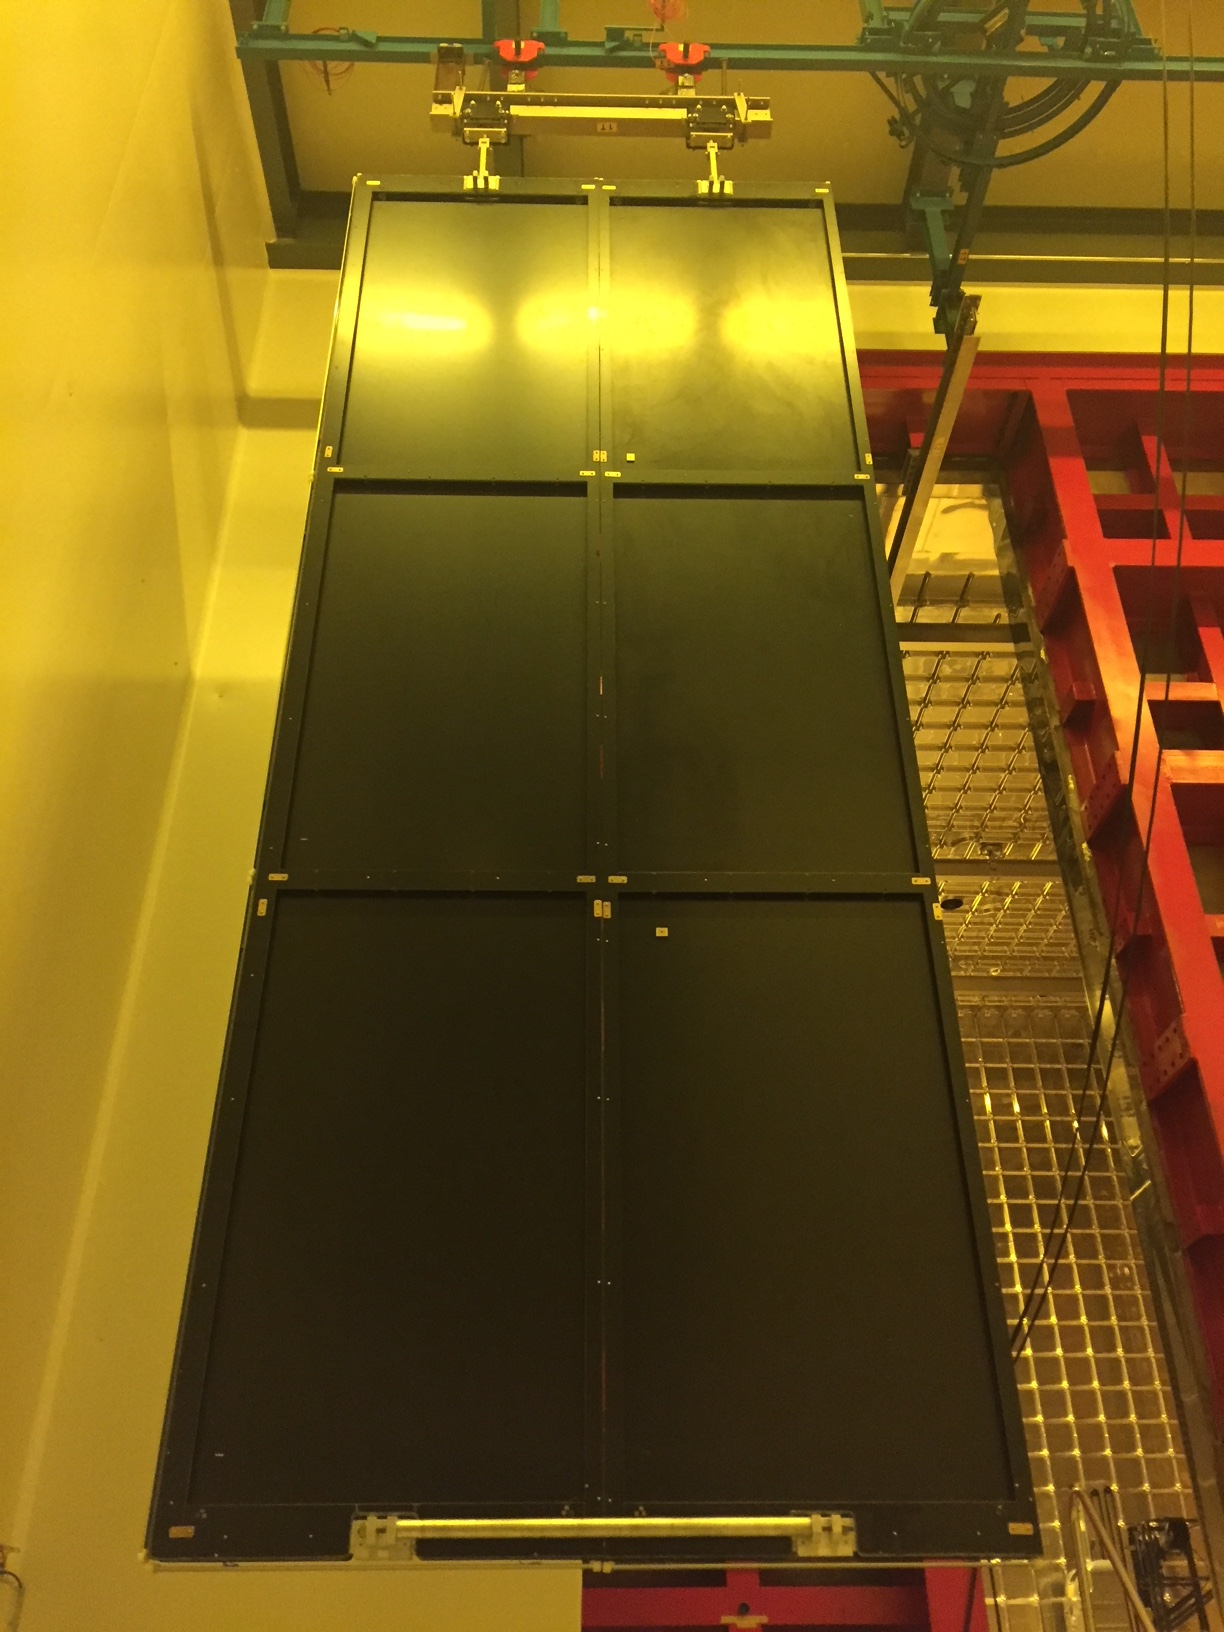
\includegraphics[width=0.45\textwidth]{lastcpa}
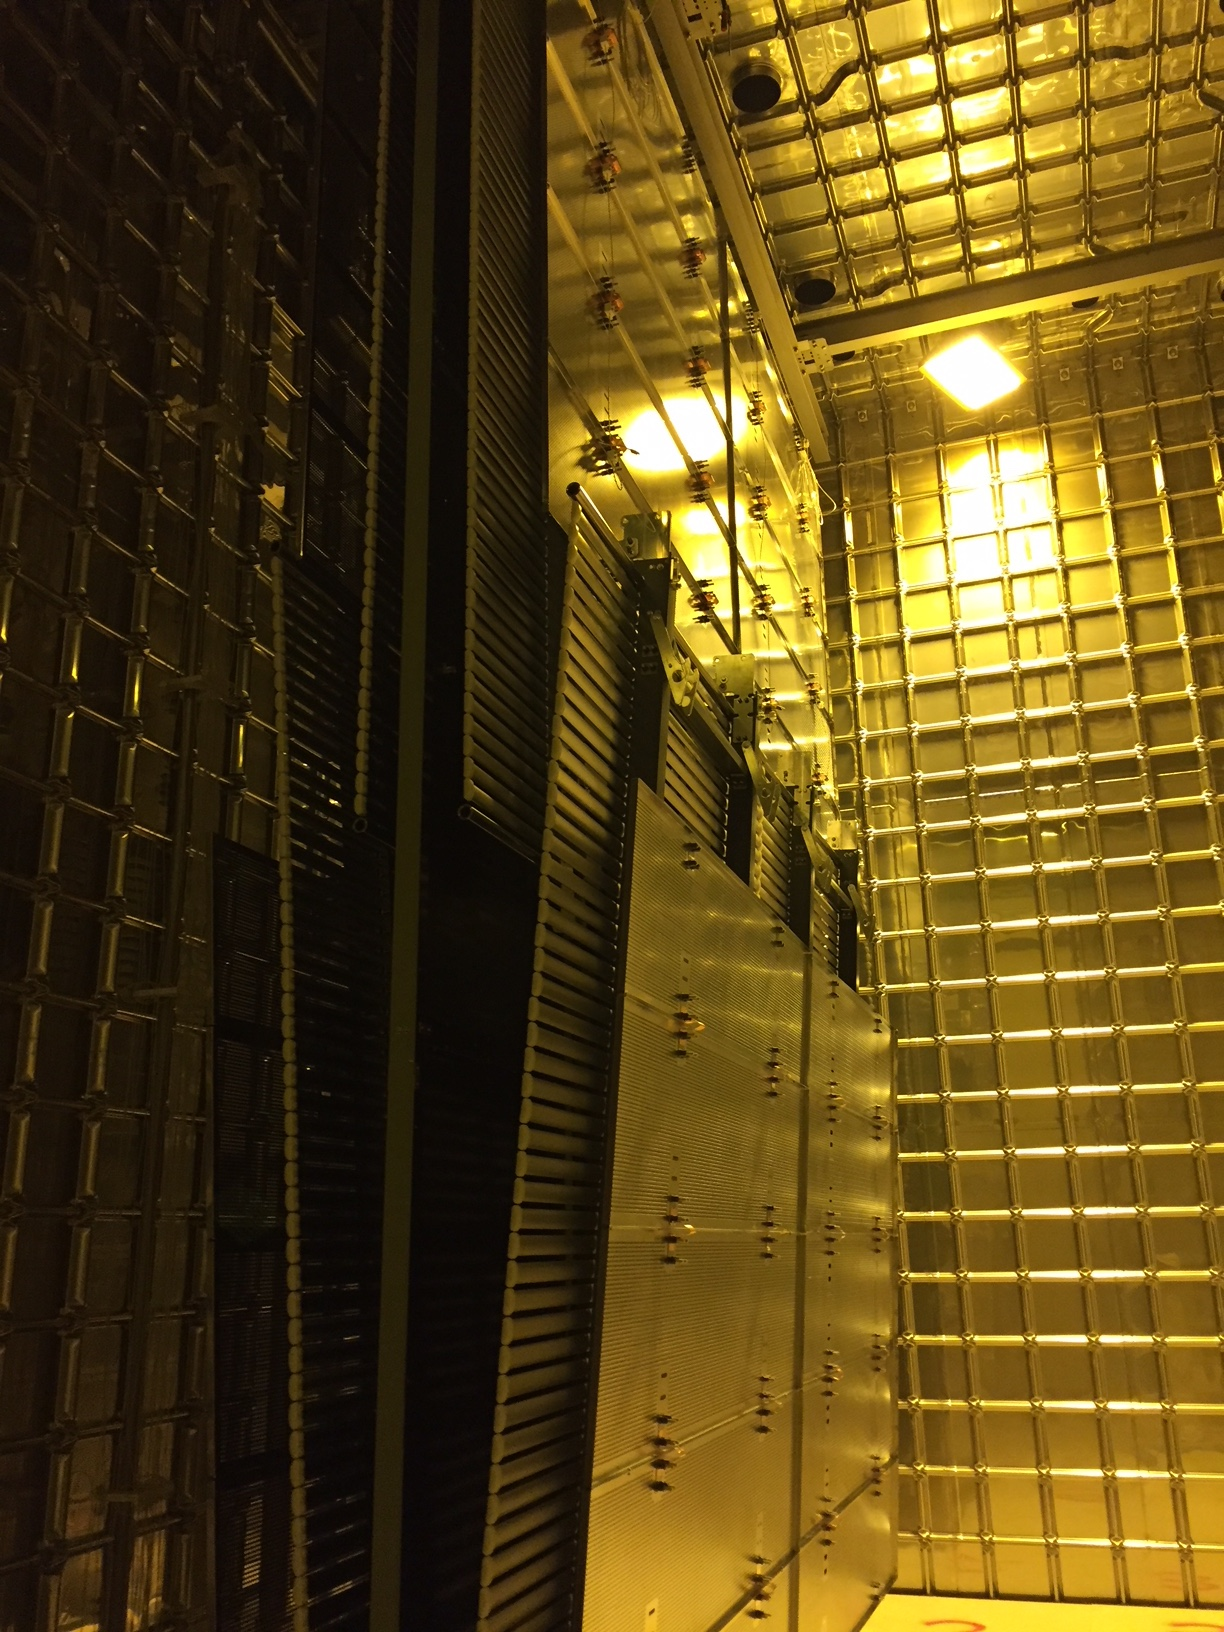
\includegraphics[width=0.45\textwidth]{2cpas-in-cryostat}
\end{dunefigure}

\begin{dunefigure}[\Dword{pdsp} \dword{ewfc} installation]{fig:EndwallInstall}{Completed endwall %in process of being 
during installation into \dword{pdsp} cryostat. In %the case of 
\dword{pdsp}, the individual endwall modules were connected to form the wall in the clean room before being pushed into the cryostat. %In the case of DUNE, 
For the \dword{spmod} the endwall will be built up inside the cryostat near its final position.}
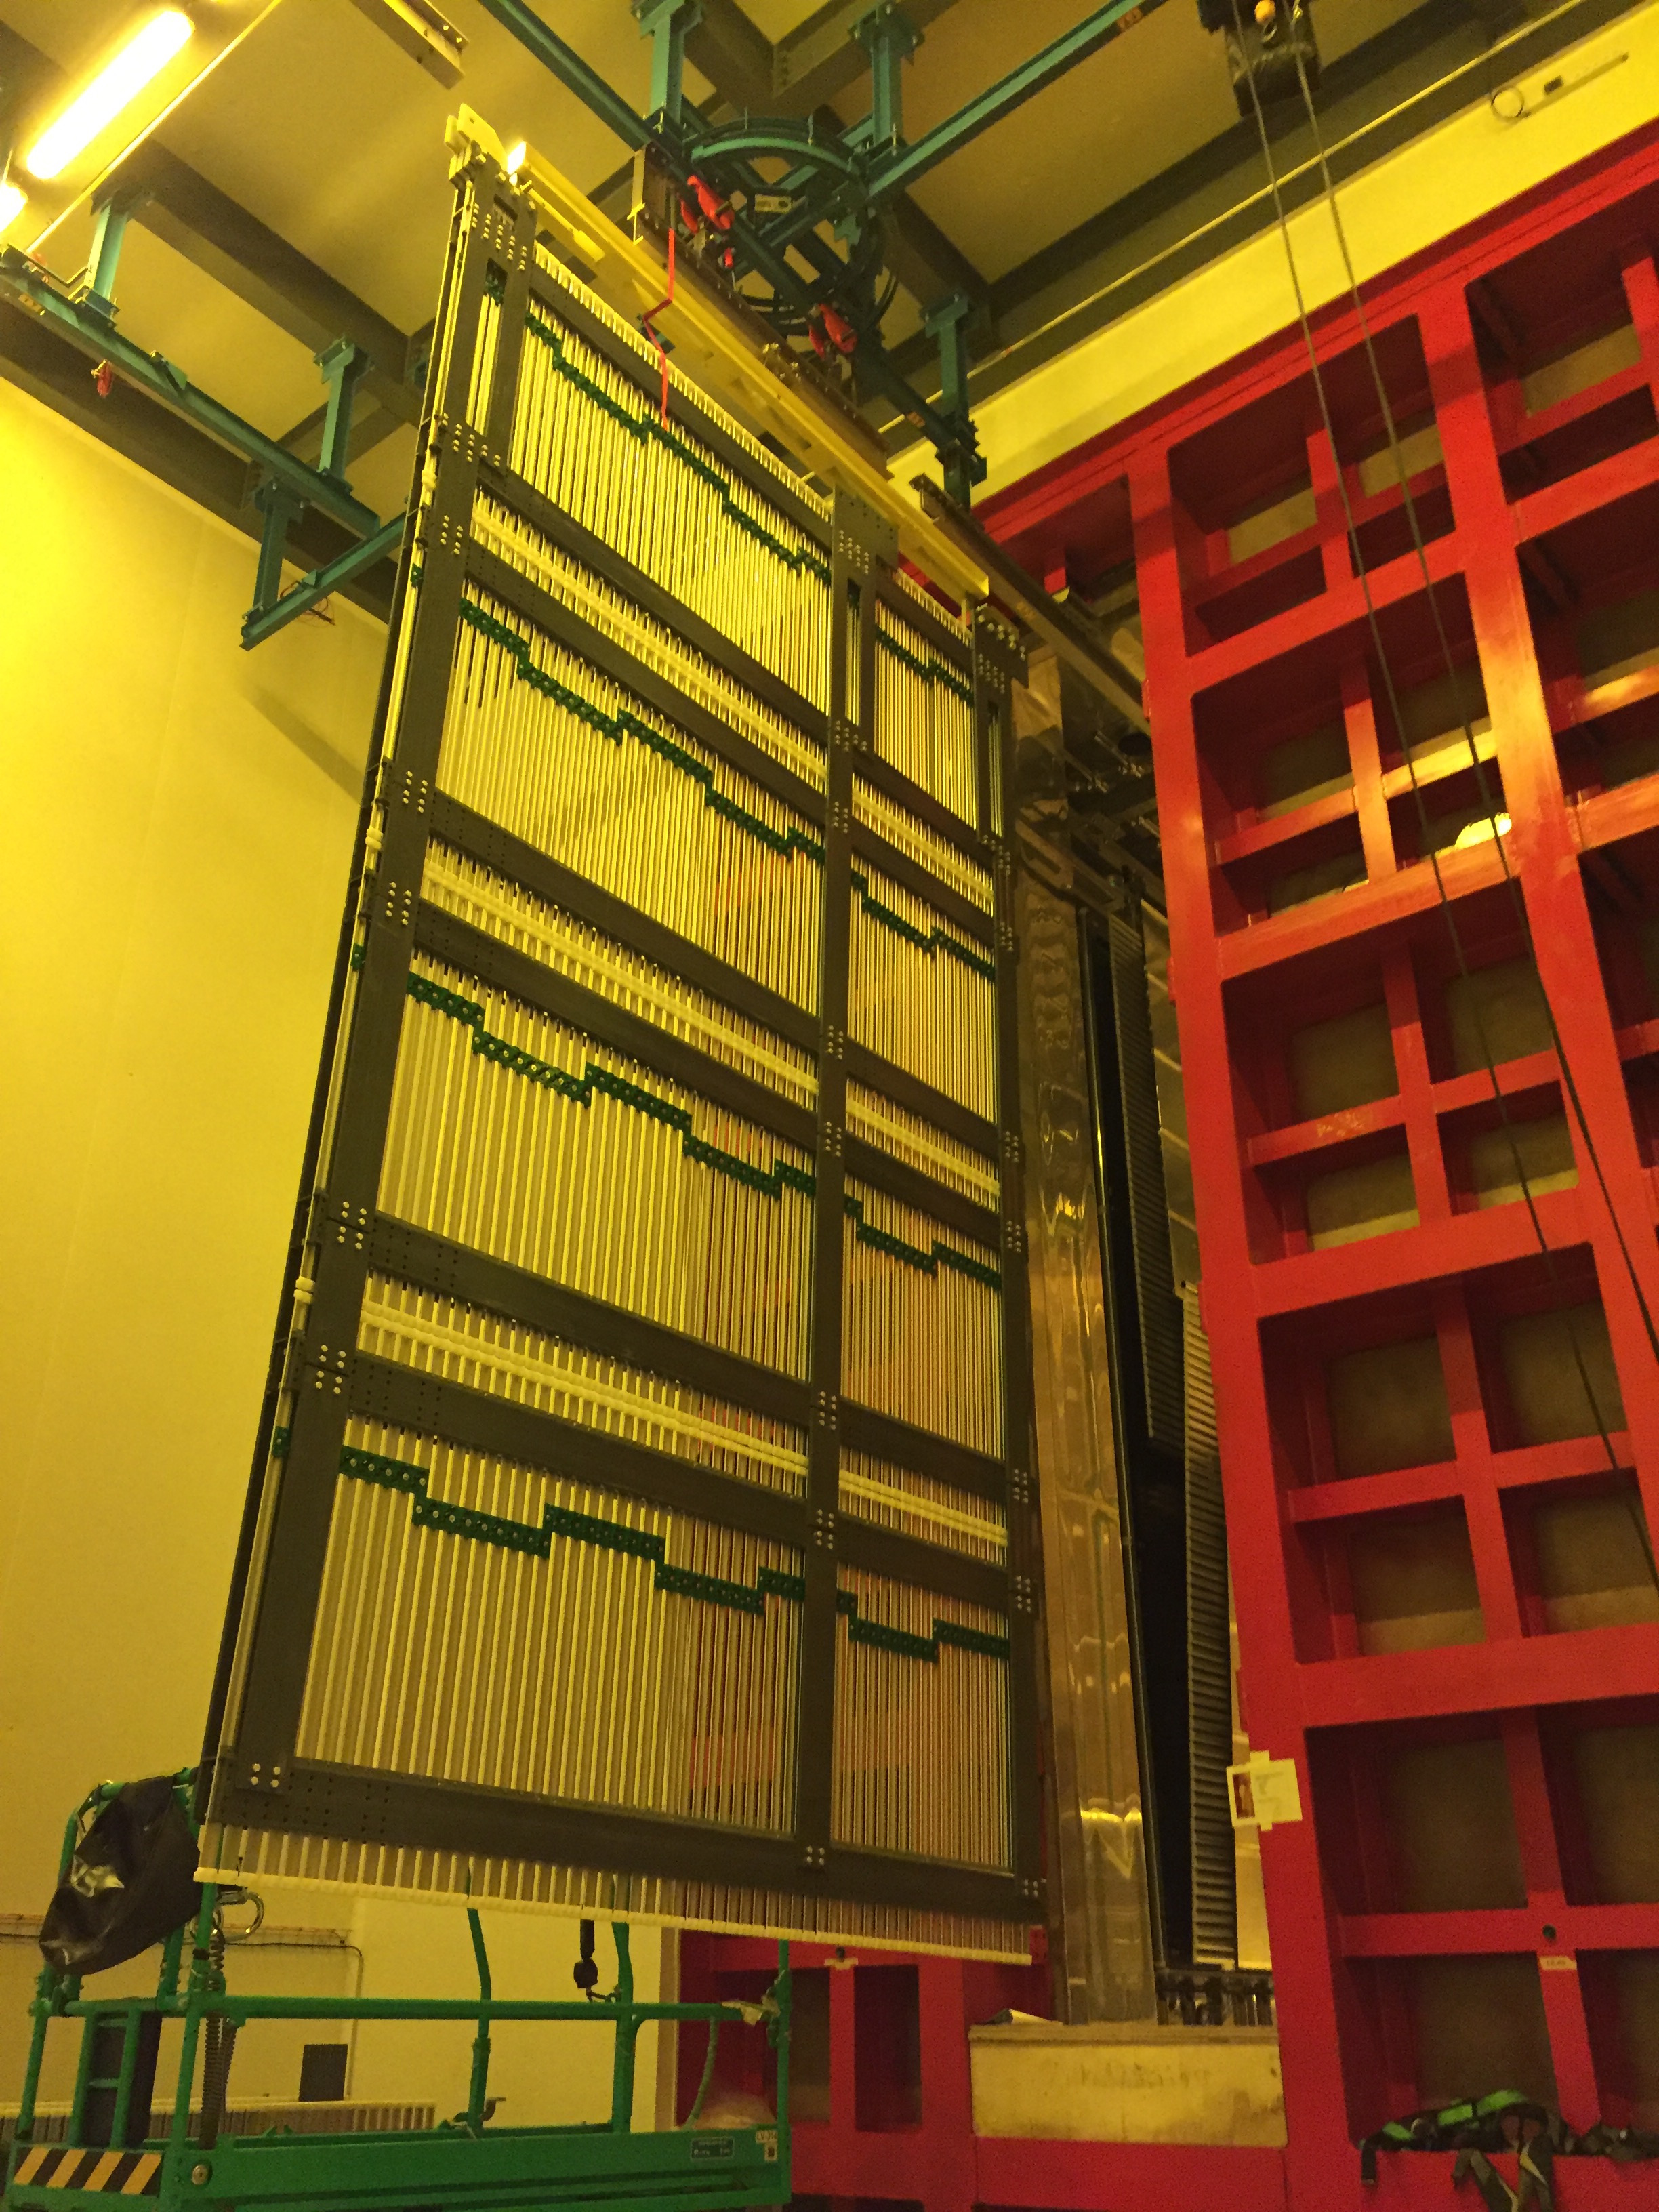
\includegraphics[width=0.45\textwidth]{endwall_and_tco.jpg}
\end{dunefigure}


\clearpage
%%%%%%%%%%%%%%%%%%%%%%%%%%%%%%%%%%%%%%%%%%%%%%%%%%%%%%%%%%%%%%%%%%%%
%\section{Quality Control (QC)}
%\label{sec:fdsp-hv-qc}
%\clearpage
%%%%%%%%%%%%%%%%%%%%%%%%%%%%%%%%%%%%%%%%%%%%%%%%%%%%%%%%%%%%%%%%%%%%
%\section{Safety}
%\label{sec:fdsp-hv-safety}
%\clearpage
%%%%%%%%%%%%%%%%%%%%%%%%%%%%%%%%%%%%%%%%%%%%%%%%%%%%%%%%%%%%%%%%%%%%
\section{Organization and Management}
\label{sec:fdsp-hv-org}

%%%%%%%%%%%%%%%%%%%%%%%%%%%%

\subsection{Institutional Responsibilities}
\label{sec:fdsp-hv-org-consortium}
The HVS consortium has consolidated 
all the institutions that have participated in the design, construction and assembly of the \dword{hv} systems for both \dword{pdsp}  and \dword{pddp}. 
%
%The consortium 
It currently comprises several USA institutions and CERN, %presently 
the only non-USA participant. As %in the case of 
for \dword{protodune}, CERN is heavily committed to a significant role in terms of funding, personnel, 
 and the provision of infrastructure for R\&D and detector optimization. Moreover, CERN will be responsible for a significant fraction of subsystem deliverables; as such  CERN is actively in search of additional European institutions to attract into the consortium. 
 
 In the \dword{hv} current consortium organization, each institution is naturally assuming the same responsibilities that it assumed for %the developments of 
\dword{pdsp} and \dword{pddp}.

The %present 
consortium organizational structure 
 includes a scientific lead (from CERN), a technical lead (from BNL), a \dword{tdr} editor (from \fnal), and a HVS design and integration lead ( from ANL). 
%  \fixme{structure or leadership? Anne. Refrased: FP}

%\fixme{I removed all the "currently"s -- it's the current consortium org. anne}
 The consortium is organized into working groups addressing the design and  R\&D phases of development, and the hardware production and installation.

\begin{itemize}
\item WG1. Design optimization for \dword{spmod} and \dword{dpmod}; assembly, system integration, detector simulation, physics requirements for monitoring and calibrations. %Conveners: Jeff Nelson, Vic Guarino, Bo Yu
\item WG2. R\&D activities, R\&D facilities. %Conveners: Francesco Pietropaolo, Ting Miao
\item WG3. \dword{sp}-\dword{cpa}: Procurement of resistive panels, frame strips, electrical connections of planes; assembly, \dword{qc} at all stages, and shipment of these parts. %Convener: Stephen Magill
%\fixme{too many QC's. And confusing. Procurement, assembly, QC at all stages, and shipment of these parts? Anne - Done RKP}
%\fixme{Not sure where this came from - do you want detailed list of duties or should it just be the name of the group? - SRM; Simplified: FP}
\item WG4. \dword{dp} cathode and ground plane:  material procurement; construction, assembly, shipment to ITF \dword{qa}, \dword{qc}.% Convener: Jae Yu
\item WG5.  modules: \dword{sp}-Top/Bottom-\dword{fc} module, \dword{sp}-EndWall modules , \dword{dp}-\dword{fc} modules: procurement of mechanical and electrical components, assembly and shipping to ITF . %Conveners: Thomas Kutter, Michael Wilking, Jeff Nelson, Jae Yu
%\fixme{ditto. Anne}
\item WG6. \dword{hv} supply and filtering, \dword{hv} power supply and cable procurement, R\&D tests, filtering and receptacle design and tests. %Conveners: Franco Sergiampietri, Sarah Lockwitz
\end{itemize}

%Merging of \dword{sp} and \dword{dp} activities is performed for the working groups where synergies have been identified: 
Taking advantage of identified synergies, some activities of the \dword{sp} and \dword{dp} working groups are merged:\dword{hv} feedthroughs, voltage dividers, aluminum profiles, FRP beams, and assembly infrastructure.

\begin{dunetable}
[Participating institutes]
{p{0.15\textwidth}p{0.75\textwidth}}
{tab:instit}
{Institutes participating in the HVS consortium}   
ID & Institution \\ \toprowrule%(Contact, E-mail) 

1 & CERN, Switzerland \\ \colhline%(Francesco Pietropaolo; francesco.pietropaolo@cern.ch) 
2 & Argonne National Lab, USA \\ \colhline%(Steve Magill; srm@anl.gov) 
3 & Brookhaven National Lab, USA \\ \colhline%(Bo Yu; yubo@bnl.gov) 
4 & University of California Berkley / LBNL, USA \\ \colhline%(Cheng Ju Lin; cjslin@lbl.gov)
5 & University of California Davis, USA \\ \colhline%(Emilja Pantic; pantic@ucdevis.edu) 
6 & Fermi National Accleratior Lab, USA \\ \colhline%(Sarah Lockwitz; lockwitz@fnal.gov) 
7 & University of Houston, USA \\ \colhline%(Andrew Renshaw; arenshaw@central.uh.edu) 
8 & Kansas State University, USA \\ \colhline%(Glenn Horton-Smith; gahs@ksu.edu)
9 & Louisiana State University, USA \\ \colhline%(Thomas Kutter; kutter@phys.lsu.edu) 
%10 & South Dakota School of Mines and technology, USA (Juergen Reichenbacher; Juergen.Reichenbacher@sdsmt.edu) 
10 & SUNY Stony Brook, USA \\ \colhline%(Michael Wilking; michael.wilking@stonybrook.edu) 
11 & University of Texas Arlington, USA \\ \colhline%(Jaehoon Yu; jaehoonuy1@gmail.com) 
12 & Virginia Tech, USA \\ \colhline %(Jon Link; jmlink@vt.edu) 
13 & College of William and Mary, USA \\ %(Jeff Nelson; jknels@wm.edu)  
\end{dunetable}

%\fixme{Individual names and email removed: shouldn't we leave at least the contact e-mail address? FP}

%%%%%%%%%%%%%%%%%%%%%%%%%%%%
\subsection{Risks}
\label{sec:fdsp-hv-org-risk}

%\fixme{Some text must accompany the table. The "ID" in the table refers to the ID in the Risk Register.}
%Most of t
The items presented in %the Risk Table 
Table~\ref{tab:HVrisks} apply to %are the same in 
\dword{pdsp} and the \dword{spmod} -- and have been addressed by \dword{pdsp} -- except %ID's 
items 10, 11 and 14; they are specific to the %Far Detector Underground Installation
\dwords{detmodule}. None %of these items 
have caused significant problems during the commissioning and early operation of \dword{pdsp}, with the partial exception of  %ID 
item 6. Current streams occurring at intervals of several hours and localized on one specific \dword{fc} module required a few-minutes ramp-down of the \dword{hv} from the nominal \SI{-180}{kV} to a lower value, typically \SIrange{140}{160}{kV} (see Section~\ref{sec:fdsp-hv-protodune}). Investigations are underway to characterize and mitigate this risk.
%ID 
Item 5 requires an accurate analysis of collected muon data (this activity is in-progress), %( a work-in-progress activity.) 
and the disentangling of space charge effects. 
These risks still persist for the \dwords{detmodule}, %far detector case, 
given the much larger detector scale and the more complex underground installation environment.

\begin{dunetable}
[High Voltage System Risk Summary]
{p{0.15\textwidth}p{0.75\textwidth}}
{tab:HVrisks}
{High Voltage System Risk Summary}   
ID & Risk \\ \toprowrule

1 & Broken resistors on voltage divider boards \\ \colhline
2 & Broken varistors on voltage divider board \\ \colhline
3 & CPA: scratches on double-coated resistive panels\\ \colhline
4 & CPA: scratches on  resistive strips on the frame \\ \colhline
5 & Electric field uniformity is not adequate for muon momentum reconstruction \\ \colhline
6 & Electric field is below specification during stable operations\\ \colhline
7 & Damage to \dword{ce} in event of discharge \\ \colhline
8 & Detector components are damaged during shipment to the far site  \\ \colhline
9 & Damages (scratches, bending) to aluminum profiles of Field Cage modules  \\ \colhline
10 & International funding level for SP HVC too low  \\ \colhline
11 & Sole source for Kapton resistive surface; and may go out of production \\ \colhline
12 & Free hanging frames can swing in the fluid flow  \\ \colhline
13 & FPR/Polyethene/laminated Kapton component lifetime is less than expected  \\ \colhline
14 & Underground installation is more labor intensive or slower than expected  \\ 
\end{dunetable}

%%%%%%%%%%%%%%%%%%%%%%%%%%%%
\subsection{High-level Cost and Schedule}
\label{sec:fdsp-hv-org-cs}

%\fixme{Some text must accompany the tables.}

A first high-level summary of the material cost estimate for the \dword{hv} system of one \dword{spmod} results from %has been obtained 
extrapolating from the as-realized \dword{pdsp} costs and effort. It includes no costs for spare parts % has been included, 
and no contingency. %On the other hand, these estimates also do not 
The estimate also does not include any projected cost savings from %that will be realized by producing many units 
the high production volume at each production site, however, which could be substantial.  %Given the small numbers of each unit required for the \dword{pdsp} (e.g., \num{12} \dword{topfc} and \dword{botfc} modules and \num{16} \dword{ewfc} modules) the assembly sites were still climbing the learning curve; this could give additional substantial savings. 
%\fixme{I don't think you need this last sentence. Anne. Disagree - RKP}



%\begin{dunetable}
%[\dword{hv} system materials costs]
%end{dunetable}
\begin{dunetable}
[High Voltage System Cost Summary]
{p{0.7\textwidth}p{0.2\textwidth}}
{tab:HVcostsumm}
{High Voltage System Cost Summary}   
Item & Core Cost (k\$ US) \\ \toprowrule

Design, Engineering, and R\&D & \num{243.3} \\ \colhline
Physics \& Simulations & \num{20.0} \\ \colhline
CPA Production Setup & \num{37.0} \\ \colhline
T/B FC Production Setup & \num{37.0} \\ \colhline
EW FC Production Setup & \num{44.0} \\ \colhline
HV feedthrough cold test setup & \num{5.0} \\ \colhline
CPA Production  & \num{3630.4} \\ \colhline
FC common components production  & \num{1808.1} \\ \colhline
Top/Bottom FC module production & \num{938.1} \\ \colhline
End wall FC module production & \num{757.2} \\ \colhline
HV Components Production & \num{269.0} \\ \colhline
Shipping \& Integration  & \num{35.7} \\ \colhline
Installation & \num{47.7} \\ \colhline \colhline
Total SP HV System (SP-HV) & \num{7867.4} \\
\end{dunetable}


%\begin{dunetable}
%[HV system construction effort by job class]
%\end{dunetable}

%\begin{dunetable}
%[\dword{hv} system program and milestones] % to lead to CD-2 approval]
%{p{0.07\linewidth}p{0.55\linewidth}p{0.10\linewidth}p{0.10\linewidth}p{0.10\linewidth}}
%{tab:HVschedule}
%{Tentative \dword{hv} system program and Milestones} %to lead to CD-2 approval.}   
% &Task Name&Start&Finish \\ \toprowrule
%1&DUNE Milestones&394&4/2/18&10/4/19 \\
%1.4&   Submission of DUNE Technical Design Report (TDR)&
% 4/1/19&
%4/1/19 \\
%1.5& CD-2 DOE Review& 10/4/19& 10/4/19 \\ \colhline
%7& \dword{hv} system& & \\ \colhline
%7.1& Finalize \single \dword{fc} design& 06/27/18& 09/30/19 \\ \colhline
%7.2& Finalize \single cathode design& 06/27/18& 09/30/19 \\
%7.3& Run \dword{sp} \dword{hv} design integration test& 01/01/18& 12/31/19 \\ \colhline
%7.4& \dword{hv} \dshort{tdr} - submit for internal review& 03/29/19& 03/29/19 \\ \colhline
%7.5& \dword{cpa} procurement& 09/21/21& 12/06/22\\ \colhline
%7.6& \dlong{gp} procurement& 08/08/22& 12/06/22\\ \colhline
%7.7& Assemble and test voltage dividers& 08/08/22& 12/06/22\\ \colhline
%7.8& \dword{fc}  procurement&  03/11/22& 12/06/22\\ \colhline
%7.9& Production readiness reviews& 01/02/23& 01/07/23\\ \colhline
%7.10& Cryostat  ready for TPC installation& 05/01/23& 05/01/23 \\ \colhline
%7.11& \dword{cpa} assembly& 01/31/23& 07/25/23\\ \colhline
%7.12& Top-bottom \dword{fc} assembly&01/31/23& 07/25/23\\ \colhline
%7.13& \Dword{ewfc} assembly & 01/05/23& 04/23/23\\
%7.1&\dword{cpafc}/EndWall Design Review (60\%)  & 02/20/19 & 02/25/19 \\ \colhline
%7.2&\dword{cpafc}/EndWall Mod 0 (for tests at Ash River) & 03/04/19 & 06/02/19 \\ \colhline
%7.3&\dword{cpafc}/EndWall Production Readiness Review    & 08/25/20 & 08/30/20 \\ \colhline
%7.4&FC Profiles Order   & 01/21/22 & 09/02/22 \\ \colhline
%7.5&Voltage Divider Boards Test Components \& Manufacture  & 12/31/21 & 09/02/22 \\ \colhline
%7.6&CPA Production        &          &    \\ \colhline
%&Resistive Kapton Order   & 01/21/22 & 09/02/22 \\ \colhline
%&FSS Order      & 02/04/22 & 09/02/22 \\ \colhline
%&Resistive Panel Order     & 02/04/22 & 09/02/22 \\ \colhline
%&HV Bus and Jumpers Order    & 02/04/22 & 09/02/22 \\ \colhline
%&CPA Frames Order       & 02/04/22 & 09/02/22 \\ \colhline
%&CPA Shipping crates     & 06/10/22 & 09/02/22 \\ \colhline
%&Factories Setup    & 07/05/22 & 09/02/22 \\ \colhline
%&Production   & 09/02/22 & 05/15/23 \\ \colhline
%7.7& T/B FC Parts        &          &           \\ \colhline
%&Order Ground Planes         & 02/04/22 & 09/02/22 \\ \colhline
%&Order FC Frames     & 07/22/22 & 09/02/22 \\ \colhline
%&FC Shipping crates      & 04/29/22 & 09/02/22 \\ \colhline
%&Factories Setup      & 07/05/22 & 09/02/22 \\ \colhline
%&Production     & 09/02/22 & 05/15/23 \\ \colhline
%7.8&End-Wall Production    &          &           \\ \colhline
%&Order/Manufacture End-wall Frames batch 1   & 09/14/20 & 06/06/22 \\ \colhline
%&End-Wall Shipping crates    & 03/26/22 & 05/07/22 \\ \colhline
%&Factory Setup       & 04/08/22 & 06/06/22 \\ \colhline
%&Production       & 06/06/22 & 05/15/23 \\ \colhline
%7.9&R-Div Production    &          &            \\ \colhline
%&Order electrical components    & 10/21/21 & 07/14/22 \\ \colhline
%&Factories Setup          & 06/02/22 & 07/14/22 \\ \colhline
%&Production   & 07/14/22 & 03/16/23 \\ \colhline
%7.10&Start of installation at SURF               & 05/15/23 &   \\
%\end{dunetable}    

%A tentative schedule of the HVS system for the first Single Phase Far Detector is given. It includes the most relevant short term milestones. Dates are calculated assuming the the Start of installation at SURF given in the last line of the table.
Table~\ref{tab:HVsched} gives the most important milestones for the \dword{spmod}. Dates in this tentative schedule are based on the assumed start of installation at \surf of May 2023. 


\begin{dunetable}
[High Voltage System Schedule]
{p{0.65\textwidth}p{0.25\textwidth}}
{tab:HVsched}
{High Voltage System Schedule and Milestones}
Milestone & Date (Month YYYY) \\ \toprowrule
\dword{cpafc}/EndWall Design Review (60\%)  & February 2019 \\ \colhline
\dword{cpafc}/EndWall Mod 0 (for tests at Ash River) & June 2019  \\ \colhline
\dword{cpafc}/EndWall Production Readiness Review    & August 2020   \\ \colhline
Start Procurement for  CPA  & January 2020   \\ \colhline
CPA factory set-up  & July 2022 \\ \colhline
Start CPA production  & September 2022 \\ \colhline
Field Cage Profiles Order   & January 2022 \\ \colhline
Start Procurement of T/B Field Cage Parts & February 2022 \\ \colhline
T/B FC factory set-up  & July 2022 \\ \colhline
Start T/B FC production  & September 2022 \\ \colhline
Start Procurement of E-W Field Cage Parts & September  2020 \\ \colhline
E-W FC factory set-up  & March 2022 \\ \colhline
Start E-W FC production  & July 2022 \\ \colhline
Start of installation at SURF     & May 2023 \\
\end{dunetable}



\clearpage

%%%%%%%%%%%%%%%%%%%%%%%%%%%%%%%%%%%%%%%%%%%%%%%%%%%%%%%%%%%%%%%%%%%%

\section{Appendix - Alternatives}

\subsection{Optical Reflectors on \dword{cpa}}

Since the \dwords{pd} in the current \dword{tpc} design are installed only on the \dword{apa} side of the drift volume and have low coverage, their responses to ionization inside the \dword{tpc} are highly dependent on drift distance and severely biased toward the \dword{apa}.  In order to improve the uniformity of response along the drift direction, the \dword{pd} consortium has proposed adding reflector foils coated with \dword{wls} to convert the UV photons arriving at the cathode into visible photons and bounce them back to the \dwords{pd} inside the \dword{apa}s.  Simulations have shown that addition of the reflectors  significantly improves the uniformity of response.

Implementing this concept, however, could dramatically alter the current \dword{cpa} characteristics and design.  The HVS consortium has %Several concepts have been developed by the HVS 
developed several concepts to accommodate the reflectors with minimal change to the current \dword{cpa} design.  The main issue %here 
is the conductivity of the reflector foil versus the highly resistive nature of the \dword{cpa}.  To improve the light output it would be best to %One would like to 
cover as much of the cathode surfaces as possible, however, % if the reflectors are conductive, aluminum-coated for example, large area coverage with these 
large area coverage with conductive, e.g., aluminum-coated, reflectors could short circuit the resistive cathode and render it ineffective in slowing down the energy transfer during a \dword{hv} breakdown.  On the other hand, %if the reflector foils are insulators, they would intercept the ionization drifting toward the cathode and become charged.  
reflector foils made of insulating material would intercept the ionization drifting toward the cathode and become charged. This would alter the drift field uniformity, and worst yet, possibly result in random breakdowns through the foil.

A design concept that is fairly simple to implement and that uses a known material is depicted in Figure~\ref{fig:reflectorOnCPA}.  A 3M Vikuiti\texttrademark  reflector foil \fixme{trademark: Vikuiti is a trademark of the 3M Company} or equivalent is laminated on a thin \frfour backing sheet to maintain thermal expansion compatibility
with the resistive \dword{cpa} panel which also has an \frfour core. The reflector foil assembly is perforated at regular intervals to allow %electrons to be collected 
collection of electrons through the holes to the \dword{rp}  surface, minimizing the voltage build up from charging of the non-perforated surfaces.  Several such foil assemblies are then tiled on the existing \dwords{rp} with screws.

In order to advance the \dword{cpa} design while providing the option of adding the reflector foils at a later time, the HVS consortium will design in a hole pattern 
on the %\dword{cpa} resistive panels
\dwords{rp} that could be used for mounting of reflector foils or panels, or left unused without negative consequences. In the meantime, HVS and PD consortia are conducting joint R\&D to evaluate a few design concepts and material choices. 


\begin{dunefigure}[Reflector on \dword{cpa} concept]{fig:reflectorOnCPA}{A concept to attach reflector foils to a \dword{cpa} panel. (Credit: BNL)}
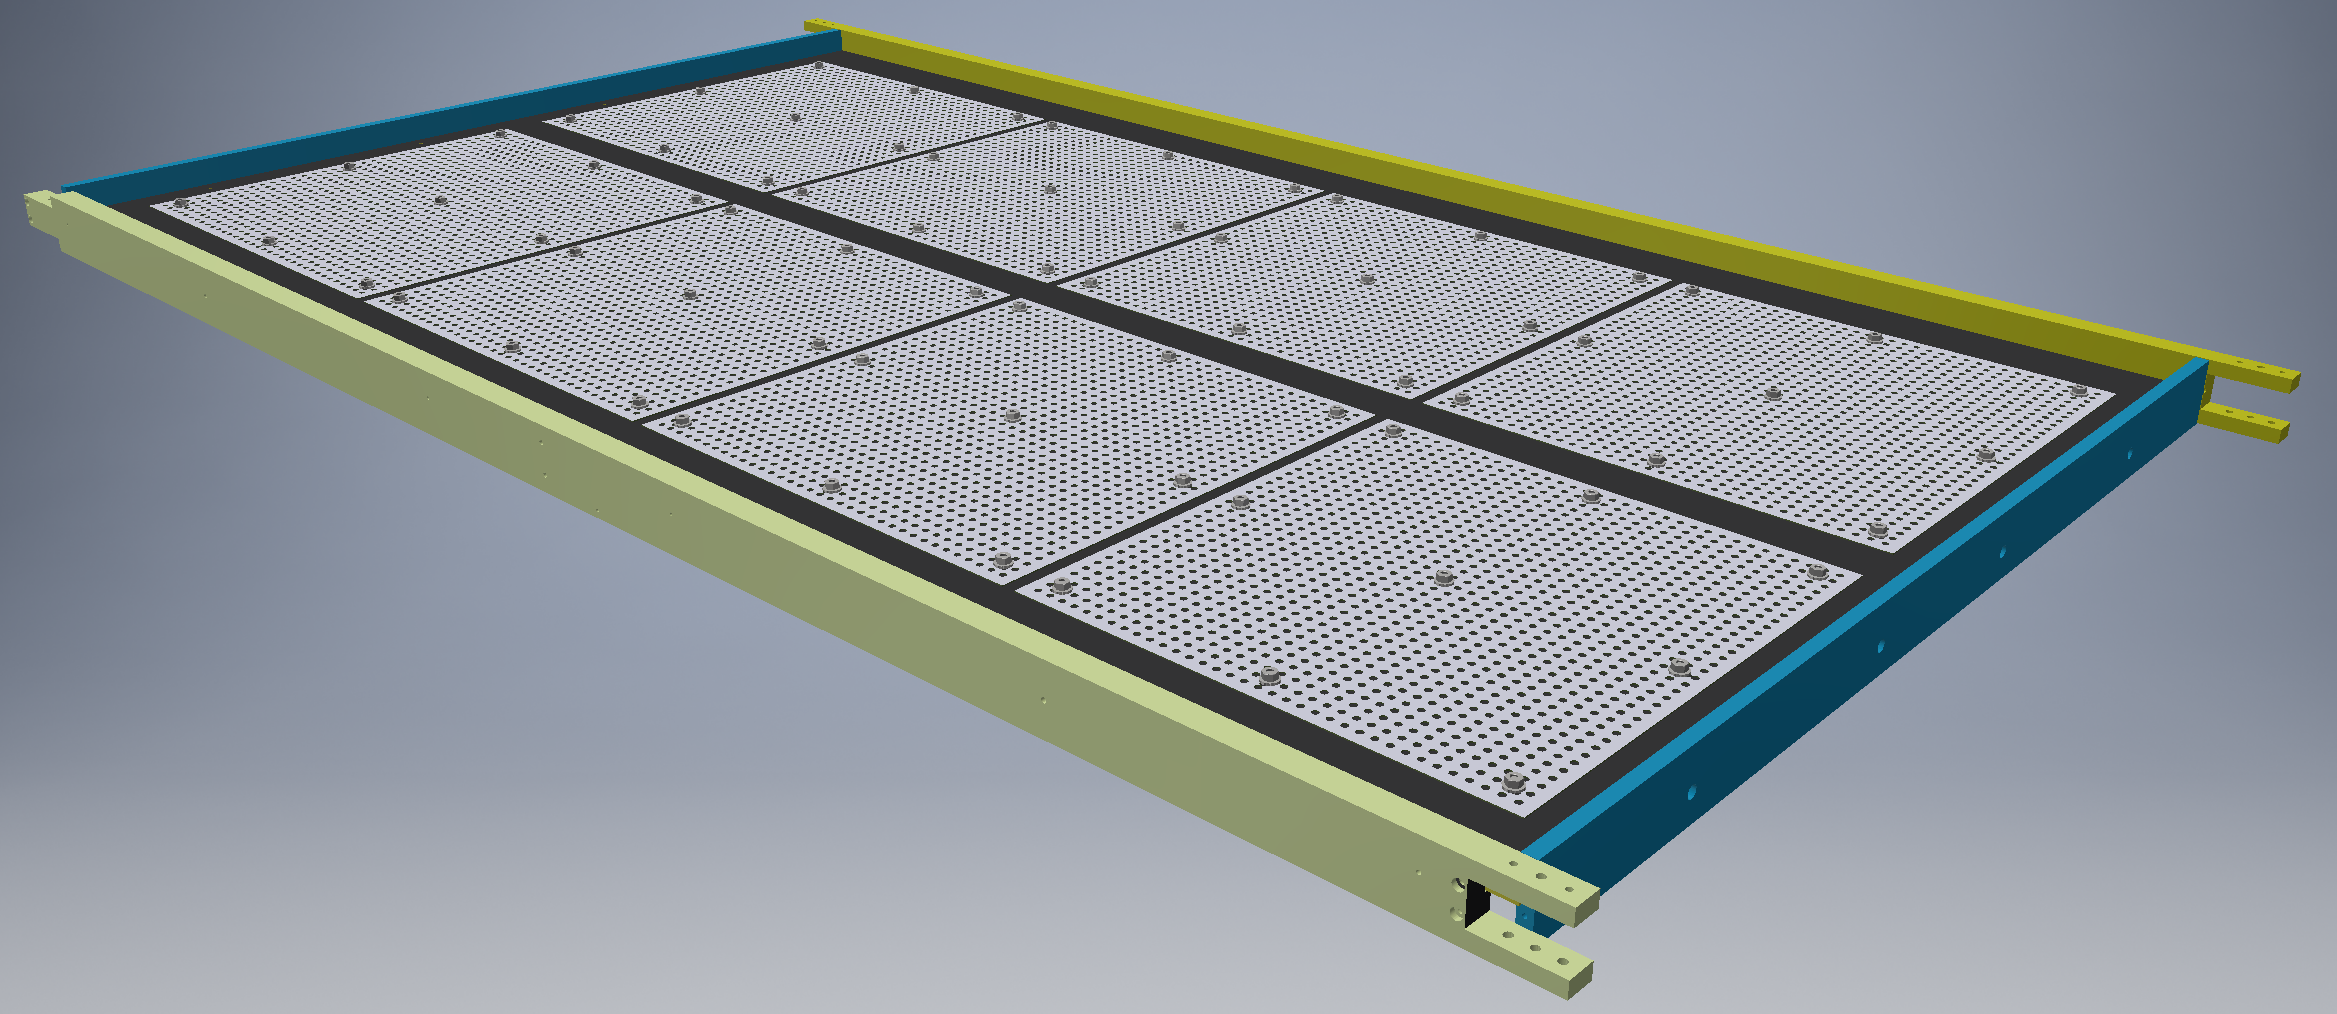
\includegraphics[width=0.9\textwidth]{ReflectorOnCPA.png}
\end{dunefigure}

\subsection{Calibration Laser Penetrations}

The calibration consortium is developing requirements for calibrating the \dword{tpc} \efield.  One existing technique is to use UV laser beams to ionize the \dword{lar} and generating straight tracks along known trajectories.  Since the \dword{fc} surrounds the \dword{tpc} active volume, one needs to either shoot through the gaps between the \dword{fc} profiles (as in \microboone), or make openings in the \dword{fc}  for the laser heads to pass through (as in SBND).    Figure~\ref{fig:SBND_laser}  shows the design of a corner of the SBND \dword{tpc} with a \dword{fc}  opening, and a calibration laser head through the opening.  Implementing such openings is straightforward if the openings are at the \dword{fc}  module boundaries.  Doing so through the interior surface of a \dword{fc} panel is more complicated, but still simpler than the beam plug we designed for \dword{pdsp}.  There will be some minor drift field distortion around the openings.  Preliminary \dwords{fea} have shown the field distortion to be negligible. 

\begin{dunefigure}[SBND laser arrangement]{fig:SBND_laser}{SBND field cage opening to allow a calibration laser head to pass through. (Credit: BNL)}
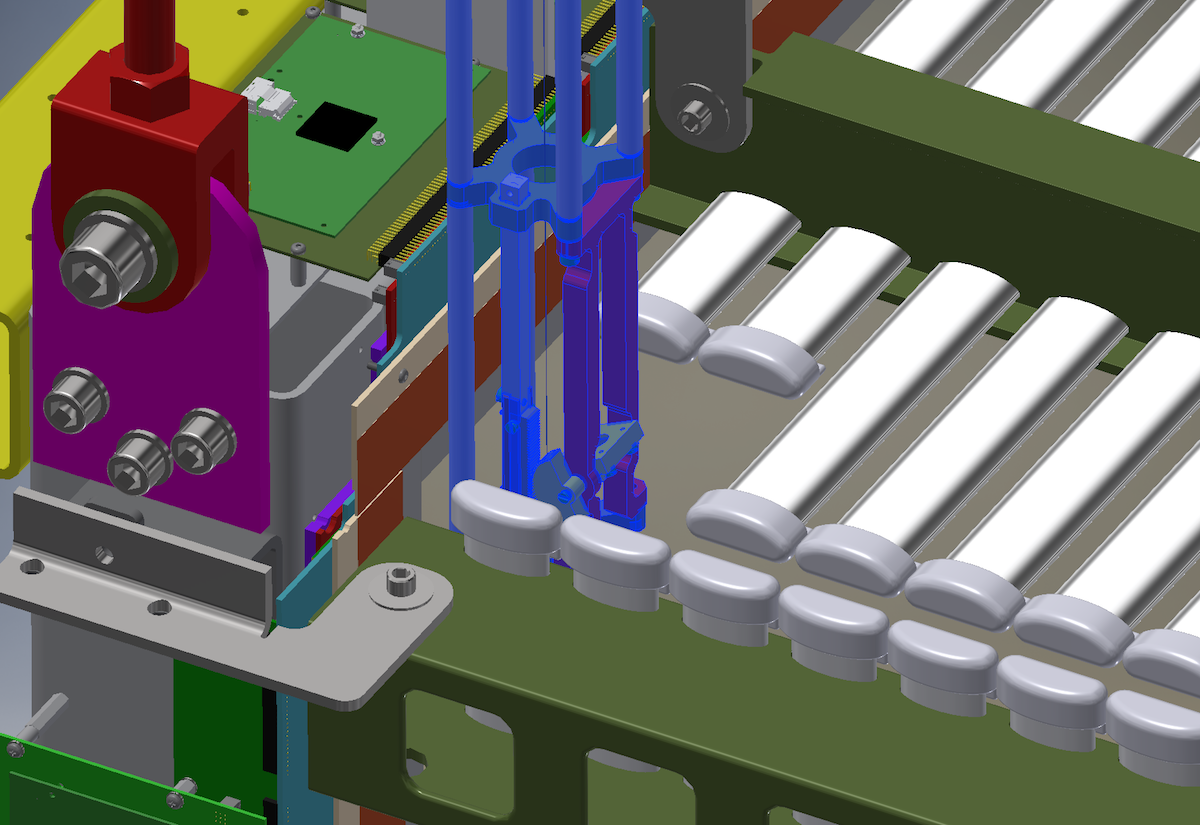
\includegraphics[width=0.7\textwidth]{SBND_Laser_Arrangement.png}
\end{dunefigure}


